
\documentclass[master]{thesis-uestc}
\usepackage{amssymb}

\title{时域积分方程时间步进算法及其快速算法}{The Time Marching Scheme of Time Domain
    Integral Equation and Corresponding Fast Algorithm}

\author{王稳}{Wang Wen}
\advisor{赖生建\chinesespace 副教授}{Dr. Shengjian Lai}
\school{物理电子学院}{School of Physical Electronics}
\major{无线电物理}{Radio Physics}
\studentnumber{201421040223}

% require all the usepackages here
% \usepackage{algorithm2e}

\begin{document}

% \makecover

% This is a template of mutiple files.
% The folders chapters/ and misc/ have the related files

% abstract
	
\begin{chineseabstract}
为了适应日益增长的宽带信号和非线性系统的工程应用,用于分析瞬态电磁散射问题的时域积分方程方法研究日趋活跃。本文以时域积分方程时间步进算法及其快速算法为研究课题,重点研究了时间步进算法的数值实现技术、后时稳定性问题以及两层平面波算法加速计算等,主要研究内容分为四部分。

……

\chinesekeyword{时域电磁散射,时域积分方程,时间步进算法,后时不稳定性,时域平面波算法}
\end{chineseabstract}



\begin{englishabstract}
	In real life, a large number of short text data are constantly generated, such as news text, comments on some aspects published by users on Meituan , Dianping and other websites.
	 The generation of text data is inevitably accompanied by the classification. 
	How to improve the classification efficiency and reduce the labor cost is the research direction of text classification.
	In addition, mining users' emotions from these massive data helps to accurately depict users, thus assisting the platform to provide targeted services. 
	However, most of the current methods ignore the relationship between words or between aspect words and context, which leads to poor classification performance. 

	This paper mainly studies the text classification algorithm based on graph model, including whole-text classification and aspect-level sentiment analysis task. 
	In order to improve the performance of the model, graph model combined with attention mechanism is used to mine the relationship between words, aspect words and text context. The main points of this thesis are summarized as follows:

	\begin{itemize}
		\item [1)] 
		An algorithm for whole text classification is proposed. This method constructs a graph for each text with words as nodes and the relationship between words as edges. 
		At the same time a hyper-node connected to all word nodes is established to represent the overall information of the text. 
		Then a graph convolutional neural network with an attention mechanism is used to learn the vector representations of hyper-node and word nodes, and finally the information of the two vectors is merged to improve the accuracy of text classification.
		\item [2)] 
		An aspect-level sentiment analysis algorithm is proposed. First, this method converts the text into a graph, and then constructs a hyper-node that connects all the words in the aspect words. 
		Learning word vector representation and hyper-node vector representation through graph convolutional neural network with attention mechanism and gating mechanism. 
		Finally, the hyper-node vector is used as the aspect words vector to realize the classification task with the text word vectors. 
		In addition, the BERT pre-training model is combined to further improve the classification performance
	\end{itemize}

	In general, the methods proposed in this article are based on graph model, using graph models to mine the relationship between text words and learn better word vector representations. 
	In addition, the attention mechanism and gating mechanism are used to control the transfer process of node information in the graph model. 
	Under the verification of a large number of data sets, the method proposed in this paper shows good performance and can be used for short text data.

	\englishkeyword{text classification, graph model, vector representation, aspect words, attention mechanism}
\end{englishabstract}




% table of contents
\thesistableofcontents

% thesis contents
\thesischapterexordium

\section{研究工作的背景与意义}
文本分类是自然语言处理较为关键的一项任务,比如邮件分类、观点挖掘、情感分析等\citing{sculley2007relaxed,saif2016contextual}。主要是通过对已知的一些文本进行训练学习,建立一个模型,挖掘文本中的深层次含义以及潜在规律,从而实现对未知文本的预测。例如,对于情感分类模型来说,通过输入用户的一句话或者一段话,实现对这段文本的分析,预测用户的情感,是消极还是积极。
随着互联网的飞速发展,网络中存在着大量的文本数据,尤其是类似于美团、豆瓣等数字平台上充满了用户行为留下来的大量文本,如富有感情色彩的评论,对电影的点评、对美食的评价。以及各大新闻论坛也包含了多种多样的新闻主题,例如政治类、财经类、娱乐类。从这些海量数据中挖掘出用户的情感,有助于精准地刻画用户,从而辅助平台进行针对性的提供服务。同时,用户对某一事项的不同方面进行评价,有利于对这些方面的不足之处进行改进以提升用户感知。过去文本分类涉及了许多人工操作,例如新闻主题分类,依赖于工作人员的主观判断,将对应的新闻主体分类至对应的主题类目下。随着文本的不断累积,加上每天大量的新增文本,为手工分类带来了巨大挑战,极大的增加了人力成本。自动化的文本分类出现,能够显著降低劳动成本,提升工作效率。
方面级的情感分类是指针对一段文本中指向的一个具体方面进行评价。例如一句话“这家餐馆的菜品很好吃,但是服务不太好”。这句话中主要提到了两个方面,一个是“菜品”,一个是“服务”。
并且针对这两个方面有着不同的评价,分别是“很好吃”和“不太好”。方面级情感分类模型实现的就是对于“菜品”这个方面进行打分评价。
相比于一般的文本分类针对的是一段文本或一句话进行的分类,方面级情感分类更加细分,需要捕捉到关键词的情感,更加注重于对某个关键词所表达的含义。
互联网的高速发展,各大平台将会产生大量的文本信息,自动化的分类文本,通过用户发布的文本内容,精准地刻画用户情感,从而支持业务决策,正是本论文研究的意义和价值所在。
传统的机器学习方法需要大量的手工提取特征的方式,增加了研究者的负担。而一些采用深度学习的方式在文本处理领域略有不足,例如很多算法忽略了文本的整体信息以及文本在语料库中的统计信息。尤其是在对于方面级目标词与文本内容之间关系的捕捉,很多模型仍有改进空间,因此文本分类任务的效率和准确度还有待提高。       
本学位论文研究基于图模型的文本分类算法,通过图模型有利于挖掘单词之间的关系信息,通过传递单词之间的信息,不断更新优化单词的向量表示,不断深入挖掘单词之间隐藏的语义信息,同时文本的具体含义与整个语料库的组成也有一定联系,通过图模型捕捉所有文本单词之间的关联有助于提升分类效果。方面级目标词与文本整体的单词之间也应该有较大关联,用户对方面目标所体现的情感应该仅有文本中的部分词有关,而大部分词应该是无关的,本论文希望通过图模型挖掘出这些内在关系,有助于进一步提升文本分类质量。

\section{国内外研究现状}
本论文旨在研究基于图模型的短文本分类算法研究,因此接下来主要介绍图网络模型算法和文本分类算法目前的研究现状。

\subsection{图网络模型算法研究}
在许多领域的数据都很容易转化成图结构。比如蛋白质组学、图像分析、社交网络和自然语言处理等。例如社交网络,每个用户都可以视作一个节点,他们之间的关系就可以构成一条条边,很自然的构成了一个图结构。由于图结构中的节点以及边都可以带有自己的属性信息,同时每个节点以及自己的邻居节点又可以构成一个新的拓扑图结构,因此基于图结构进行分析可以获取得到更加丰富的信息。
图是由节点和边组成的一种结构,节点可以是任意实体对象,比如一个用户,一个地点或是一个单词,而边可以表示为节点之间的特殊联系,比如用户之间的点赞,互相关注等。
\begin{figure}[htb]%\small tbp
	%	\vspace{-0.15cm}
	%	\setlength{\abovecaptionskip}{0pt}
	\setlength{\belowcaptionskip}{0pt}
	\centering
	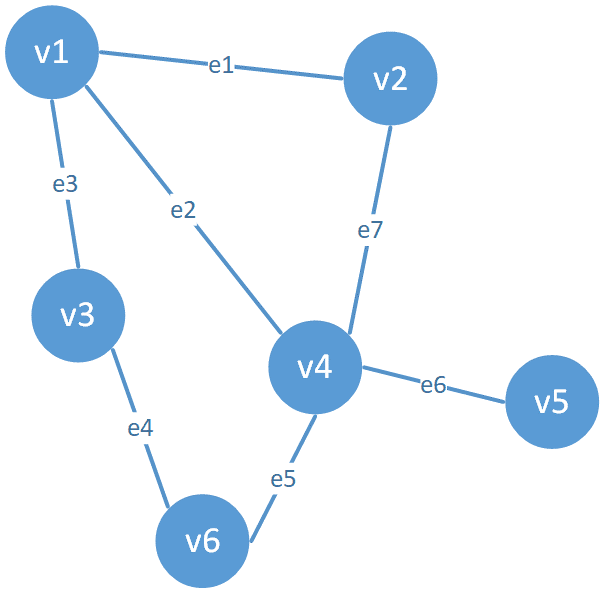
\includegraphics[width=0.4\textwidth]{pic/1-1.png}
	\caption{图结构}
	\label{graphStruc}
\end{figure}
如图\ref{graphStruc}所示是一个基本的图结构。节点之间以边连接,形成一个互相联系的结构。

近些年来,图神经网络已经被广泛应用于学习图的结构化向量表示。已经吸引了越来越多的学者\citing{xu2018powerful,cai2018comprehensive,wu2020comprehensive,zhou2018graph}。图神经网络主要是通过迭代的方式聚集信息,例如某个节点,通过从周围的邻居节点中汇聚信息,然后对信息进行处理,获得自身新的信息表示。再通过多次迭代,不断地更新自身的信息,获得丰富的特征向量表示。

图神经网络也包含多种,不同的网络也常对应不同的应用场景。许多传统的算法往往将图结构的数据压缩为链式结构,或者转换为树状结构,然后再使用链式神经网络(如RNN)或递归神经网络去处理。此时,图中的拓扑结构信息往往会有一定的损失,模型的性能也会受到压。基于此,Li\citing{li2015gated}提出了GGNN(Gated Graph Neural Networks)模型,该模型直接可以使用图结构信息,利用一个GRU模型实现信息的传递。不同节点之间应该具有不同的关系,节点之间的信息传递应该依赖于关系的强弱进行传导,即关系度较高的两个节点之间传递的信息应该占比更多,而关系度低的节点之间应该仅传递较少的信息。而传统的图神经网络往往忽略了这种节点之间信息传递的强弱,Petar Velickovic等人\citing{velivckovic2017graph}提出了一个基于注意力机制的图神经网络GAT(Graph Attention Networks)。该网络利用每个节点的嵌入表示,采用一个自主力机制学到节点之间的权重关系,再通过这种关系进行信息的传递。该网络相比于许多传统的图神经网络模型取得了非常好的效果,但其弊端就是增加了计算量,每次都需要计算相关的权重信息。

图神经网络中,用得较为广泛的就是Kipf\citing{kipf2016semi}等人提出的图卷积神经网络GCN(Graph Convolutional Networks)。GCN是一个多层的神经网络,首先我们定义一个图$G=\left(V,E\right)$,其中$V$代表图上的节点集合,$E$表示为节点之间的边的集合。GCN的包含输入一个节点的向量表示$X$,以及表示图节点关系的邻接矩阵$A$。在每一层神经网络中,每个节点只能从其直接邻居节点处汇聚信息,再加上自身的信息,形成新的表示。随着层次的加深,每个节点可以获取到更远的节点的信息,即获得了多跳的邻居信息。最终模型的输出就是每个节点的新的向量表示。GCN的传播计算如下
\begin{equation}\label{gcnFormula1}
    H^{\left(l+1\right)}=\sigma{{(\hat{D}}^{-\frac{1}{2}}\hat{A}\hat{D}}^{-\frac{1}{2}}H^{\left(l\right)}W^{\left(l\right)})
\end{equation}
\begin{equation}\label{gcnFormula2}
\hat{A}=A+I
\end{equation}
    其中$I$表示为单位矩阵,在原始的邻接矩阵上加上单位矩阵就是为了确保节点每次传递都能考虑到自身的信息。$H^{\left(l\right)}$表示为第l层的节点向量表示,$W^{\left(l\right)}$表示为第l层的参数。$\hat{D}$为$\hat{A}$的度矩阵。

\subsection{文本分类算法研究}
先前大量的文本分类工作主要通过对文本单词特征的提取分析,采用特征工程、机器学习或是深度学习等方式实现文本的分类。本文主要探讨的是两类文本分类,一种是定义为整体文本分类,即直接对于整个文本内容进行分类,例如一段文本。判断它是属于金融类或是娱乐类;一种是方面级情感分类,即是对文本中关注的某一个方面词进行分析,例如一段文本“这个店的服务很好,但是菜品不怎么样”,当方面词为‘服务’时,则分类结果是正面,当方面词为‘菜品’时,分类结果则是负面。两者采用的算法大致都是通用的,只是在部分细节上略有不同,方面级情感分类需要着重关注方面词的情感,在算法的研究上需要进一步精心设计

\subsubsection{整体文本分类算法研究现状}
(1)基于特征工程的算法和单词嵌入

在机器学习中,识别关键的以及找到相关的特征对于分类任务来说至关重要,文本分类任务也是如此。特征工程就是针对对应的文本挖掘其特征表示,最大限度地从原始数据中提取特征以供算法和模型使用。单词嵌入就是将文本中的单词用能代表其内在含义的一个向量进行表征,生成计算机能够识别的方式,进而实现分类任务。

K. Sparck Jones\citing{jones1972statistical}提出了IDF的方法,这个方法可通过与词频连用以减少语料库中隐性常用词的影响,TF便是词频。TF-IDF联合使用,可以作为输入特征进行分类。T. Mikolov等人\citing{mikolov2013efficient,mikolov2013distributed}提出了Word2Vec的方法,用以改进单词的向量表示。它采用了一个两层神经网络的基础架构,采用CBOW或是Skip-gram的模型训练文本单词,挖掘单词语义,将单词嵌入到一个高维的向量表示空间,最终获得每一个单词的一个向量表示。Glove\citing{pennington2014glove}方法也是一种学习单词表示的方法。他与word2vec类似,采用一个大型的语料库进行训练,将单词嵌入到高维空间,实现用一组向量表示单词。Glove方法相比于word2vec,考虑了这种全局词汇的共现信息,并且结合局部上下文窗口的方法的优点。Fastext\citing{joulin2016bag}可以用来学习词向量,也可以用来做一种快速简单有效的文本分类算法。但它也有一个缺点。因为它是对文本中的所有单词向量求和取平均,所以忽略了单词在文本中出现的顺序,可能导致错误的分类结果。

(2) 基于深度学习的算法

深度学习的概念源于人工神经网络的研究,例如含多个隐藏层的多层感知器就是一种深度学习结构。深度学习通过组合低层特征形成更加抽象的高层表示属性类别或特征,以发现数据的分布式特征表示。在自然语言处理方面,已提出了许多模型,尤其是文本分类这一任务上,更是不断有新的方法涌现。

RNN(Recurrent Neural Network)是一类用于处理序列数据的神经网络,广泛应用于各类序列上,备受各类研究者所关注\citing{salehinejad2017recent}。为解决RNN模型的梯度消失问题,提出了LSTM\citing{hochreiter1997long}(Long Short-Term Memory)长短期记忆网络。此外,还有一个RNN变种,GRU\citing{cho2014learning}(Gate Recurrent Unit)模型,它简化了LSTM的门机制,仅有一个重置门和更新门。Bi-LSTM\citing{schuster1997bidirectional}(Bidirectional Recurrent Neural Networks)即双向LSTM网络,考虑了文本的前后两个方向的信息。由Kim等人\citing{kim2014convolutional}提出了Text-CNN模型,将CNN(Convolutional Neural Networks)网络带入了文本处理领域。相继有人提出了RCNN\citing{lai2015recurrent},DRNN\citing{wang2018disconnected},TBCNN\citing{mou2014tbcnn}等基于CNN理论的模型用于文本分类。Liang Yao\citing{yao2019graph}等人提出了基于图卷积神经网络(GCN)的文本分类算法。该模型创新的将图卷积网络应用于文本分类领域,将图神经网络引向了新的方向。近年来最引人瞩目的用于自然语言处理的模型当属于transformer\citing{vaswani2017attention}以及bert\citing{devlin2018bert}模型,将自然语言处理推向了一个新的高度。

\subsubsection{方面级情感分类算法研究现状}
(1)基于传统机器学习的算法

Jiang等人\citing{jiang2011target}在面对应用在推特上的情感分类算法时,首先合并一些独立的特征,其次将一些相关的推文考虑进去作为新的特征,通过这些方式,改进分类算法。Wang等人\citing{wagner2014dcu}采用n-gram特征输入SVM中实现方面级的情感分类。Brychcín等人\citing{brychcin2014uwb}结合利用了约束性方法获取的特征以及非约束性方法获取的特征,将两种方式获得的特征结合通过最大熵分类器实现了方面级情感分类。

(2)基于深度学习的算法

Tang等人\citing{tang2015effective}提出采用LSTM模型捕获目标词与句子之间的关系用以实现方面级情感分类。Xue等人\citing{xue2018aspect}提出了一个采用了门机制的CNN模型,实验结果相比传统的LSTM模型具有更高的准确率以及计算速度。Huang等人\citing{huang2019parameterized}基于CNN模型提出PF-CNN和PG-CNN两种变种用以实现方面级情感分类。Han等人\citing{han2019multi}基于LSTM模型,融合了注意力机制关注方面级目标词以及上下文内容。Li等人\citing{li2019co}利用GRU模型学习文本序列信息,获取每个单词的隐藏层状态表示,此外还利用一个协同注意力机制学习目标是及上下文的向量表示,最后采用一个自注意力机制更新目标词与单词向量之间的权重,获得最终的用以文本分类的向量表示。Huang等人\citing{huang2018aspect}提出了一个AOA(Attention-over-Attention)模型,该模型可以捕捉到方面目标词与文本内容之间的关系信息。Zhang\citing{zhang2019aspect}提出采用图卷积神经网络(GCN)用以学习方面目标单词与文本内容单词之间的关系。首先它将文本通过解析树构建单词之间的关系,利用这种关系构建了一个有向图。该模型采用一个Bi-LSTM模型用以学习文本单词之间的隐藏状态表示,然后将每个单词的隐藏向量表示作为图卷积神经网络模型单词节点的初始化表示,通过几次卷积操作,生成新的向量表示。之后,找到对应的方面目标词在GCN模型的输出向量,再与Bi-LSTM模型的单词隐藏状态向量用注意力机制求得对应的关系权重。最后通过加权求和确定最终的情感向量表示。该方法实现了对句子语法的解析,以及语法对文本情感带来的影响,较为准确地区分了单词之间联系,找到了情感相关词汇,实验结果上相比一些方法有了一定提升。HaoTang\citing{tang2020dependency}结合bert、transformer以及GCN模型,进一步提升了模型的准确率。

\section{主要研究内容}
本文针对基于图模型的文本分类算法进行研究。根据文本内容,将单词作为节点,单词之间的邻接关系或是依赖关系作为边,构成图结构,再采用图模型算法进行文本分析,实现文本分类任务。基于此算法,再引入方面词处理,进一步实现方面级情感分类。
因此,本文主要实现两个方面的研究,一是针对整体文本分类算法进行研究设计,采用图模型算法提升分类任务准确率。二是实现方面级情感分类。基于第一点的研究基础,将方面词考虑进模型,对算法进行改进,实现处理方面级情感分类任务,并以此提高分类准确率。
\subsection{整体文本分类算法设计}
传统的文本分类算法忽略文本在语料库中整体的统计信息,以及单词之间的互相影响。因为单词之间互有关联,尤其是同一个句子中的单词含义应该与整个句子的语义有关,而通常的单词嵌入模型每个词向量仅有一种。本文第三章中将文本中的每个单词视作一个节点,采用滑动窗口构建拓扑图结构,采用图模型将单词之间的信息通过图网络互相传递,重新学得更符合整个句子语义的单词的表示。同时还结合每个单词在整个语料库的统计信息,进一步生成代表整个文本含义的特征向量表示。对于单词向量再采用常规的CNN模型、LSTM模型进行分析,再与单词统计信息学的到特征向量相结合,最终实现文本分类任务。
\subsection{方面级情感分析算法设计}
方面级的目标词与文本内容单词之前应该存在许多联系,如果能够挖掘它们之间的内在关系,便能进一步学到情感信息。本文第四章利用第一点的算法进行扩充,将方面词引入通过图网络模型对单词之间的联系进行挖掘,重新学得文本中每个单词的向量以及方面目标词的向量。同时采用门控机制,进行遗忘和选择记忆不同层节点信息。新学得的词向量更符合文本含义,并且词向量之间也构建了诸多内在联系。接着采用attention机制找出目标词和文本单词之间的关系,即找到最能表达目标词情感的其他单词,最后通过组合这些单词,获得特征向量,实现方面级情感分类任务,提升分类效果。
\section{论文组织结构}
本文共分为五章,每章的主要内容如下:
第一章 绪论。本章主要从根据现实情况分析了文本分类任务的研究背景以及意义,同时简单介绍了图模型相关理论以及文本分类算法以及方面级情感分析算法的国内外研究现状。并对本文的主要研究内容进行了概括。

第二章 相关理论及技术。本章首先介绍了文本的处理方式,以及常用的例如word2vec、glove等单词向量表示学习方法。随后总结了图模型相关理论,着重介绍了GCN网络原理及对关键问题进行了详细描述。接着介绍文本分类任务中常用的门控机制、CNN模型以及注意力机制原理。最后介绍了目前较为流行的Bert模型。

第三章 基于图模型的整体文本分类算法。本章首先介绍了整体文本分类问题的定义,然后对算法的核心思想进行了简单的阐述,接着对算法原理以及算法框架的各个组成部分进行了详细的介绍,
包括图文本的构建方式和超节点的建立方法。随后对实验使用的数据集以及对比方法、评价指标进行了简单介绍,最后通过实验结果证明该模型的有效性。

第四章 基于基于图模型的方面级情感分析算法。本章首先介绍了方面级情感分析任务的描述和定义。接着对本章提出的算法原理进行了详细的阐述。然后介绍了实验数据、对比实验以及验证方法。
最后在多个数据集上进行实验,对比各个方法之间的优劣,通过实验数据表明本章提出的方法在方面级情感分析任务上取得不错的效果。

第五章 总结与展望。总结全文的工作内容,展望未来的研究方向。 

\chapter{相关理论及技术}
本章首先对文本分类任务进行简单介绍以及单词嵌入表示如word2vec,glove等学习方式。本章主要围绕了基于图模型文本分类模型的相关理论以及关键技术。包括图模型,图卷积神经网络(GCN),注意力机制,以及本文将会使用的技术和深度学习模型如TF-IDF、GRU、CNN、Bert等。
\section{文本分类任务}
在如今人类活动中产生了大量的文本数据,如美团、大众点评上对美食的各类评论,豆瓣上对书籍、电影的评价,以及人类历史活动中各类简短信息,例如微博、推特,新闻摘要等。这类都是一些短文本,对这类短文本进行分析一方面有助于实现快速归类,对于不同类型的文本内容进行整理;
另一方面针对用户的平均分析用户行为,改善服务。文本分类涉及多种情况,本文主要探讨整体文本分类算法以及方面级情感分析算法。
\subsection{整体文本分类和方面级情感分析}
(1)整体文本分类

对于整体文本分类来说,目的是对整段文本的描述进行判断,以数据集R8为例,该数据集为分类任务常用的文本数据集,为路透社新闻文本,共有八个分类。

\begin{figure}[htb]%\small tbp
	\setlength{\belowcaptionskip}{0pt}
	\centering
	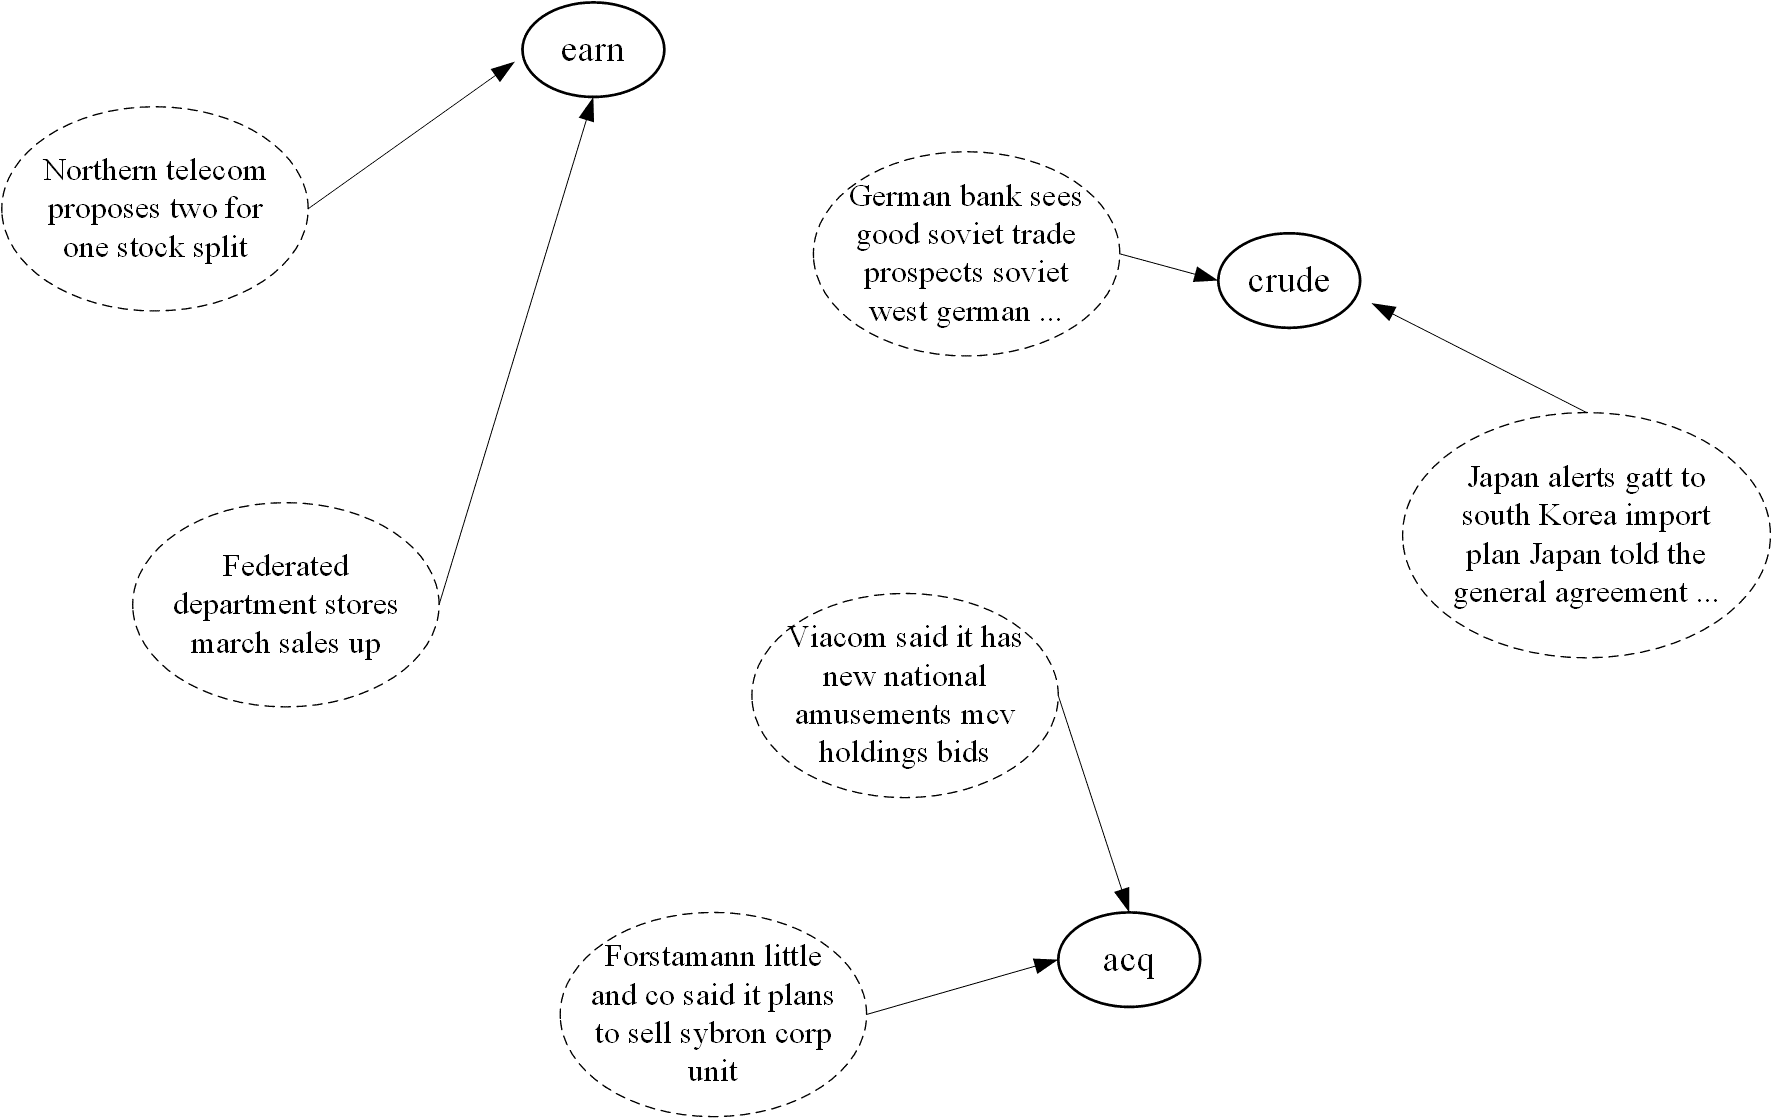
\includegraphics[width=0.8\textwidth]{pic/2-1.png}
	\caption{R8数据集}
	\label{R8datasets}
\end{figure}
如图\ref{R8datasets}所示,截取了数据集中三个分类标签,分别是earn、acq和crude。每个类别下都有对应的文本,代表了这个文本的分类属于这个标签。
从图\ref{R8datasets}可以看出来,整体文本分类任务是对整句话进行分类,一般一个文本只属于一个类别。比如“Federated department stores march sales up”这句话,
从文意可以看出描述了联邦百货公司3月销售额上升,正好符合earn标签的含义,因此对于这段文本可以分类为earn。
总的来说,本文定义的整体文本分类任务是针对于一个文本整体进行分类,判断该段文本从属的标签类别,一般情况下一个文本只有一个标签。

(2)方面级情感分析任务

方面级情感分析任务不同于整体文本分类任务,它是对文本中存在的方面目标词进行分类,而不是整段文本,因此,一段文本,对于方面级情感分析任务来说,存在多个方面目标词,那么就可能存在多个类别标签。方面目标词即可以是一个单词也可以是一个词组。本文以semeval14数据集为例,该数据集是14年推特的文本数据集,常用来做情感分析。
\begin{figure}[htb]%\small tbp
	\setlength{\belowcaptionskip}{0pt}
	\centering
	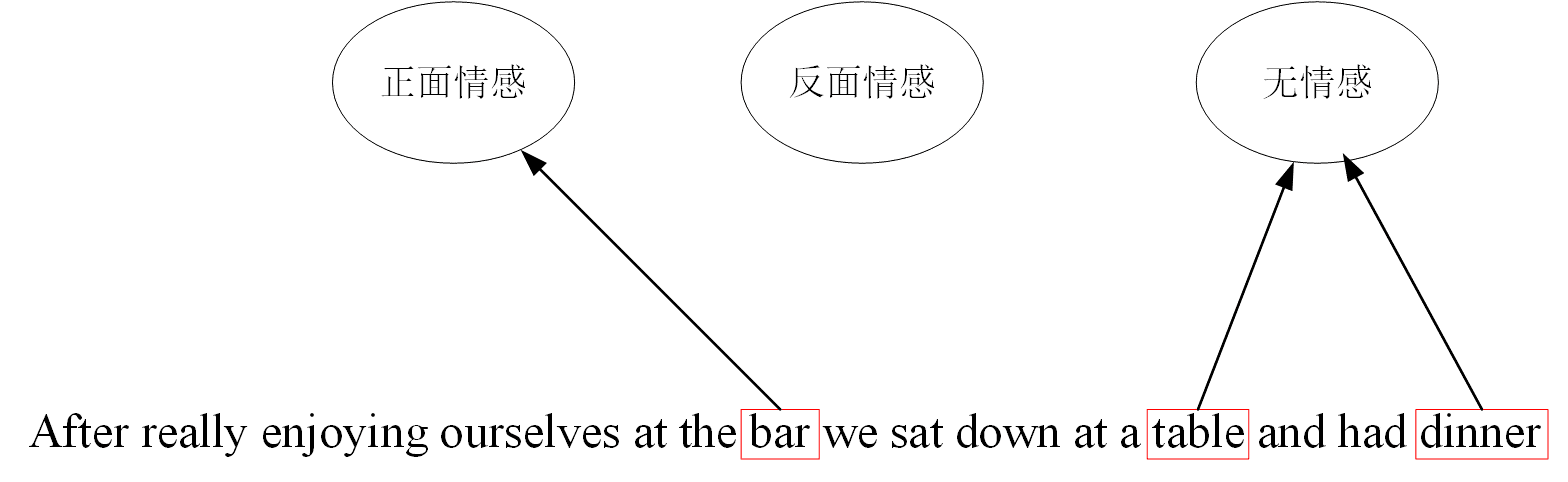
\includegraphics[width=0.8\textwidth]{pic/2-2.png}
	\caption{semeval14数据集}
	\label{semeval14datasets}
\end{figure}

从图\ref{semeval14datasets}可以看出,该段文本共有三个由红色方框标注出来的方面目标词,分别是‘bar’、‘table’、‘dinner’。
方面级情感分析任务就是需要实现分别对这三个词的情感进行分析,而不是对整个文本进行分类。因此相比于整体文本分类任务来说,需要更精细的设计。比如‘bar’这个词,从文本描述来看,最能体现这个词语情感信息的词应该是‘enjoying’,而‘enjoying’代表了正面的情感,因此对于‘bar’这个方面目标词把它归于‘正面情感’这个标签;对于‘table’和‘dinner’,这句话没有明显的情感,仅仅作为描述语句或是补充,因此没有特别的情感色彩,把它们归属于‘无情感’的标签下。所以,对于方面级情感分析任务来说,需要根据方面目标词进行分析,把握该词汇与其他具有情感色彩的词汇之间的关系,分析具体的情感色彩指代。
同一个句子中可能存在多个情感色彩词,并且词的含义可能是相反的,一个可能代表了积极正面的情感,另一个可能是消极的负面情感。相比于整体文本分类任务来说,更具有难度。
\section{单词嵌入表示}
文本数据不同于一般的图像、音频等数据。图像数据本身就具有意义,是天然带有的属性,即使没有经过训练的生物或许也能分辨不同的图片。而文本数据是人类的高层的抽象的思维信息表达的工具,具有高度抽象特征。在图像处理中,一张图片通常可以用一个矩阵表示,其中每个坐标的点即为像素点的值,矩阵中每个数值都具有一定意义,且矩阵属于稠密矩阵。而一段文本通常有多个单词构成,每个单词可以由一个向量表示,如图\ref{textEmb}所示。
\begin{figure}[htb]%\small tbp
	\setlength{\belowcaptionskip}{0pt}
	\centering
	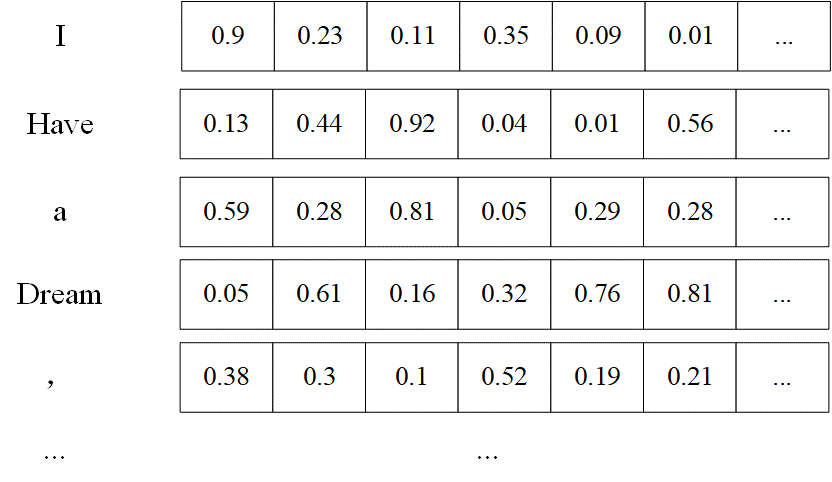
\includegraphics[width=0.8\textwidth]{pic/2-3.png}
	\caption{文本向量表示}
	\label{textEmb}
\end{figure}

如图\ref{textEmb}所示,一句话由多个向量组成,每个单词有一个向量表示,不同于图片矩阵,向量中的每个单一的值没有具体的含义,所有的值构成一个向量才具有表示为单词信息的含义。向量中的值一般取决于表示的方法。如采用one-hot的表示方式,向量中仅含有一个为1的值,其他值为0。向量的维度由单词个数决定,如一个单词量为2000的词库,构成的单词向量即为1*2000的向量。如单词Dream位于该词库中第二个位置,它的向量表示可能是(0,1,0,0,…,0),另一个单词Have可能位于第1000个位置,那么它的向量表示可能就是(0,0,…,1,…,0,0)。每个单词都由一个唯一的向量表示。虽然这种方式非常简单,但同时带来许多问题。1.向量维度随着单词数量而增加,当面对几万甚至几十万的词库时显得力不从心。2.每个单词向量都仅仅由0,1构成,没有具体含义,难以把握单词之间的联系。

Hinton提出的Distributed Representation\citing{hinton1986learning}思想可以用以学习词向量解决这个问题。这类词向量的表示一般类似于(0.22,-0.17,…,0.65,0.01)这种。而现如今常用的学习词向量的方法有word2vec,glove等。

Word2vec它采用了一个两层神经网络的基础架构,采用CBOW或是Skip-gram的模型训练文本单词,挖掘单词语义,将单词嵌入到一个高维的向量表示空间,最终获得每一个单词的一个向量表示。
\begin{figure}[htb]%\small tbp
	\setlength{\belowcaptionskip}{0pt}
	\centering
	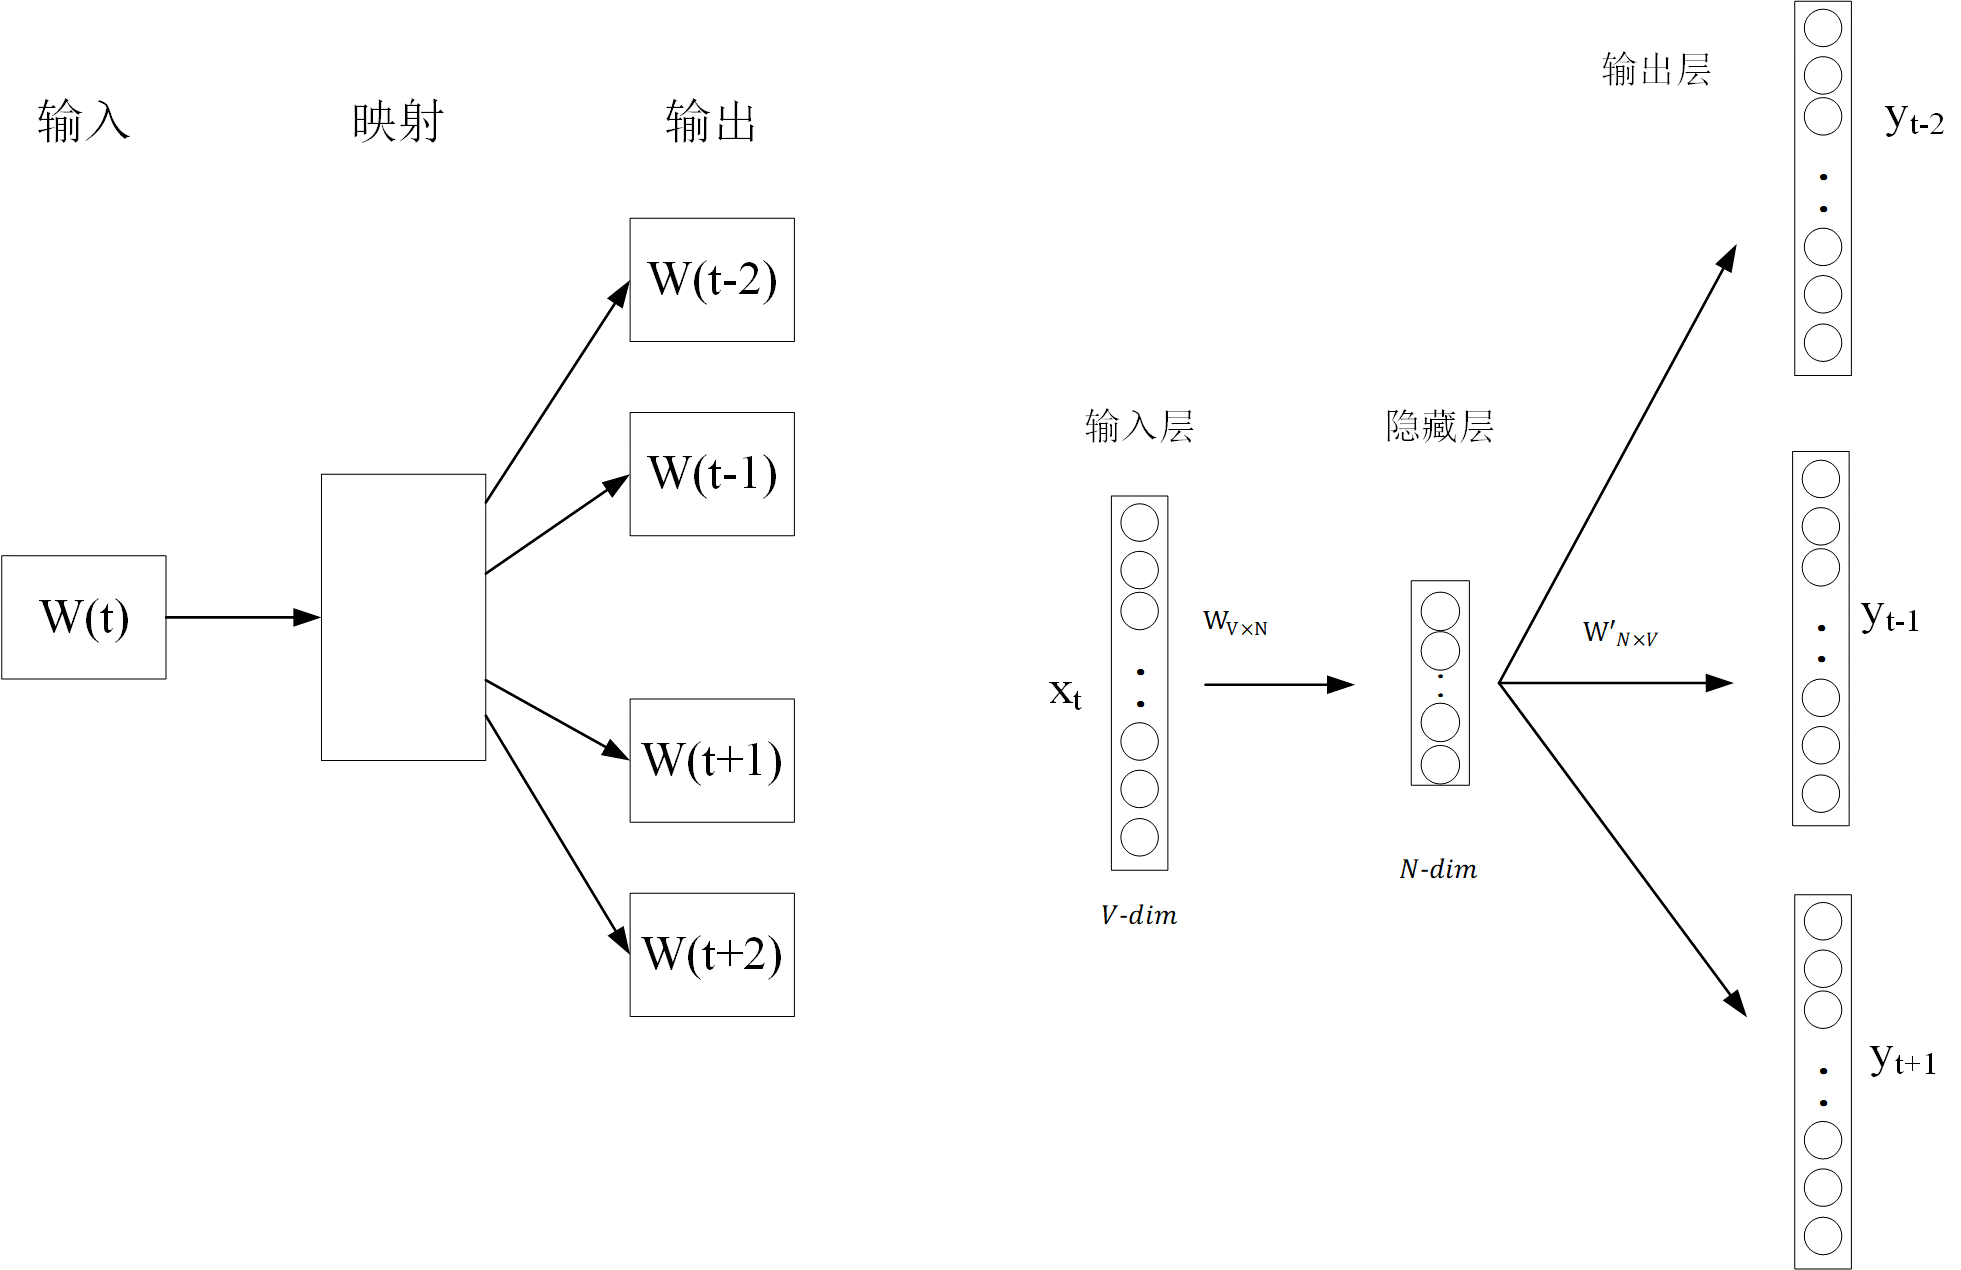
\includegraphics[width=0.8\textwidth]{pic/2-4.png}
	\caption{skip-gram模型}
	\label{skip-gram}
\end{figure}

Skip-gram模型如图\ref{skip-gram}所示,图左为模型架构,即通过中间单词预测该单词的上下文词。神经网络模型如图右所示。Skip-gram训练模型仅包含一个没有激活函数的隐藏层,和使用softmax激活函数的输出层。对于一个包含V个单词的数据集,模型的输入是一个V维的one-hot向量,经过一个$W_{V\times N}$的矩阵转化为N维的向量$h_t$,通常N远远小于V,这样一来可以将单词维度下降到很小,而所谓的$W_{V\times N}$参数矩阵即是我们需要学习的词嵌入矩阵。之后在经过一个${W^\prime}_{N\times V}$的参数矩阵,将隐藏向量$h_t$转为一个V维的向量,经过softmax激活函数,向量中的每个值都在0-1之间,代表着预测的单词的概率。计算公式如下:
\begin{equation}\label{skip-gramFormula1}
	h_t=Wx_t
\end{equation}
\begin{equation}\label{skip-gramFormula2}
	u_{t-1}=W^{\prime}h_t
\end{equation}
\begin{equation}\label{skip-gramFormula3}
	p\left(w_{t-1}\middle|w_t\right)=y_{t-1}=\frac{exp\left(u_{t-1}\right)}{\sum_{j=1}^{V}exp\left(u_j\right)}
\end{equation}
其中$W$,$W^\prime$分别为$V\times N$维,$N\times V$维的参数矩阵,$p\left(w_{t-1}\middle|\ w_t\right)$表示单词$w_t$的上下文预测单词$w_{t-1}$的概率。
\begin{figure}[htb]%\small tbp
	\setlength{\belowcaptionskip}{0pt}
	\centering
	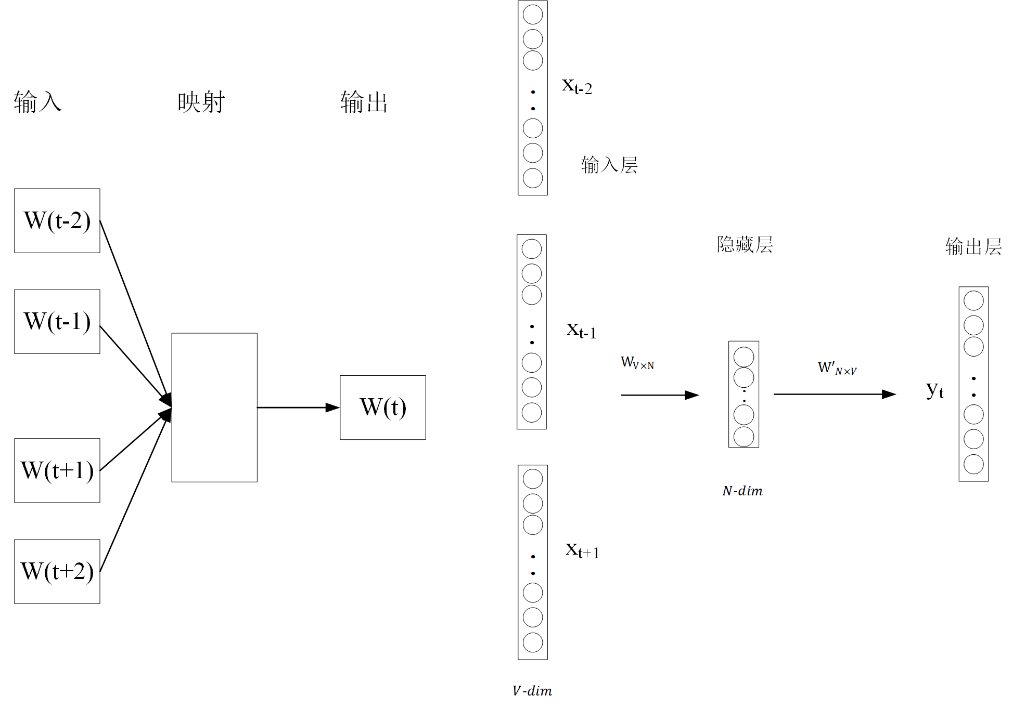
\includegraphics[width=0.8\textwidth]{pic/2-5.png}
	\caption{CBOW模型}
	\label{CBOW}
\end{figure}

CBOW模型如图\ref{CBOW}所示,图左为COBW模型架构,它与skip-gram相反,通过上下文信息预测中间词。首先是通过上下文多个单词计算隐层向量$h_t$,计算公式如\ref{CBOWFormula1},主要采用上下文C个单词的加权和得出。接着与skip-gram类似通过输出层转化为V维向量,再通过softmax预测。
\begin{equation}\label{CBOWFormula1}
	h_t=\frac{1}{C}W\sum_{i=1}^{c}x_i
\end{equation}

Glove方法也是一种学习单词表示的方法。他与word2vec类似,采用一个大型的语料库进行训练,将单词嵌入到高维空间,实现用一组向量表示单词。但是word2vec的CBOW和skip-gram方法是基于局部上下文窗口的,忽略了单词之间的共现信息。Glove方法的提出,考虑了这种全局词汇的共现信息,并且结合局部上下文窗口的方法的优点,来学习词向量,相比word2vec效果得到了一定的提升。
Glove目标函数可以近似为:
\begin{equation}\label{CBOWFormula1}
	F\left(w_i-w_j,w_k\right)=\frac{p_{ik}}{p_{jk}}
\end{equation}
其中$w_i$,$w_j$,$w_k$分别代表单词i,j,k的表示向量,$p_{ik}$代表单词k出现在单词i上下文的概率。Glove的目标就是找到函数F的表示空间,从而得到所有单词的向量表示。
\section{图模型相关理论}
现实生活中存在着大量的图结构数据,比如分子结构,社交网络,地理位置。这些数据的关键点在于都有一个可抽象化的节点,比如社交网络中的用户,以及连接这些节点的边即关系,比如社交网络中用户的关注、用户的点赞评论等交互。如何去利用这些图数据那就首先需要获取这些图数据中节点或是边的有效表示\citing{hamilton2017representation}。现如今已有大量关于图模型数据处理的研究\citing{scarselli2008graph,battaglia2016interaction,zhang2018end}。

图神经网络(GNN)主要是利用神经网络去学习节点表示$h_v$,或是整个图的向量表示$h_G$。通常每个节点v会有一个初始的向量表示$x_v$,经过图模型计算学习获得新的表示。而学习的过程主要是一种信息聚集的过程,即节点首先会从自己的邻居节点聚集信息,随着每一轮的聚集,当前节点将会获取到更远处节点的信息,即经过k轮迭代,当前节点或许可以得到k-跳的邻居节点信息,如下公式所示:
\begin{equation}\label{GNNFormula1}
	a_v^kf=\left(h_u^{k-1}:u\in\mathcal{N}\left(v\right)\right)
\end{equation}
\begin{equation}\label{GNNFormula2}
	h_v^k=g\left(\left[h_v^{k-1},a_v^k\right]\right)
\end{equation}

其中k表示第k次聚集,$a_v^k$表示节点v从其邻居节点集合$\mathcal{N}\left(v\right)$聚集得到的信息。聚集过程可以采用简单的加权和,也可以根据算法自定义方式。主要功能就是将邻居节点的信息融合得到一个新的向量,即得到一个具有丰富信息的向量。随后节点v再将上一次迭代获取的到的向量表示与当前聚集轮次获得到的邻居信息融合起来,组成新的该节点的向量表示。随着次数的增多,当前节点将会获取到多跳邻居节点的信息,使得当前节点的向量表示更加丰富,融入了多种信息,表达更加全面。

\subsection{图卷积神经网络}
Kipf提出的图卷积神经网络\ref{kipf2016semi}是一种直接在图上进行计算的半监督学习模型。首先定义一个图$G=(V,E)$,其中$V\left(\left|V\right|=n\right)$表示图中的节点,共有n个,E表示图中的边的集合。如图\ref{topoFig}所示每个节点都与其他某个或多个节点进行相连,构成了一个拓扑图。可以用邻接矩阵$A$表示节点之间的关系,如图\ref{adjA}所示。其中两个节点之间如果有边,则矩阵对应位置的值为1,反之则为0。此外邻接矩阵对应的度矩阵$D$如图\ref{digD}所示。其中$D_{ij}=\sum_{j}\ A_{ij}$。
\begin{figure}[htb]%\small tbp
	\setlength{\belowcaptionskip}{0pt}
	\centering
	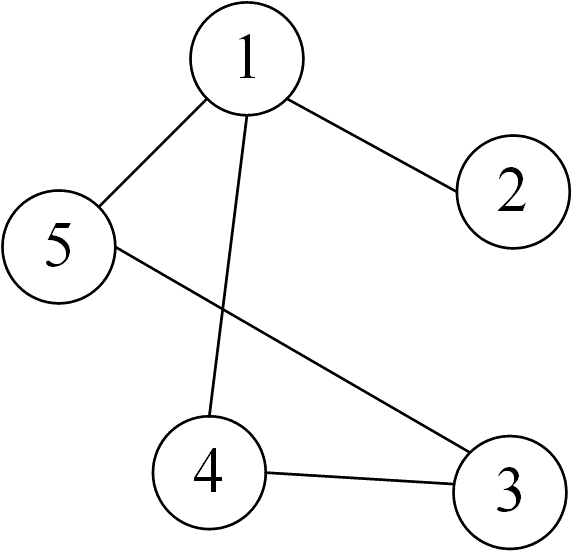
\includegraphics[width=0.4\textwidth]{pic/2-6.png}
	\caption{拓扑图}
	\label{topoFig}
\end{figure}
\begin{figure}[htb]%\small tbp
	\setlength{\belowcaptionskip}{0pt}
	\centering
	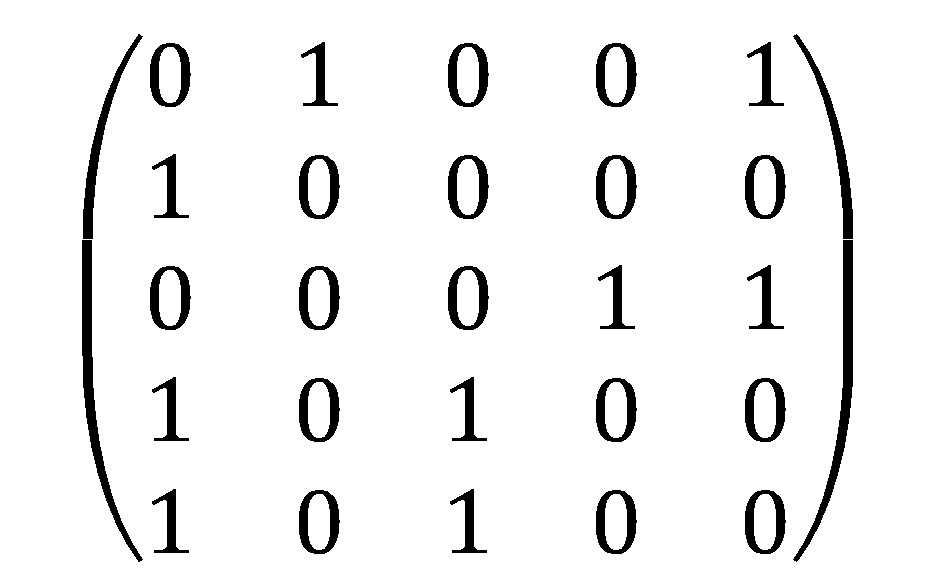
\includegraphics[width=0.4\textwidth]{pic/2-7.jpg}
	\caption{邻接矩阵A}
	\label{adjA}
\end{figure}
\begin{figure}[htb]%\small tbp
	\setlength{\belowcaptionskip}{0pt}
	\centering
	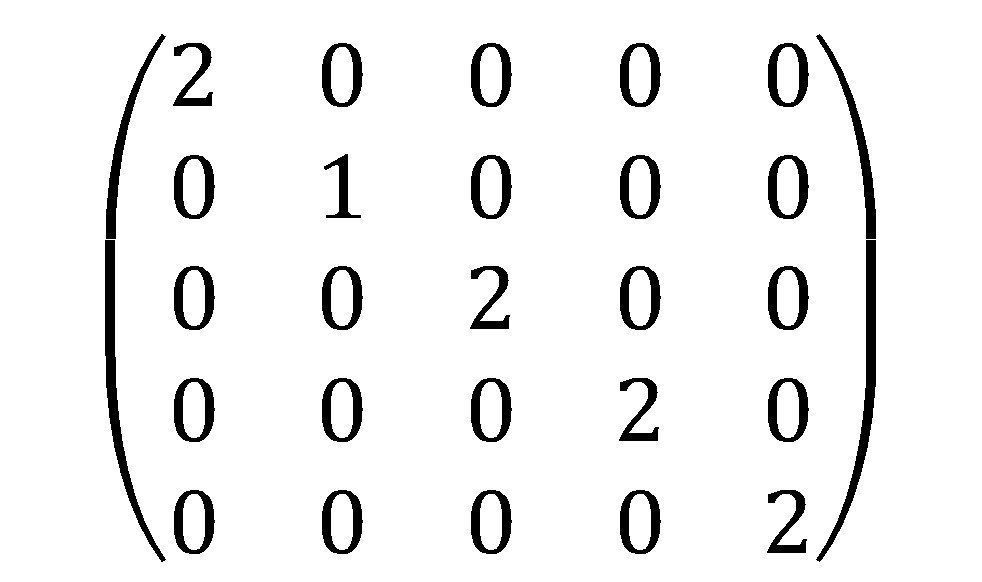
\includegraphics[width=0.4\textwidth]{pic/2-8.jpg}
	\caption{度矩阵D}
	\label{digD}
\end{figure}

假设每个节点$v_i$具有$m$维的特征向量$x_i\in R^m$,因此n节点构成特征向量矩阵$X\in R^{n\times m}$。节点信息在图中的传播主要沿着边进行,即通过边将每个节点的潜在信息进行传递。一个节点获取到来自其他节点的信息,将这些信息进行融合更新自身节点的信息,从而使得当前节点的信息更加丰富。每一次的信息传递都会增加额外的节点信息。刚开始,只会获取得到与当前节点直接相连的其他邻居节点的信息,同理邻居节点也会获取得到其邻居节点的信息,随着传递次数的增加,当前节点获取到的信息不仅仅是直接相邻的节点信息,更能获取得到更远的不相邻节点的信息。Kipf提出的图卷积计算方式可以由下公式得到:
\begin{equation}\label{GNNFormula1}
	H^{\left(l+1\right)}=\sigma{{(\hat{D}}^{-\frac{1}{2}}\hat{A}\hat{D}}^{-\frac{1}{2}}H^{\left(l\right)}W^{\left(l\right)})
\end{equation}

其中$\hat{A}=A+I$, $I$表示为单位矩阵。在原始的邻接矩阵上加上单位矩阵就是为了确保节点每次传递都能考虑到自身的信息。$H^{\left(l\right)}$表示为第$l$层的节点向量表示,$W^{\left(l\right)}$表示为第$l$层的参数。$\hat{D}$为$\hat{A}$的度矩阵。

\section{注意力机制}
\begin{figure}[htb]%\small tbp
	\setlength{\belowcaptionskip}{0pt}
	\centering
	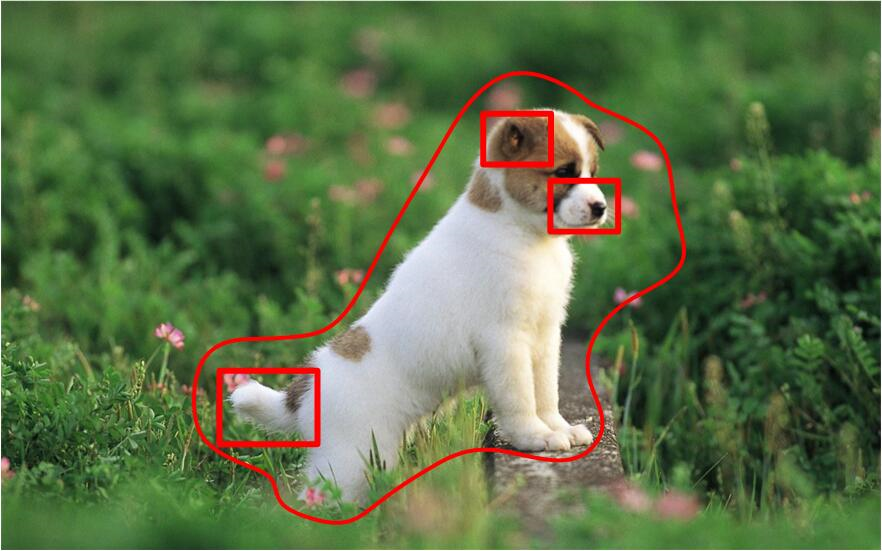
\includegraphics[width=0.6\textwidth]{pic/2-9.png}
	\caption{人类观察狗狗图}
	\label{watchDog}
\end{figure}
注意力机制就是模拟人类对视觉的处理,是源于对人类视觉的研究。人类通过眼睛观察周围场景,能够从有限的时间中快速挖掘场景中的信息,正是由于人类大脑提供的处理机制-注意力机制,让人能在复杂的场景中快速适应。人类对场景观察时,大部分情况下仅关注于重点区域,将大部分注意力资源都投入到这些区域中,而尽量忽略一些无关紧要的信息,实现资源的有限分配。这是人类与生俱来的赖以生存的机制,人类视觉的注意力机制大大提高了视觉信息处理的时效性以及准确性。如图\ref{watchDog}所示,人类对于图片的识别时,识别这张图像是猫还是狗,首先可能会把观察重点放在图片中存在的那个动物上,然后忽略图片中其他的场景,如图中红色线框所示,人类观察时,忽略了这个动物存在的场景,即忽略了周边的花草,因为这些信息对分析这个动物类别没有帮助。
确定了大致区域后,视觉进一步将注意力放在耳朵,嘴巴,尾巴等位置上,从这些有限的区域就能大致分析出这个动物属于狗,而不是猫。因此,注意力机制对于实现有限的资源调度以及提升准确率(因为避免了类似花草场景的干扰)具有很大帮助。

注意力机制之前主要大量用于视觉处理,首次用于自然语言处理领域可以追溯到Bahdanau\citing{bahdanau2014neural}等人在2014年提出的基于RNN的编码-解码翻译模型。该篇文章不同于以往的翻译模型—在编码阶段将所有单词编码为单一向量$c$,这样的处理方式会使得模型在压缩的信息的过程中不得不忽略一些信息,从而使得翻译模型在面对长句子时处理能力很差。Bahdanau并没有固定编码向量$c$,而是根据解码层每一步的隐藏状态与编码时每个单词的隐藏向量计算得到不断变化的编码向量$c_i$。这种技巧就是一种注意力机制的处理方式,大大提高了模型的性能。
\begin{figure}[htb]%\small tbp
	\setlength{\belowcaptionskip}{0pt}
	\centering
	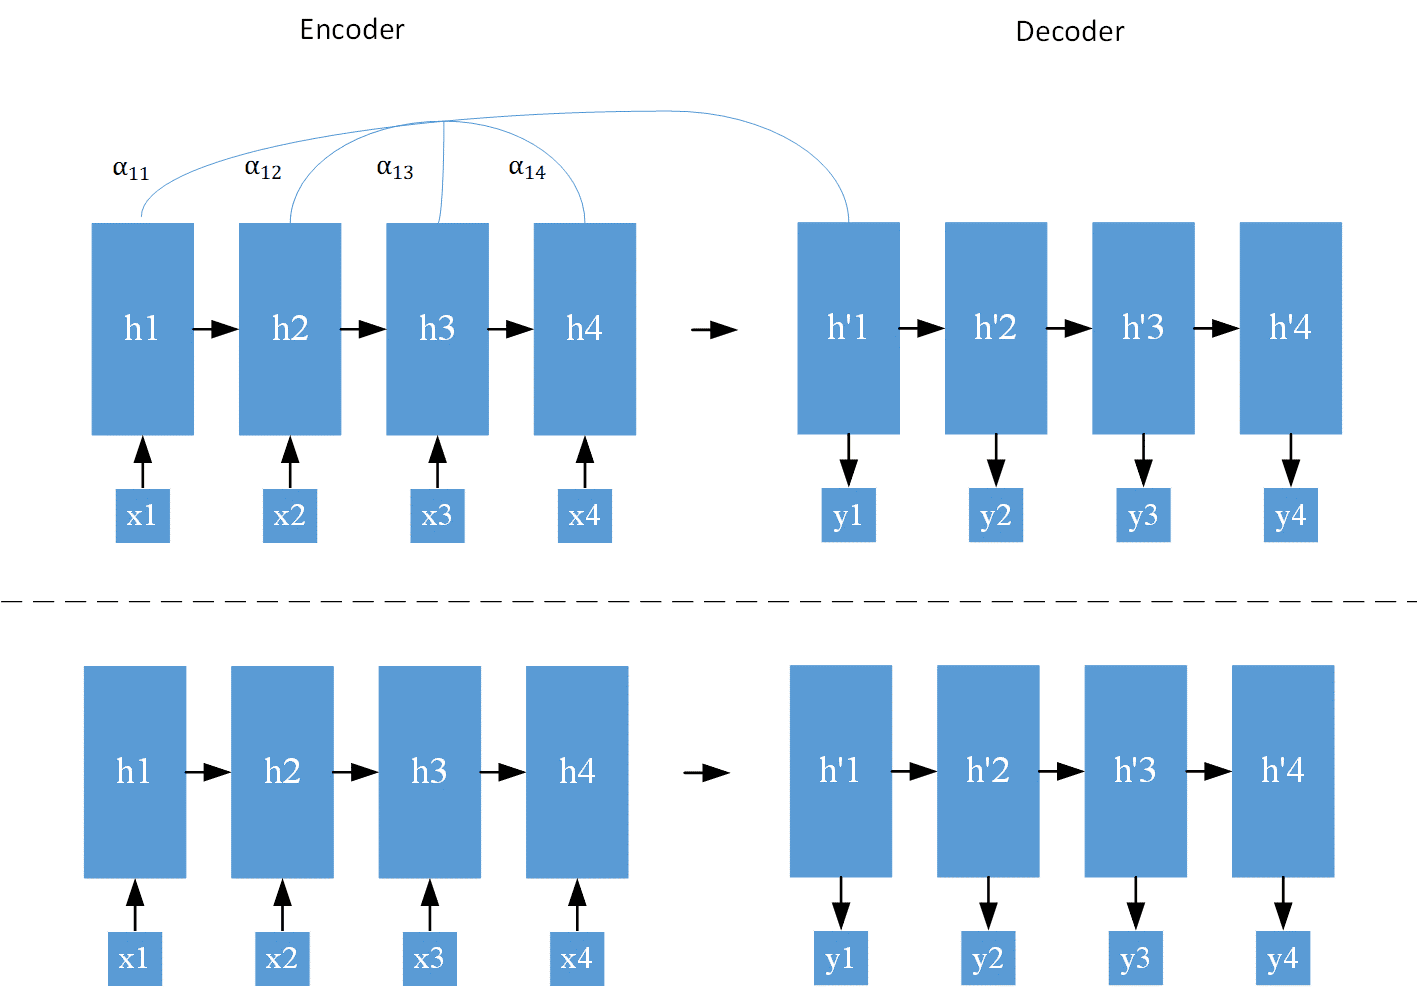
\includegraphics[width=0.8\textwidth]{pic/2-10.png}
	\caption{注意力机制RNN(上)与普通RNN(下)}
	\label{rnn-att}
\end{figure}

如图\ref{rnn-att}所示就是采用了注意力机制(图上)和普通RNN模型(图下)的差异。以下介绍几种常用的注意力机制使用方式。
\subsection{注意力机制计算}
在深度学习模型中,注意力机制计算可以简化为三类向量,一个是查询向量,即query向量,简称为$q$;一个是关键词向量,即key向量,简称为$k$;最后一类是值向量,即value向量,简称为$v$。通常查询向量$q$是一种特定于任务的向量,例如在上文提到的翻译模型中,$q$就是上一个隐藏状态向量。而$k$向量便是用来计算注意力分数的向量,如上文提到的翻译模型中的单词隐藏向量。$v$向量便是最终用于加权求和的向量。

注意力机制实现过程主要由以下公式计算得到\ref{attFormula1}、\ref{attFormula2}、\ref{attFormula3}。
\begin{equation}\label{attFormula1}
	a_i = score(q,k_i)
\end{equation}
\begin{equation}\label{attFormula2}
	\alpha_i = \frac{exp(a_i)}{\sum_{j}exp(a_j)}
\end{equation}
\begin{equation}\label{attFormula3}
	c=\sum_{j}v_j* \alpha_j
\end{equation}

其中$score(q,k_i)$为根据关键向量$k_i$与查询向量$q$计算得到的注意力分数,有不同的计算方式。
luong\citing{luong2015effective}提出公式\ref{scoreFormula1}和\ref{scoreFormula2}所示的计算方式,其中$W_a$是一个可训练的参数矩阵。
Vaswani\citing{vaswani2017attention}采用公式\ref{scoreFormula3}的计算方式,其中$n$是向量的维度。
\begin{equation}\label{scoreFormula1}
	score(q,k_i)=q^\mathrm{T}k_i
\end{equation}
\begin{equation}\label{scoreFormula2}
	score(q,k_i)=q^\mathrm{T}W_ak_i
\end{equation}
\begin{equation}\label{scoreFormula3}
	score(q,k_i)=\frac{q^\mathrm{T}k_i}{\sqrt{n}}
\end{equation}
\subsection{自注意力与多头注意力机制}

\begin{figure}[htb]%\small tbp
	\setlength{\belowcaptionskip}{0pt}
	\centering
	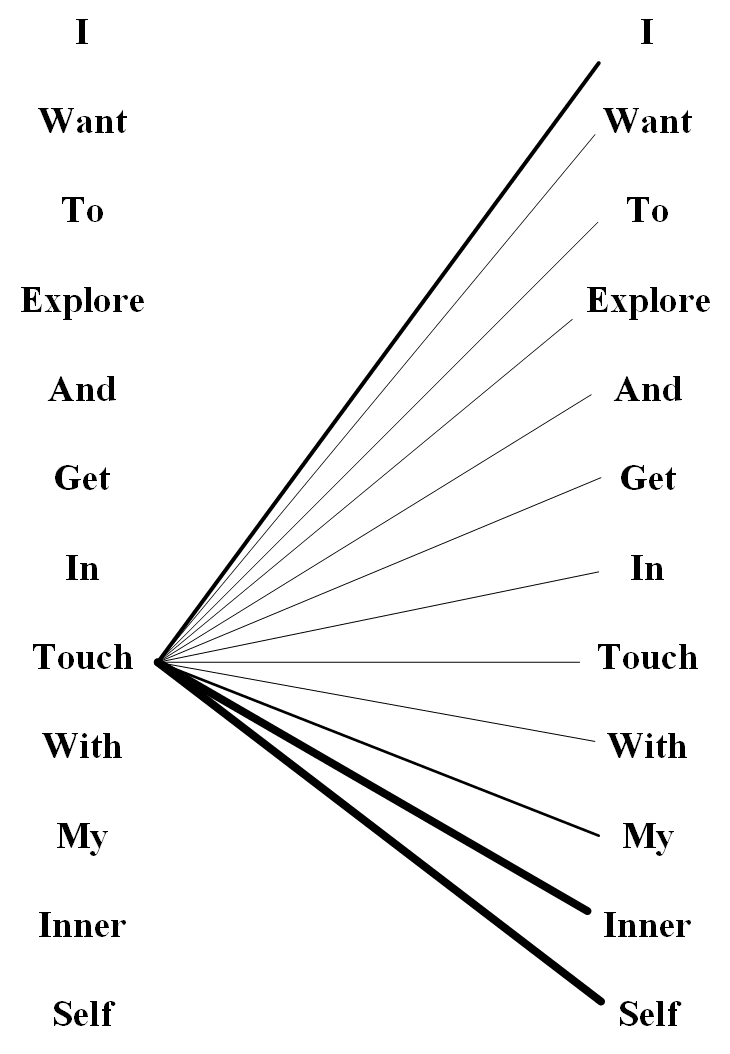
\includegraphics[width=0.4\textwidth]{pic/2-11.png}
	\caption{自注意力机制}
	\label{self-att}
\end{figure}
自注意力机制是一种关联单个序列的不同位置的注意力机制。通过计算每个位置与其他所有位置上的信息的注意力权重,从而获取得到对于当前位置最重要的一些信息,同时也能保留那些不重要的信息,更新当前位置的向量表示
。如图\ref{self-att}所示,单词‘touch’会计算所有其他单词的之间的注意力分数,分数大小由线段粗细为例,‘touch’可能更加关注于‘inner self’等单词,因此分配的权重也会更高,对于其他
单词分配的权重会低一些。Lin\citing{lin2017structured}采用注意力机制提出一个可解释性的文本嵌入模型,用于情感分析等任务上取得优异的结果。
\begin{figure}[htb]%\small tbp
	\setlength{\belowcaptionskip}{0pt}
	\centering
	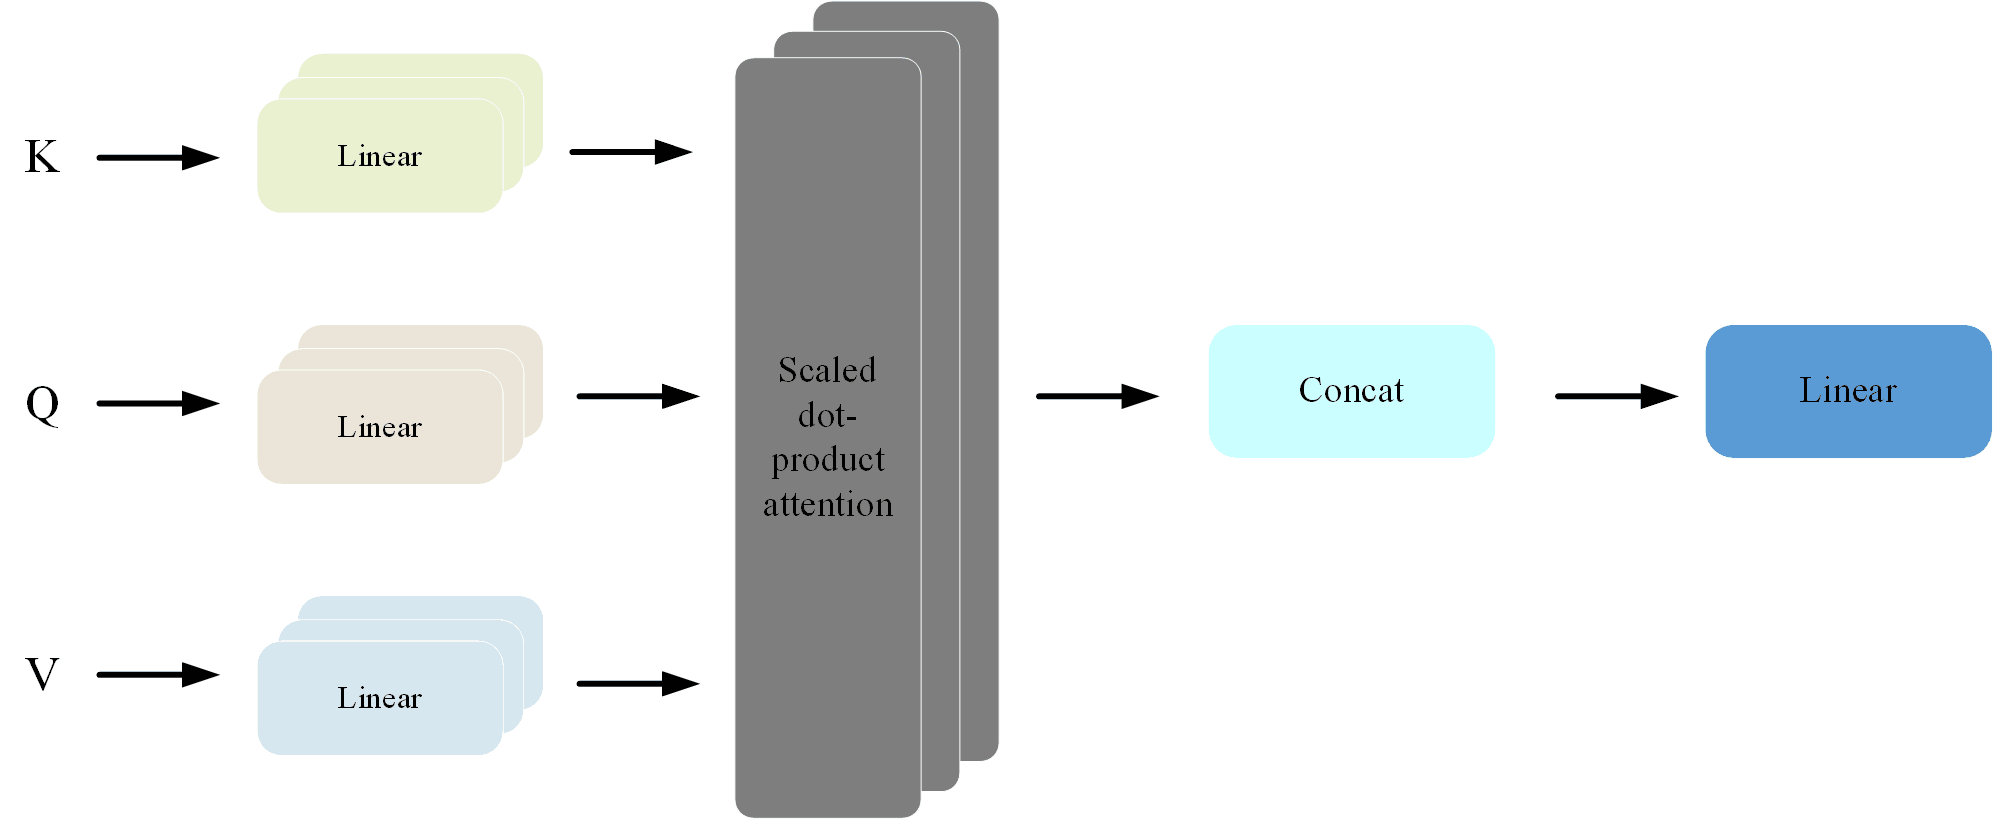
\includegraphics[width=0.8\textwidth]{pic/2-12.png}
	\caption{多头注意力机制}
	\label{muti-att}
\end{figure}

多头注意力机制首次由Vaswani\citing{vaswani2017attention}等人提出。首先将Query,Key,Value进行线性变换
,这里将计算多个线性变换,每个线性变换的参数均不一样。每一次的计算就是所谓的一个‘头’。然后采用放缩点积(scaled dot-Product attention)
方式计算,如公式\ref{scoreFormula3}所示。最后将结果拼接通过再通过一个线性变换层输出得到。如图\ref{muti-att}所示。
这样的好处就是可以允许模型在不同的表示子空间里学习到不同的相关信息。
\section{其他相关技术模型}
\subsection{TF-IDF}
TF-IDF是一种统计方法,用以评估一个字词对于一个文件集或一个语料库中的其中一份文件的重要程度。字词的重要性随着它在文件中出现的次数成正比增加,但同时会随着它在语料库中出现的频率成反比下降。
K. Sparck Jones\citing{jones1972statistical}提出了IDF的方法,这个方法可通过与词频连用以减少语料库中隐性常用词的影响。计算方法如公式\ref{idf}:
\begin{equation}\label{idf}
	idf=lg\frac{\left|D\right|}{\left|\{j:t_{i\ }\in d_j\}\right|}
\end{equation}

其中$D$表示语料库中的文件总数,分母包含单词$t_i$的文件数目。TF即是单词词频,表示如公式\ref{tf}所示:
\begin{equation}\label{tf}
	tf=\frac{n_i}{\sum n_k}
\end{equation}

其中$n_i$代表单词$i$出现的次数,分母为所有单词出现的总次数。TF-IDF联合使用,可以表示为:如果某个词或短语在一篇文章中出现的频率TF高,并且在其他文章中很少出现,则认为此词或者短语具有很好的类别区分能力。因此可以根据这个方法来做分类。

\subsection{CNN文本分类}
CNN(Convolutional Neural Networks)模型是一类包含卷积计算且具有深度结构的前馈神经网络(Feedforward Neural Networks),是深度学习(deep learning)的代表算法之一。卷积神经网络(CNN)具有表征学习能力,最主要的特征就是具有平移不变性。CNN最早可以追溯到日本科学家福岛邦彦\citing{fukushima1982neocognitron}提出的一个包含卷积层、池化层的神经网络结构。虽然中间消沉了一段时间,仅仅有一些少量性的研究工作,但Hinton等人提出的Alexnet\citing{krizhevsky2017imagenet},颠覆了图像识别领域,从而再次吸引了大量人员对于CNN的研究。
CNN主要应用于视频、图像等领域,由Kim等人\citing{kim2014convolutional}提出了Text-CNN模型,将CNN网络带入了文本处理领域。
\begin{figure}[htb]%\small tbp
	\setlength{\belowcaptionskip}{0pt}
	\centering
	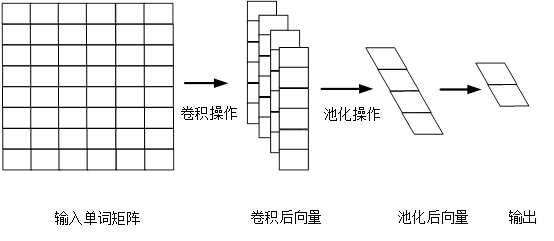
\includegraphics[width=0.8\textwidth]{pic/2-13.png}
	\caption{CNN模型}
	\label{cnn}
\end{figure}

如图\ref{cnn}所示,一段文本可以用一个$N\ast D$的矩阵表示,其中$N$代表文本中单词的数目,$D$代表单词向量的维度。经过一个$k\ast D$大小的卷积核操作,其中$k$表示为每次卷积操作的单词数,再经过一个池化层,得到一维向量表示。将多个卷积核操作获得的向量进行拼接,获得这段文本的向量表示。最后将这个向量表示输入一个分类器实现文本分类等任务。该CNN模型相比RNN模型,在一些比较的数据集来看,准确率相差不大,但是对于一些情感分类的文本来说有一定的优势。CNN最具优势的一点就是它能够并行计算,因而相比传统的RNN模型,计算速度有了较大提升,极大地缩短了训练时常,在一些比较注重实效的场景下,可以选择CNN模型。

\subsection{门控机制}
\begin{figure}[htb]%\small tbp
	\setlength{\belowcaptionskip}{0pt}
	\centering
	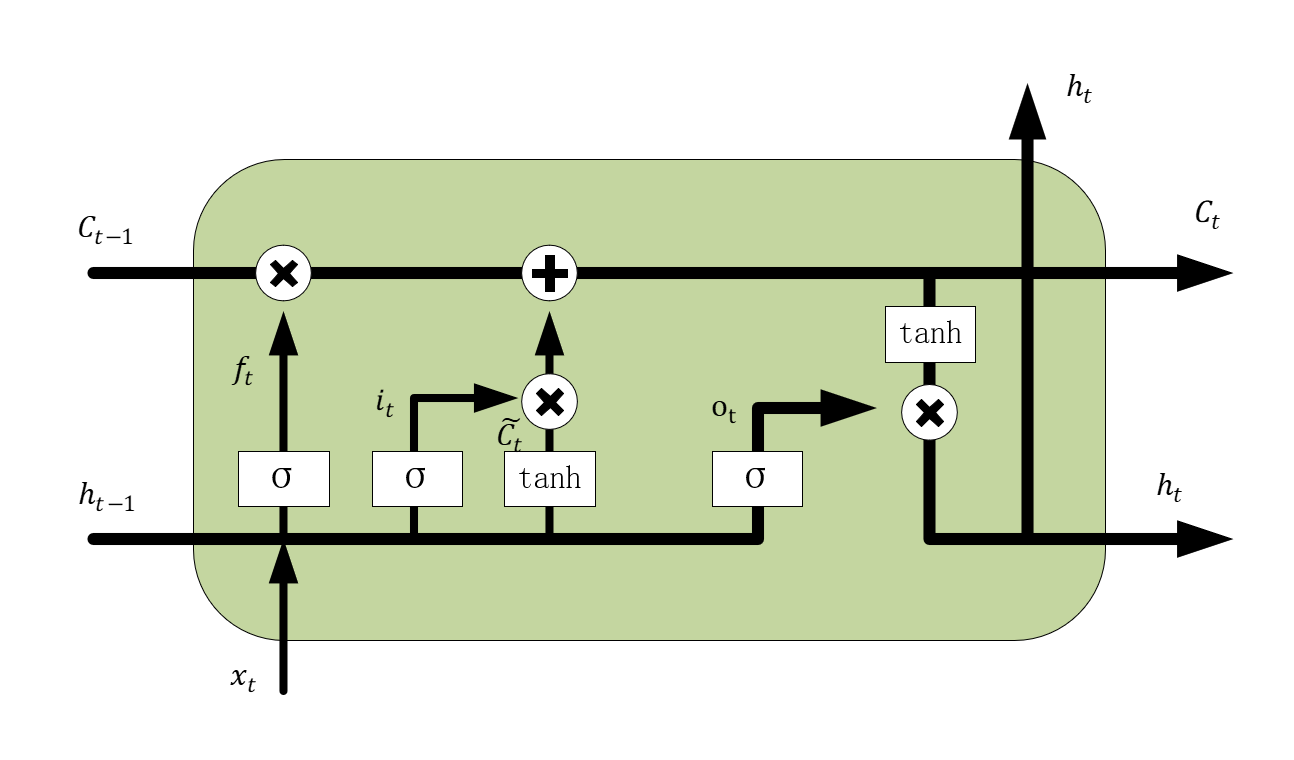
\includegraphics[width=0.8\textwidth]{pic/2-14.png}
	\caption{LSTM模型}
	\label{lstm}
\end{figure}
LSTM、GRU网络中采用了门控机制,实现了对短期记忆与长期记忆的结合,提升了模型性能,并且一定程度上解决了RNN模型的梯度消失问题。
如图\ref{lstm}所示,LSTM模型采用了门结构,门就是一个选择信息通过或抛弃的机制。计算过程如下:
\begin{equation}\label{LSTMFormula1}
	f_t=\sigma(W_f\bullet\left[h_{t-1},x_t\right]+b_f)
\end{equation}
\begin{equation}\label{LSTMFormula2}
	i_t=\sigma\left(W_i\bullet\left[h_{t-1},x_t\right]+b_i\right)
\end{equation}
\begin{equation}\label{LSTMFormula3}
	\widetilde{C_t}=tanh\left(W_c\bullet\left[h_{t-1},x_t\right]+b_c\right)
\end{equation}
\begin{equation}\label{LSTMFormula4}
	C_t=f_t\ast C_{t-1}+i_t\ast \widetilde{C_t}
\end{equation}
\begin{equation}\label{LSTMFormula5}
	o_t=\sigma\left(W_o\bullet\left[h_{t-1},x_t\right]+b_o\right)
\end{equation}
\begin{equation}\label{LSTMFormula6}
	h_t=o_t\ast tanh\left(C_t\right)
\end{equation}

LSTM中包含三个门结构,遗忘门、输入门以及输出门。遗忘门的计算首先通过之前的信息$h_{t-1}$以及当前输入信息$x_t$计算得到$f_t$,一个在0-1之前的数,用以选择哪些信息需要丢弃。随后再利用输入门计算$i_t$用以决定更新信息的量以及一个待选择的信息$\widetilde{C_t}$,最后计算出新的信息$C_t$。输出门利用$h_{t-1}$和$x_t$计算需要的特征,结合$C_t$信息,输出最终的向量表示$h_t$。该向量表示就可以代表整个文本的抽象特征,可以用来作文本分类任务。
\subsection{BERT模型}
BERT\citing{devlin2018bert}模型是基于transformer模型\citing{vaswani2017attention}提出的
\begin{figure}[htb]%\small tbp
	\setlength{\belowcaptionskip}{0pt}
	\centering
	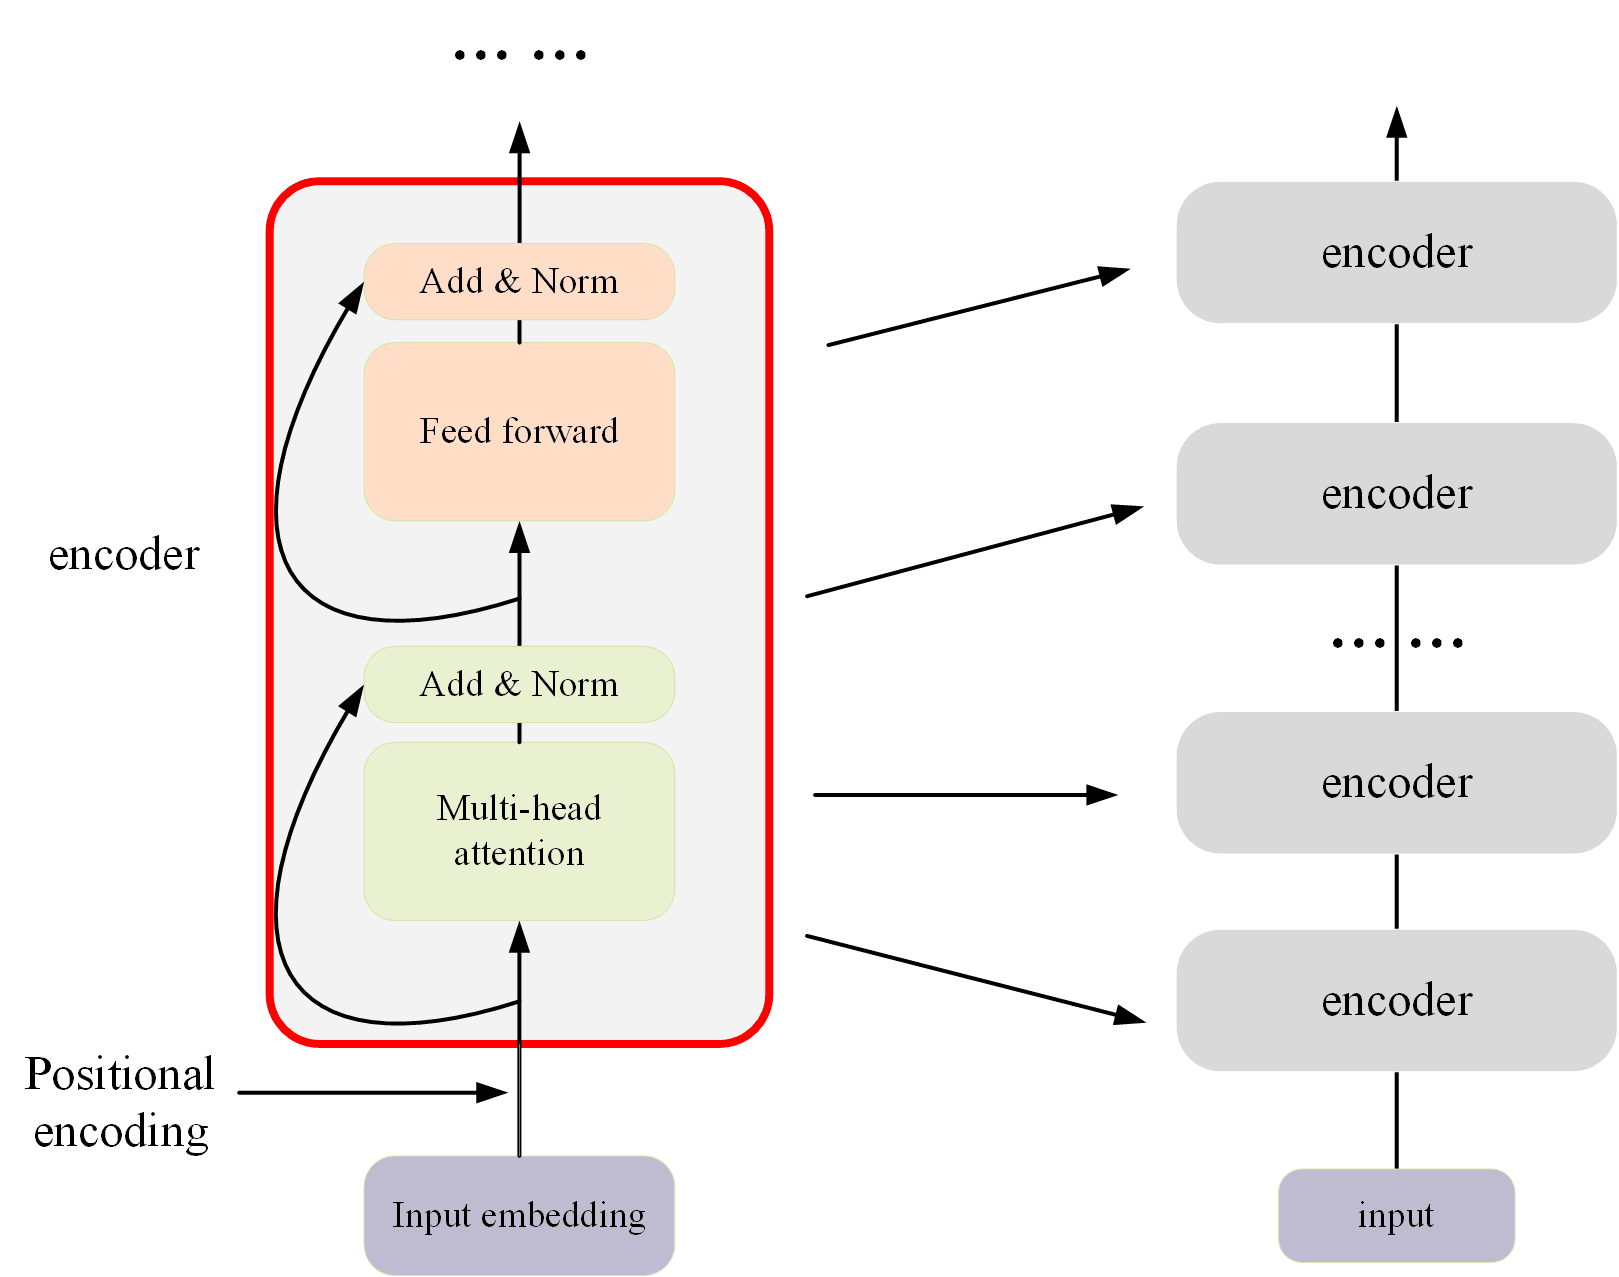
\includegraphics[width=0.8\textwidth]{pic/2-15.png}
	\caption{BERT模型基础架构}
	\label{bert}
\end{figure}
自然语言处理领域的预训练模型。如图\ref{bert}所示,bert主要结构采用了transformer的encoder部分,如图左所示。在每一个encoder结构中,
文本单词向量首先经过一个多头注意力机制以及一个残差连接的标准化层(add \& norm),之后在经过
线性转化和又一个标准化层,将结果输入到下一层网络。如图右所示,bert中由多个这样的encoder结构组成。
BERT预训练过程主要是随机遮盖或替换一句话里面任意字或词,然后让模型通过上下文的理解预测那一个被遮盖或替换的部分。


\chapter{基于图模型的整体文本分类算法}
由前两章介绍可以得知,文本数据由多个单词构成,每个单词可以视作单一的个体,单词之间又充满着联系,因此
采用图模型建模文本数据,有利于分析单词之间的关联,进而有助于提升模型对文本结构、文本蕴意的理解,从而提升
模型分析文本,理解数据的能力。因此,本章提出一个基于图模型理论的方法,将文本数据构建为图结构,从单词之间关联
分析文本内容,实现文本分类任务,提升文本分类准确率。
\section{引言}
近年来,图神经网络被广泛应用于学习图的局部和全局的丰富结构信息\citing{wu2019,zhou2018graph},它引起了众多研究者的极大关注。
文本数据并不是一种天然的图结构数据,需要人为的定义规则去构建图。Yao等人\citing{yao2019graph}就提出了一种基于图模型的文本
分类算法。他们首先根据语料库中词的共现情况以及文档与单词之间共现关系为边,构建了一个包含单词作为节点以及文档也作为节点的图。
然后采用GCN学习单词以及文档节点的向量表示。该方法在测试数据集上展现了良好的性能。但是这个方法忽略了单词在句子中的顺序,同时由于
整个语料库中单词表示仅有一个,忽略了单词在不同语境下可能具有不同的含义,最重要的一点即是构成的图是依据整个语料库构建的单一图,结构
是固定不可更改的,因而图的大小取决于语料库的大小,语料库过大将会导致图模型难以计算,更难以扩展到新的文本数据中。

本章提出一个基于图卷积神经网络(GCN)的文本分类算法。具体来说,该算法为语料库中的每个文本构建一个图,不同于Yao\citing{yao2019graph}的
方法,仅使用单词作为节点,而不考虑文档作为节点。这样有助于捕获词之间在空间、时间和上下文中的信息。
同时算法还为每个图创建一个连接到所有单词节点的“虚拟”超节点,它专门用作上下文感知组件,用于学习文档全局的特定信息。
经过GCN学习后,获得了单词新的向量表示以及一个超结点的向量表示。超结点的向量表示可以视作为文本数据全局信息表示。而对于新的单词向量表示,将其
输入到一个卷积神经网络网络(CNN)用以学习文本数据中局部信息以及序列信息。最终,算法融合超结点向量信息以及CNN模型学到的向量信息,作为
最终的文本向量表示,用以文本分类任务。

综上所述,本研究的主要贡献有两个方面。\noindent\textcircled{1}本章提出了一种基于图模型的文本分类方法,通过单词之间的
关系构建图,通过图模型学习,从而进一步优化单词向量表示。\noindent\textcircled{2} 构建超结点学习文本的全局信息,结合CNN提取出的局部信息
,相比于目前较为常用的方法,模型分类准确率有一定提升。本章第二节对整体文本分类任务问题进行阐述,第三节介绍算法的整体设计,第四、五节
则对模型采用常用的数据集进行验证。

\section{问题定义}
本章主要研究的是对文本数据进行分类的算法。比如一个文本“a very funny movie”,纵观整个句子,从“funny”这个词就能分析出
这句话的情感是正向的,因此整个文本即可归为正向分类。整体文本分类算法是从具体整体含义出发,确定文本所属的某一
类别。

某一文本数据$T_i$由一组$n$个单词构成,$T_i=[w_1,w_2,...,w_{n-1},w_n]$,其中每个单词$w_i$都会有一个初始化的向量$v_i$,
向量可以是随机初始化,也可由各类单词向量表示学习方法获得。因此一个文本可以由一个$\mathbb{R}^{n\times d}$的向量矩阵表示,其中$n$
表示文本中单词的个数,$d$表示为单词向量的维度。文本分类任务就是学得一个函数$F(\cdot)$,通过输入一个文本数据,然后得出该文本所属的类别
,通过一个文本仅对应一个类别。比如根据一段新闻的描述,判断它是属于财经类新闻,还是娱乐明星类的新闻。


\section{算法模型设计}
传统的文本分类算法忽略文本在语料库中整体的统计信息,以及单词之间的互相影响。
因为单词之间互有关联,尤其是同一个句子中的单词含义应该与整个句子的语义有关,而通常的单词嵌入模型每个词向量仅有一种。
因此本章算法采用图模型将单词之间的信息通过图网络互相传递,重新学得更符合整个句子语义的单词的表示。
同时还结合每个单词在整个语料库的统计信息,进一步生成代表整个文本含义的特征向量表示。
对于单词向量继续采用常规的CNN模型进行分析,再与单词统计信息学的到特征向量相结合,最终实现文本分类任务。
本节主要详细介绍算法模型,命名为TextGraph。首先介绍了模型的整体设计,随后详细介绍每一步的具体实现及算法细节。
\subsection{模型总览}
\begin{figure}[htb]%\small tbp
	\setlength{\belowcaptionskip}{0pt}
	\centering
	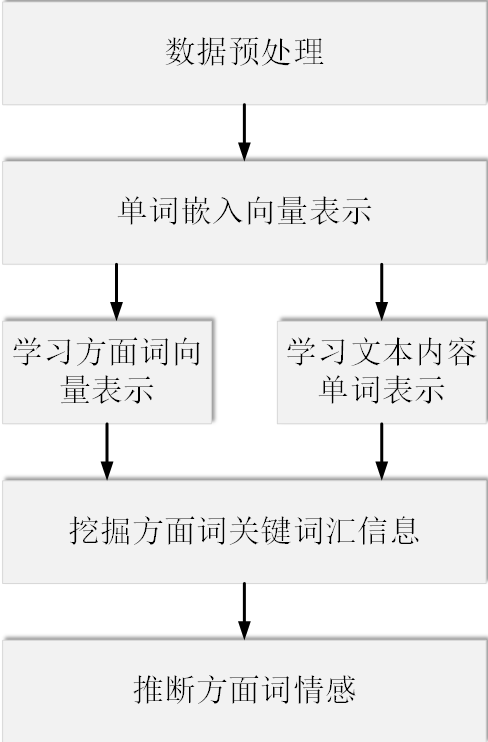
\includegraphics[width=0.3\textwidth]{pic/textgraphLct.png}
	\caption{文本分类算法流程图}
	\label{textgraphLct}
\end{figure}

本章实现的文本分类算法流程如图\ref{textgraphLct}所示。数据预处理主要是指自然语言处理前需要对文本数据进行统一的规则化处理,
比如将所有文本都处理成小写字体,同时删除部分无关的词汇,如一些停止词等。
建立词汇表,不同的单词应该对应一个唯一的索引,有助于后期处理时正确找到每个单词所对应的嵌入向量。
\begin{figure}[htb]%\small tbp
	\setlength{\belowcaptionskip}{0pt}
	\centering
	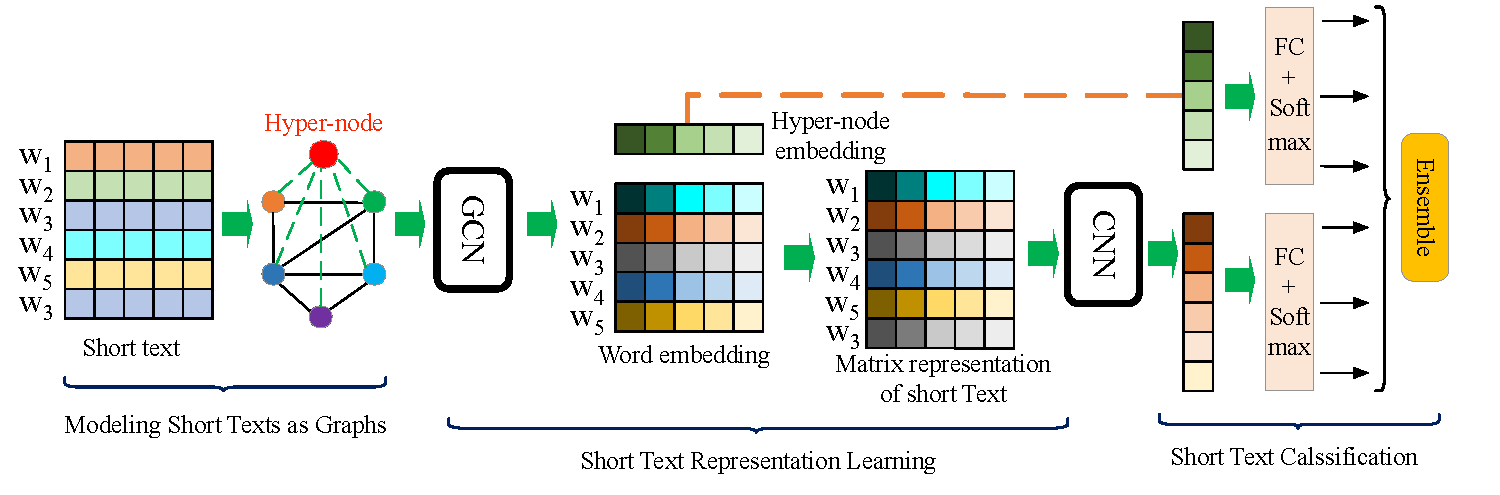
\includegraphics[width=1\textwidth]{pic/TextGraph-arch.pdf}
	\caption{TextGraph模型}
	\label{textGraph}
\end{figure}

TextGraph是一个端到端的模型深度学习模型,输入文本数据,输出文本的标签分类。该算法共有三个部分,如图\ref{textGraph}所示,
第一部分定义为文本构图,即通过一些方法,将文本数据转化为图结构,转化为后面算法计算需要的数据。
第二部分为单词向量表示学习以及CNN网络对文本特征提取,即采用图模型对构成的文本结构图进行学习,获取新的单词向量表示。
对新的向量表示再采用CNN网络提出文本的特征,主要是局部特征。
第三部分为向量信息融合及分类,通过前两步学习,可以获得一个超结点的向量
以及经过CNN池化后的文本向量,两种向量从不同方面学习到了文本的信息,将两类向量进行融合提升模型准确率。以下几节将分别对这些部分
进行详细介绍。
\subsection{文本数据建模为图结构}
TextGraph将文本数据构建为一个带权的有向图,其中每个单词即为一个节点,边表示为单词之间的某种关系。同时,该算法创建了一个超节点,
这个节点连接到所有的单词节点,同时采用特殊的计算方式构建边之间的权重。超结点可以理解为全局信息表示,再模型训练过程中,获取文本的
整体信息,同时将这些信息传递给单词节点,使得单词节点信息表示更加丰富。图中节点的初始化属性即为单词的属性,这类属性通常由单词向量表示学习
方法获得,例如GLove方法\citing{pennington2014glove},有时也可以采用随机初始化的方式表示单词属性,如高斯分布下的随机初始化。

\begin{figure}[htb]
    \setlength{\belowcaptionskip}{0pt}
    \centering
    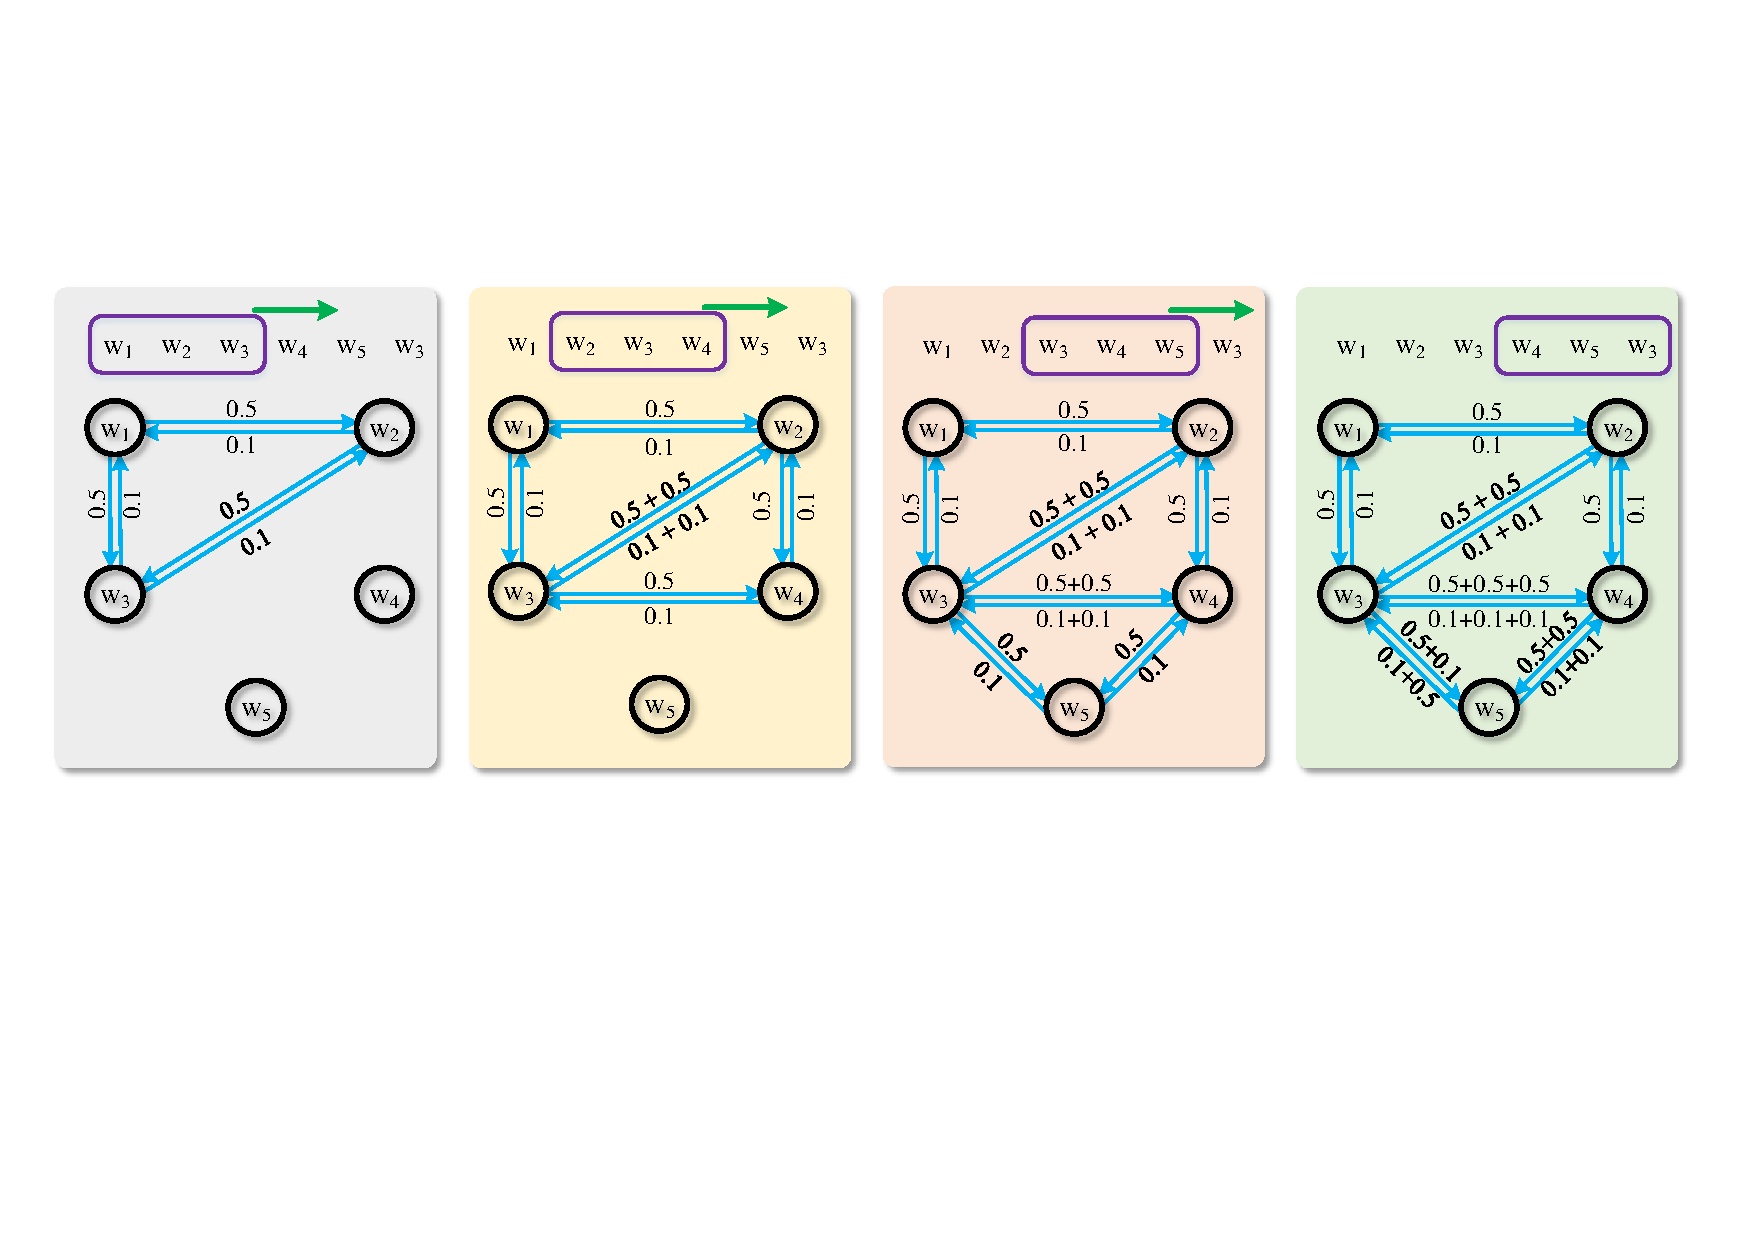
\includegraphics[width=1\textwidth]{pic/text2graph.pdf}
    \caption{图构建过程}
    \label{text2graph}
\end{figure}

为了获得带权重的有向图,该算法采用了滑动窗口策略实现。滑动窗口的大小$m$是固定的,主要根据实验结果获得。该策略详细步骤如下。
滑动窗口是对文本的单词进行滑动,每个窗口内根据窗口大小$m$,包含$m$个单词。在窗口中,单词与单词之间构成一个单词对,前一个单词对于后一个单词具有
权重$w_f$,后一个对于前一个单词具有权重$w_b$,其中$w_f$和$w_b$也是预先定义的固定大小的值,为了反映序列信息,通常这两个值不一样。
因此滑动窗口大小$m$和权重$w_f$和$w_b$是可调节的超参数。滑动窗口依次从左向右移动一个单词距离。如果已经存在连接两个单词的边,则将累积相应的权重。
这个过程不断迭代,直到滑动窗口覆盖了文本的最后一个单词。如图\ref{text2graph}所示,给定的文本序列是$[w_1,w_2,w_3,w_4,w_5,w_3]$,其中每个$w_i$是一个单词。
为了简单起见,将参数设置为$m=3$、$w_f=0.5$和$w_b=0.1$。开始时,滑动窗口覆盖$[w_1,w_2,w_3]$这三个单词,因此构成了
前向边$(w_1,w_2)$,$(w_1,w_3)$,和$(w_2,w_3)$,每个权重均为0.5。同时,后向边有$(w_2,w_1)$,$(w_3,w_1)$,和$(w_3,w_2)$,其权重为0.1。
然后,滑动窗口向右移动一个单词,到达$[w_2,w_3,w_4]$这个序列。由于边$(w_2,w_3)$已经存在,新的权重将变为$0.5+0.5$。
同样,对于边$(w_3,w_2)$,新的权重变为$0.1+0.1$。此过程一直持续到最后一个窗口$[w_4,w_5,w_3]$。单词$i$和单词$j$之间的累计权重由$a{ij}$表示,
该算法通过滑动窗口的总数来规范化$a{ij}$,计算方式为$\frac{a{ij}}{c}$,其中$c$为滑动窗口次数。超结点则是连接到所有其他单词节点的一个虚拟节点,其
边的权重由整个语料库中单词的TF-IDF计算得到。因此节点与节点之间的权重$A_{ij}$可以由公式\ref{weightGraph}得到。
\begin{equation}\label{weightGraph}
A_{ij}=
\begin{cases}
\frac{a_{ij}}{c}& \text{当 $i, j$ 都是单词时}\\
TF\text{-}IDF(i) & \text{当$i$ 是单词, $j$ 是超结点时}\\
1 & \text{$i=j$}\\
0 & \text{其他情况}
\end{cases}
\end{equation}

因此,对于图\ref{text2graph}中的文本的邻接矩阵$A$可以如下公式\ref{adjacentmatrix}表示,该矩阵不包含超结点的权重信息。
\begin{equation}
    \label{adjacentmatrix}
    A=\left[
    {\begin{array}{*{20}{c}}
     {\text{1}}&{{\text{0}}{\text{.5/4}}}&{{\text{0}}{\text{.5/4}}}&{\text{0}}&{\text{0}} \\
     {{\text{0}}{\text{.1/4}}}&{\text{1}}&{\text{1/4}}&{{\text{0}}{\text{.5/4}}}&{\text{0}} \\
     {{\text{0}}{\text{.1/4}}}&{{\text{0}}{\text{.2/4}}}&{\text{1}}&{{\text{1}}{\text{.5/4}}}&{{\text{0}}{\text{.6/4}}} \\
     {\text{0}}&{{\text{0}}{\text{.1/4}}}&{{\text{0}}{\text{.3/4}}}&{\text{1}}&{\text{1/4}} \\
     {\text{0}}&{\text{0}}&{{\text{0}}{\text{.6/4}}}&{{\text{0}}{\text{.2/4}}}&{\text{1}}
    \end{array}}
    \right]
    \end{equation}

\subsection{表示学习过程}
文本分类效果取决于单词嵌入表示的学习以及文本表示学习过程,TextGraph通过GCN网络重新学习到单词向量表示,
再将学习到的向量表示输入到CNN网络结构中进一步提取特征信息,以达到最优的特征提取。

本章采用GCN网络去学习构建好的文本图数据。通过多层的GCN,单词节点不仅能够获取与自己在同一窗口下的其他单词信息,
也能获取得到得更远的单词信息。单词之间的信息可以通过构建好的边进行共享。而对于超结点,因为包含了语料库中
单词的共现信息——通过TF-IDF方法获得到的,因此超结点在GCN网络学习的过程中,会获得整个文本的全局信息,同时这些信息
也会选择性的传递给所有单词节点,以辅助单词节点学习到更加丰富的表示。同时,采用了注意力机制辅助模型在学习的过程中关注于
重点信息。即有些单词之间虽然具有边,但是由于这些单词之间关联程度并不高,采用注意力机制有助于降低对不重要信息的关注,
将更多注意力放在重点的单词节点上进行信息传递。因此对于单词$i$,$j$之间的注意力分数可以通过公式\ref{textGraphAttFor}得到。
\begin{equation}\label{textGraphAttFor}
    \gamma_{ij}=sigmoid(x_iW_{a1})+sigmoid(x_jW_{a2})
\end{equation}

$\gamma_{ij}$即为注意力分数,其中$W_{a1}$和$W_{a2}$为$d\times 1$的权重矩阵,$x_i$,$x_j$为当前单词$i,j$的向量表示,
为$1\times d$的向量。$sigmoid$为激活函数。加入注意力机制后,与形如公式\ref{GNNFormula1}所示的GCN计算方式略
有不同,对于每一层的单词向量表示计算可以由公式\ref{textGraphLayerFor},\ref{A_hat},\ref{D_hat}计算得到。
\begin{equation}\label{textGraphLayerFor}
    H^l=\sigma((\gamma ^l\hat{D}^{-\frac{1}{2}}\hat{A}\hat{D}^{-\frac{1}{2}})H^{l-1}W^l)
\end{equation}
\begin{equation}\label{A_hat}
    \hat{A} = A+I
\end{equation}
\begin{equation}\label{D_hat}
    \hat{D} = \sum{j}A_{ij}
\end{equation}
其中$H^l$为$n*d$的矩阵,第$i$行的向量表示为文本序列中第$i$个单词的在GCN网络中第$l$层的向量表示,为一个$1\times d$的向量。
$\gamma ^l$则为第$l$层计算得到的权重矩阵。

经过GCN网络学习后,每一单词向量都得到更新,获得了新的向量表示,假设第$i$个单词的输出向量为$h_i\in \mathbb{R}^k$,其是一个、
$k$维的单词向量。因此对于一个包含$n$个单词的文本序列可以获得一个$H\in \mathbb{R}^{n\times k}$的矩阵,即$H=[h_1, h_2,\cdots, h_n]^T$。

为了得到文本的局部信息以及序列信息,本算法采用一个一维卷积神经网络(CNN)结构提取相关特征。
其中CNN网络中的卷积核$\mathbf{w} \in \mathbb{R}^{h\times k}$是一个$h \times k$的权重矩阵,
$h$表示为当前CNN网络的卷积窗口大小为$h$,即每次窗口考虑$h$个单词用以计算特征值,计算公式如\ref{cnnFor}所示。其中$\sigma$
是一个激活函数,$b$是偏置矩阵。
\begin{equation}\label{cnnFor}
    f_i=\sigma(\mathbf{w} \cdot y_{i:i+h}+b)
\end{equation}

文本数据的卷积操作不同于图像数据,只会在文本序列的一个方向做卷积,即在垂直方向做卷积。卷积核每次移动向下一个单词移动一次,如图\ref{cnnslide}所示,红色线框为卷积核,每次计算
生成一个特征值,之后向下移动一步,如虚线框所示。因此这样的卷积操作下,将会生成$(n-h+1)$个特征值。
\begin{figure}[htb]
    \setlength{\belowcaptionskip}{0pt}
    \centering
    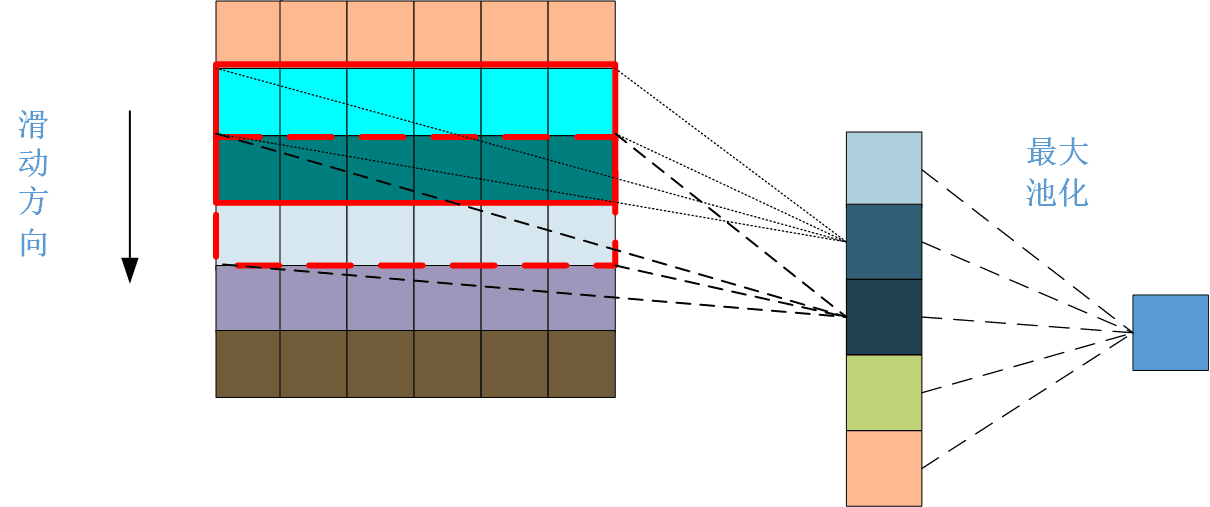
\includegraphics[width=0.6\textwidth]{pic/cnnslide.png}
    \caption{CNN特征生成过程}
    \label{cnnslide}
\end{figure}

对于每一个卷积核产生的一组特征值,为了获取其中最关键的特征,本算法采用最大池化操作进行特征提取。
最大池化操作有助于选取最重要的特征,比如一句话“这个公园景色不错,但是我今天玩得并不开心。”,虽然这句话
从前面的信息来看好像是正面的表述,实际上通观全文,最后的“玩得并不开心”的信息才是最重要的。
通过选择每个卷积核中的提取的特征的最大值,可捕获其最重要的特征。这样操作后每一个卷积核得到特征就是一个值。
另一方面,采用池化操作有助于降低参数量,进而可以减少模型过拟合问题。经过多个卷积核的卷积池化操作后,将这些所有卷积核产生
的特征值拼接起来就能得到文本的特性向量表示。

\subsection{向量融合及分类}
经过以上步骤,将获得一个超结点的向量表示$e_h$,这个向量可以理解为对全局信息的捕捉;以及经过CNN网络提取得到的文本向量表示$e_c$,
这个向量可以理解为对局部信息以及重点关注信息的表示。总之,这两个向量都可以作为文本的向量表示,只是包含的信息内容有所不同。
$e_h$和$e_c$都可以单独作为结果实现文本分类。而两者的结合将会获得表示更加充分的文本向量。

本章,采用两个不同的线性变化层,将$e_h$和$e_c$向量转为为与标签大小$m$同一维度,如公式\ref{eh1},\ref{et1}所示。
\begin{equation}\label{eh1}
    s_h=softmax(e_h \cdot \mathbf{w}_{f1}+b_1)
\end{equation}
\begin{equation}\label{et1}
    s_c=softmax(e_c \cdot \mathbf{w}_{f2}+b_2)
\end{equation}

其中$w_{f1}\in \mathbb{R}^{d_1 \times m}$为$d_1\times m$的参数矩阵,$w_{f2}\in \mathbb{R}^{d_2 \times m}$
为$d_2\times m$的参数矩阵.$d_1$、$d_2$分别为$e_h$和$e_t$的维度大小。softmax为激活函数,是将一组数值压缩到0-1之间,它们的和为1,
可以近似的看做是预测概率。对于分类任务而言,一个$1\times m$的输出向量经过softmax计算后,每一位置上的值
可视作这个位置上对应的标签的概率。softmax计算如公式\ref{softmax}所示。
\begin{equation}\label{softmax}
    s=\frac{e_i}{\sum{j}{e_j}}
\end{equation}

经过以上公式计算得到了来至于超结点的预测结果$s_h$以及来自CNN的预测结果$s_c$。为了平衡两者预测的影响,本节采用了一个
超参数$\alpha$去控制,如公式\ref{output}所示。$\alpha$ 取值在0-1之间。
\begin{equation}\label{output}
    O=(1-\alpha) \times s_h+\alpha \times s_c
\end{equation}

因此对于整个模型来说代价函数$C$可以由公式\ref{costFun}得出。
\begin{equation}\label{costFun}
    C=-\frac{1}{M}\sum \limits_{x}\left[(1-\alpha)(ylna_h+(1-y)ln(1-a_h)+\alpha(ylna_c+(1-y)ln(1-a_c)\right]
\end{equation}

其中$M$表示为所有样本数,$x$代表一个样本,$y$表示当前这个样本的真实标签,$a_h$表示为超结点向量
最终的预测结果,$a_c$表示为CNN提取的文本向量最后的预测结果。

\section{实验设置}
\subsection{数据集描述及数据处理}
本章使用文本分类任务中广泛使用的一些数据集,其中包括R8、R52、MR、Yelp等数据集。本章分别在这四种数据集上进行验证模型及与其他模型进行对比。

\textbf{R8和R52}数据集是广泛被使用的一种用于文本分类任务的数据集,其主要来至于路透社的新闻数据。因此其为英文文本数据集。
对于R52来说总共有6532个训练集样本以及2568个测试集样本,平均文本长度为69.82,共计52种分类类别。R8数据集共计有5485样本用做训练集,
2189个样本用作测试集,平均文本长度65.72,共计8个不同的类别标签。
以R8数据集为例,其文本数据如“us house speaker wright concerned of interest rate rise under greenspan ”,该文本数据对应的标签为“interest”,即对于R8数据集
来说,是对文本数据打上最符合的8种标签中的一个。

\textbf{MR}\citing{pang2005seeing}数据集是一种在每个文本序列中只包含一种情感的电影评论数据集。它包括5331个负面情感数据样本以及5331个正面情感的样本,其平均长度为20.39。
本章中采用Tang等人\citing{tang2015pte}使用的训练集测试集划分方式。
MR数据集中数据如“the cast is phenomenal , especially the women”所示,其中这个文本对应的标签为“1”,即代表为正面情感。MR总共两种情感,数据集中分别
用“0”,“1”分别表示负面情感和正面情感。

\textbf{Yelp}也是一种评论数据集,其标签是1-5之间的分数,共计5种标签。为了平衡数据集划分以及控制文本数据集的长度,
本章对这类数据集中的所有数据进行随机抽取,仅抽取文本长度在150个以下的,最终共计获得18972个数据集样本,其中包含14000个用作训练集,4972个用作测试集,
同时将平均文本长度在81.17。
取其中一个文本为例,Yelp数据集文本如“awesome mall all kinds of stores we dont have on the west side ! !”,这段文本对应的标签为“4”,即对于Yelp数据集来说,
每个文本都有一个在1-5之间的标签。

以上四种数据集详细统计如表\ref{summary}所示。

\begin{table*}[htb]
	\centering
	\caption{数据集数据统计}
	\setlength{\tabcolsep}{0.7mm}{
		\begin{tabular}{c|c|c|c|c|c|c}
			\hline 
			{数据集} & {总文本数} & {训练集数}& {测试集数} & {单词数} & {类别数}& {平均长度}  \\
			\hline 
			$ \text{R8} $ & $ 7,674 $ & $ 5,485 $& $ 2,189 $ & $ 7,688 $ & $ 8 $ & $ 65.72 $ \\ \hline
			$ \text{R52} $& $ 9,100 $& $ 6,532 $ & $ 2,568 $ & $ 2,568 $& $ 52 $& $ 69.82 $  \\\hline
            $ \text{MR} $&$ 10,662 $& $ 7,108 $& $ 3,554 $ & $ 18,764 $ &$ 2 $& $ 20.39 $ \\\hline 
            $ \text{Yelp} $&$ 18,972 $& $ 14,000 $& $ 4972 $ & $ 26,889 $ &$ 5 $& $ 81.17 $ \\\hline 
		\end{tabular}%
		\label{summary}%
	}
\end{table*}

本章中使用的均为英文数据集,因此不用考虑像中文分词。由于英文单词有大小写之分,例如希望在文本处理过程中将“No”和“no”
视作是一个词,因此一般需要将所有的词都转化为小写。同时在文本中存在一些停用词,即许多对分类任务没有太大帮助的词语,比如“aha”、“oh”等,
因此也将这些词语去掉。如句子“No one wants to see this movie. Oh, it's too bad” 经过预处理后变为“
no one wants to see this movie. it's too bad”。对自然语言的文本数据,计算机是无法直接理解的,需要将其转化为计算机能够识别的数据。
本章使用Glove作为词向量初始化输入。首先对于一个句子,采用“空格”作为分割,将一句话转化为单词列表,如上句子转为单词列表即为
\centerline{$[no,one,wants,to,see,this,movie,it's,too,bad]$}

同时根据整个语料库对所有的单词进行一个唯一编号,本章根据单词出现的顺序进行编号,每个单词
均有一个数字作为唯一标识,如上句单词列表经过编号转化后,可能表示如下:

\centerline{$[4,487,3667,34,1,555,676,12465,376,89]$}

每个编号同时还对应着一个维度为300的唯一的向量表示,来自于Glove。例如单词“no”在glove中的向量表示如下:


\centerline{[-0.015103  -0.618705  0.127657  0.020094  0.186504 }

\centerline{...}

\centerline{0.032921  -0.153918  0.827338  -0.409457]}

也即是编号“4”对应的向量如上。例如对于一个单词数量为18764的MR数据集,便有18764个对应的词向量。如果词向量不存在于Glove
中,则采用随机初始化的方式生成。因此上述句子便能转为一个形如下的向量矩阵:

\centerline{[-0.015103  -0.618705  0.127657  0.020094  0.186504 }

\centerline{...}

\centerline{0.032921  -0.153918  0.827338  -0.409457]}

\centerline{[0.115103  -0.612235  0.432126  0.045531  -0.488512 }

\centerline{...}

\centerline{-0.132921  0.148618  0.395361  0.642315]}

\centerline{...}

\centerline{[0.515103  -0.122212  0.007217  0.123204  -0.076414 }

\centerline{...}

\centerline{0.102212  -0.000123  0.464318  0.100671]}

最后这样的一个单词矩阵就可以作为计算机可以识别的输入。
\subsection{对比方法介绍}
本章提出的方法是用于实现整体文本分类任务,即一个文本对应一个标签类。因此,所对比的方法都是用于该文本分类任务,且均采用
Glove词向量作为单词的初始化向量。所涉及的比较方法均属于深度学习模型,且是目前广泛使用的自然语言处理模型。比较模型主要包括以下:

\textbf{LSTM:} 是一种特殊的RNN模型,可以解决长序列训练过程中的梯度消失和梯度爆炸问题,相比于普通的RNN模型,具有更优异的表现。
LSTM每一个循环中,对于输入的单词向量均会产生一个隐藏向量表示,本章中将这些生成的单词的隐藏向量表示做一个平均池化作为文本的向量,
用于实现文本分类任务。

\textbf{Bi-LSTM:}\citing{schuster1997bidirectional} 是一种双向的LSTM模型。它将一个句子从前到后进行处理,同时对句子从后到前进行编码,最后将
两种信息拼接起来。相比于LSTM多了一个从后到前的信息,这样的设计有利于模型进行更细粒度的理解,更好的捕捉双向的语义依赖。本章中采用LSTM获取文本
向量的方式,对通过前向LSTM获得到的文本向量以及从后向LSTM获取的到的文本向量进行拼接,作为最终的文本向量表示,以用于分类任务。

\textbf{TextGCN:}
\subsection{模型训练及参数设置}
\subsection{实验评价指标}

\section{实验结果及分析}

\chapter{基于图模型的方面级情感分析算法}
第三章探讨了基于图模型理论的整体文本分类算法,图模型应用于文本分类任务取得了一定效果。尤其是考虑作为全局信息而引入的超节点
对模型性能有一定的正面影响。超节点实际上不仅仅可以作为全局信息而使用,根据不同任务可以设置不同类型的超节点。本章依旧基于图模型
理论,探讨关于方面级情感分析的任务。本章算法超节点不再使用全局信息而使用方面词信息,并与第三章构图方式一致,建立文本图结构,实现方面级
情感分析。

\section{引言}
方面级情感分类\citing{zhou2019deep}已经越来越备受关注,相比于一般的文本分类算法具有更高的实用性。例如对于在美团、京东、天猫等平台上进行的商品评价描述,
采用方面级的情感分类可以针对商品不同的方面进行评价,进而实现对产品全方位的点评,并且平台可以根据点评的方面以于分类,以保障用户对不同方面的感知和需求。
比如有些用户看重服务,有些用户看重质量。同时商家可以根据用户对不同方面的评价进行改进,提升商品整体质量。方面级情感分类相比于一般的文本分类算法,具有一定难度。

Li等人\citing{li2018transformation}使用一个Bi-LSTM模型处理文本序列,获取每个单词的中间隐藏状态的向量表示,随后每个单词向量对应一个CPT结构(Context-Preserving Transformation)。
每个CPT中采用Bi-LSTM模型学习一个方面词对应的信息向量然后与输入的单词向量拼接获取一个新的单词向量,该向量体现了每个单词与目标词之间的关系信息。
通过CPT层后,每个单词具有一个新的向量表示,再对这组向量表示采用CNN模型卷积处理,捕捉关键信息,生成表示文本的向量,用以实现分类。
Wang等人\citing{wang2016attention}提出了一个基于LSTM的注意力机制模型。它将方面词的向量表示分别与文本内容的每个单词向量表示进行拼接,组合成新的向量,作为LSTM模型的输入。
随后将LSTM模型获得的每步单词的隐藏状态与方面词向量用一个注意力机制求得权重,代表了每个单词对目标情感的贡献度。最后通过向量加权和表示最终的用以分类的向量表示。虽然
这些方法取得了一定效果,但是使用不能并行计算的LSTM模型,计算效率相对较低。同时方面级的目标词与文本内容单词之间应该存在许多联系,
如果能够挖掘它们之间的内在关系,便能进一步学到情感信息。

本章基于第三章提出的图模型算法,进一步改进使之适合方面级情感分析任务。具体来说,本章的算法不再使用依据语料库信息构建超节点,而是使用对应的方面词构建,即希望这个超节点学习到的
是方面词信息,同时将这个信息通过图结构传递给其他单词节点。文本图其他部分构建过程采用第三章描述的方式一致。考虑到门控机制具有选择遗忘的功能,而图卷积神经网络
每一层的节点信息对于下一层并不一定都有用,因此,本章采用一个门控机制去控制每层节点信息的流动。通过图模型学习,将获得每个单词新的向量表示以及一个表示为方面词的信息向量。
方面词的具体情感信息取决于文本中对应位置的情感词汇,因此,本章继续采用一个注意力机制,通过方面词向量去查询所有单词中对它情感偏向最重要的词汇,获得相应的权重,最后将这些向量进行
加权和,得到最终的用以实现分类任务的向量。

综上所示,本章提出的方法主要有以下三点特色:\noindent\textcircled{1}采用一个超节点表示方面词信息,并将这个信息通过图网络进行传递,进而捕捉文本单词以及方面词之间的关系,学到两者的向量表示。
\noindent\textcircled{2}通过门控机制选择或遗忘传递给图模型中下一层的信息。\noindent\textcircled{3}利用注意力机制寻找对目标词情感贡献最大的词汇。

\section{问题定义}
本章主要探讨的是方面级情感分类任务。对于这类任务不同于整体文本分类任务,每个文本中都有一个或多个方面词。如句子“great food but the service was dreadful”,这个句子中定义
了两个方面词一个是“food”,另一个是“service”,方面级情感分类任务的目标就是判断这两个方面词对应的情感倾向。如“food”这个词,采用“great”进行形容,是一个褒义词,因此对于“food”的情感
可以归属于正向的。而对于“service”这个词,是使用“dreadful”进行描述的,属于贬义词,因此情感归属于负面。

某一文本数据$T_i$由一组$n$个单词以及多个方面词构成,$T_i=[w_1,a_{i}...a_{j},w_{n-1},w_n]$。其中$w$表示一个单词,$a_i$表示为第$i$个方面词,通常方面词由一个或多个单词组成。
文本中每个单词都有一个对应的单词向量,本章采用的单词向量主要是从Glove或经过BERT模型后得到。因此一个文本可以由一个$\mathbb{R}^{n\times d}$的向量矩阵表示,其中$n$
表示文本中单词的个数,$d$表示为单词向量的维度。方面级情感分类任务就是学得一个函数$F(\cdot)$,输入这段文本以及需要分析的这段文本中的方面词,输出这个方面词对应的情感倾向,即判断
这个方面词是正向的或是负面的或是无情感。

\section{算法模型设计}
以前的一些研究仅仅直接对方面词的向量以及文本向量进行拼接,并未细致考虑方面词与文本中其他单词之间的联系。如果能够挖掘它们之间的内在关系,便能进一步提升模型性能。此外在图卷积网络计算中
,网络层数的增加意味着当前节点将会获取得到更远处节点的信息。而更远处节点的信息不一定对当前节点有用,因此本章采用一个门控机制,选择性的选择或是遗忘节点信息,控制信息流动,进一步提升模型
性能,确保学到更有效的向量表示。注意力机制使得模型关注于重要信息,查找对于方面词情感分析更为重要的词汇。本节主要详细阐述了算法模型,命名为GAGCN,首先介绍了模型的整体设计,之后再详细介绍
每一步的具体实现。

\subsection{模型总览}
本章实现的方面级情感分析算法流程图如图\ref{asgraphLct}所示。预处理是指对文本数据进行统一的规则化处理,首先将所有文本都处理成小写字体,同时删除部分无关的词汇,比如一些停止词等。
建立词汇表,不同的单词应该对应一个唯一的索引,有助于后期处理时正确找到每个单词所对应的嵌入向量。同时需要标注每个文本中对应的方面词所在位置,便于后续分析任务使用。
\begin{figure}[htb]
	\setlength{\belowcaptionskip}{0pt}
	\centering
	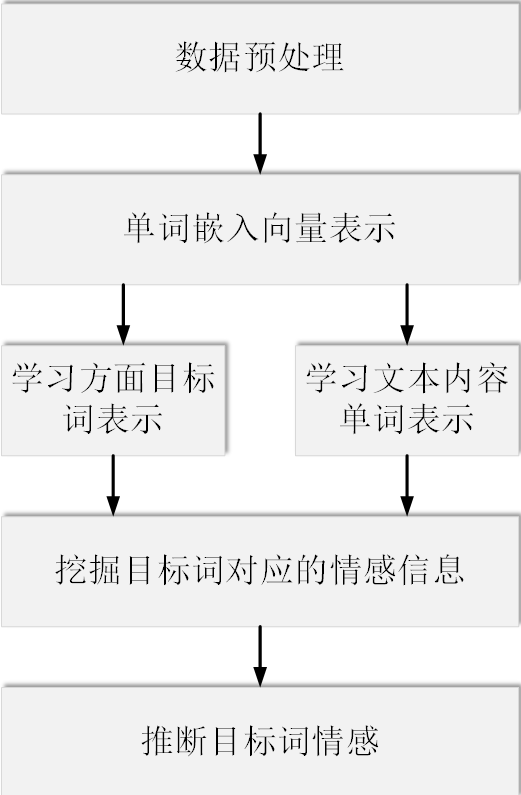
\includegraphics[width=0.3\textwidth]{pic/asgraph.png}
	\caption{方面级情感分析算法流程图}
	\label{asgraphLct}
\end{figure}
方面词向量以及文本单词向量的学习都是基于图网络模型,经过图卷积神经网络学得到一个超节点向量,即表示为方面词向量,以及每个单词的新的向量表示。方面词关键词汇信息挖掘即是使用注意力机制
关注重点词汇,找出对该方面词的情感倾向有帮助的词汇,最后实现分析。

本章提出的方法是一个端到端的深度学习模型,即输入文本内容和对应的方面词,就可得到该方面词对应的情感类别。该算法总共有三个部分,如图\ref{asgraphart}所示,第一部分定义为文本构图部分,
该步骤主要是将文本中的单词采用第三章提到的构图方法构建成图,其次构造一个传递方面词信息的超节点。第二部分主要是单词词向量表示学习以及超节点的表示学习,这部分采用基于多头注意力机制的GCN
进行学习以及一个门控机制用以控制图网络模型中每一层信息的传递。第三部分是基于第二部分学到的文本词向量以及超节点向量来计算。将超节点向量作为注意力机制中的Query向量,
计算文本单词中所有单词的权重,权重的大小即可视作这个单词对方面词情感的分析的重要程度。随后将注意力机制获得向量与超节点向量进行一个简单地结合,即得到最终的分类向量,将这个向量输入一个简单的
神经网络通过softmax激活函数实现情感分析任务。以下几节将对这些部分进行详细介绍。
\begin{figure}[htb]
	\setlength{\belowcaptionskip}{0pt}
	\centering
	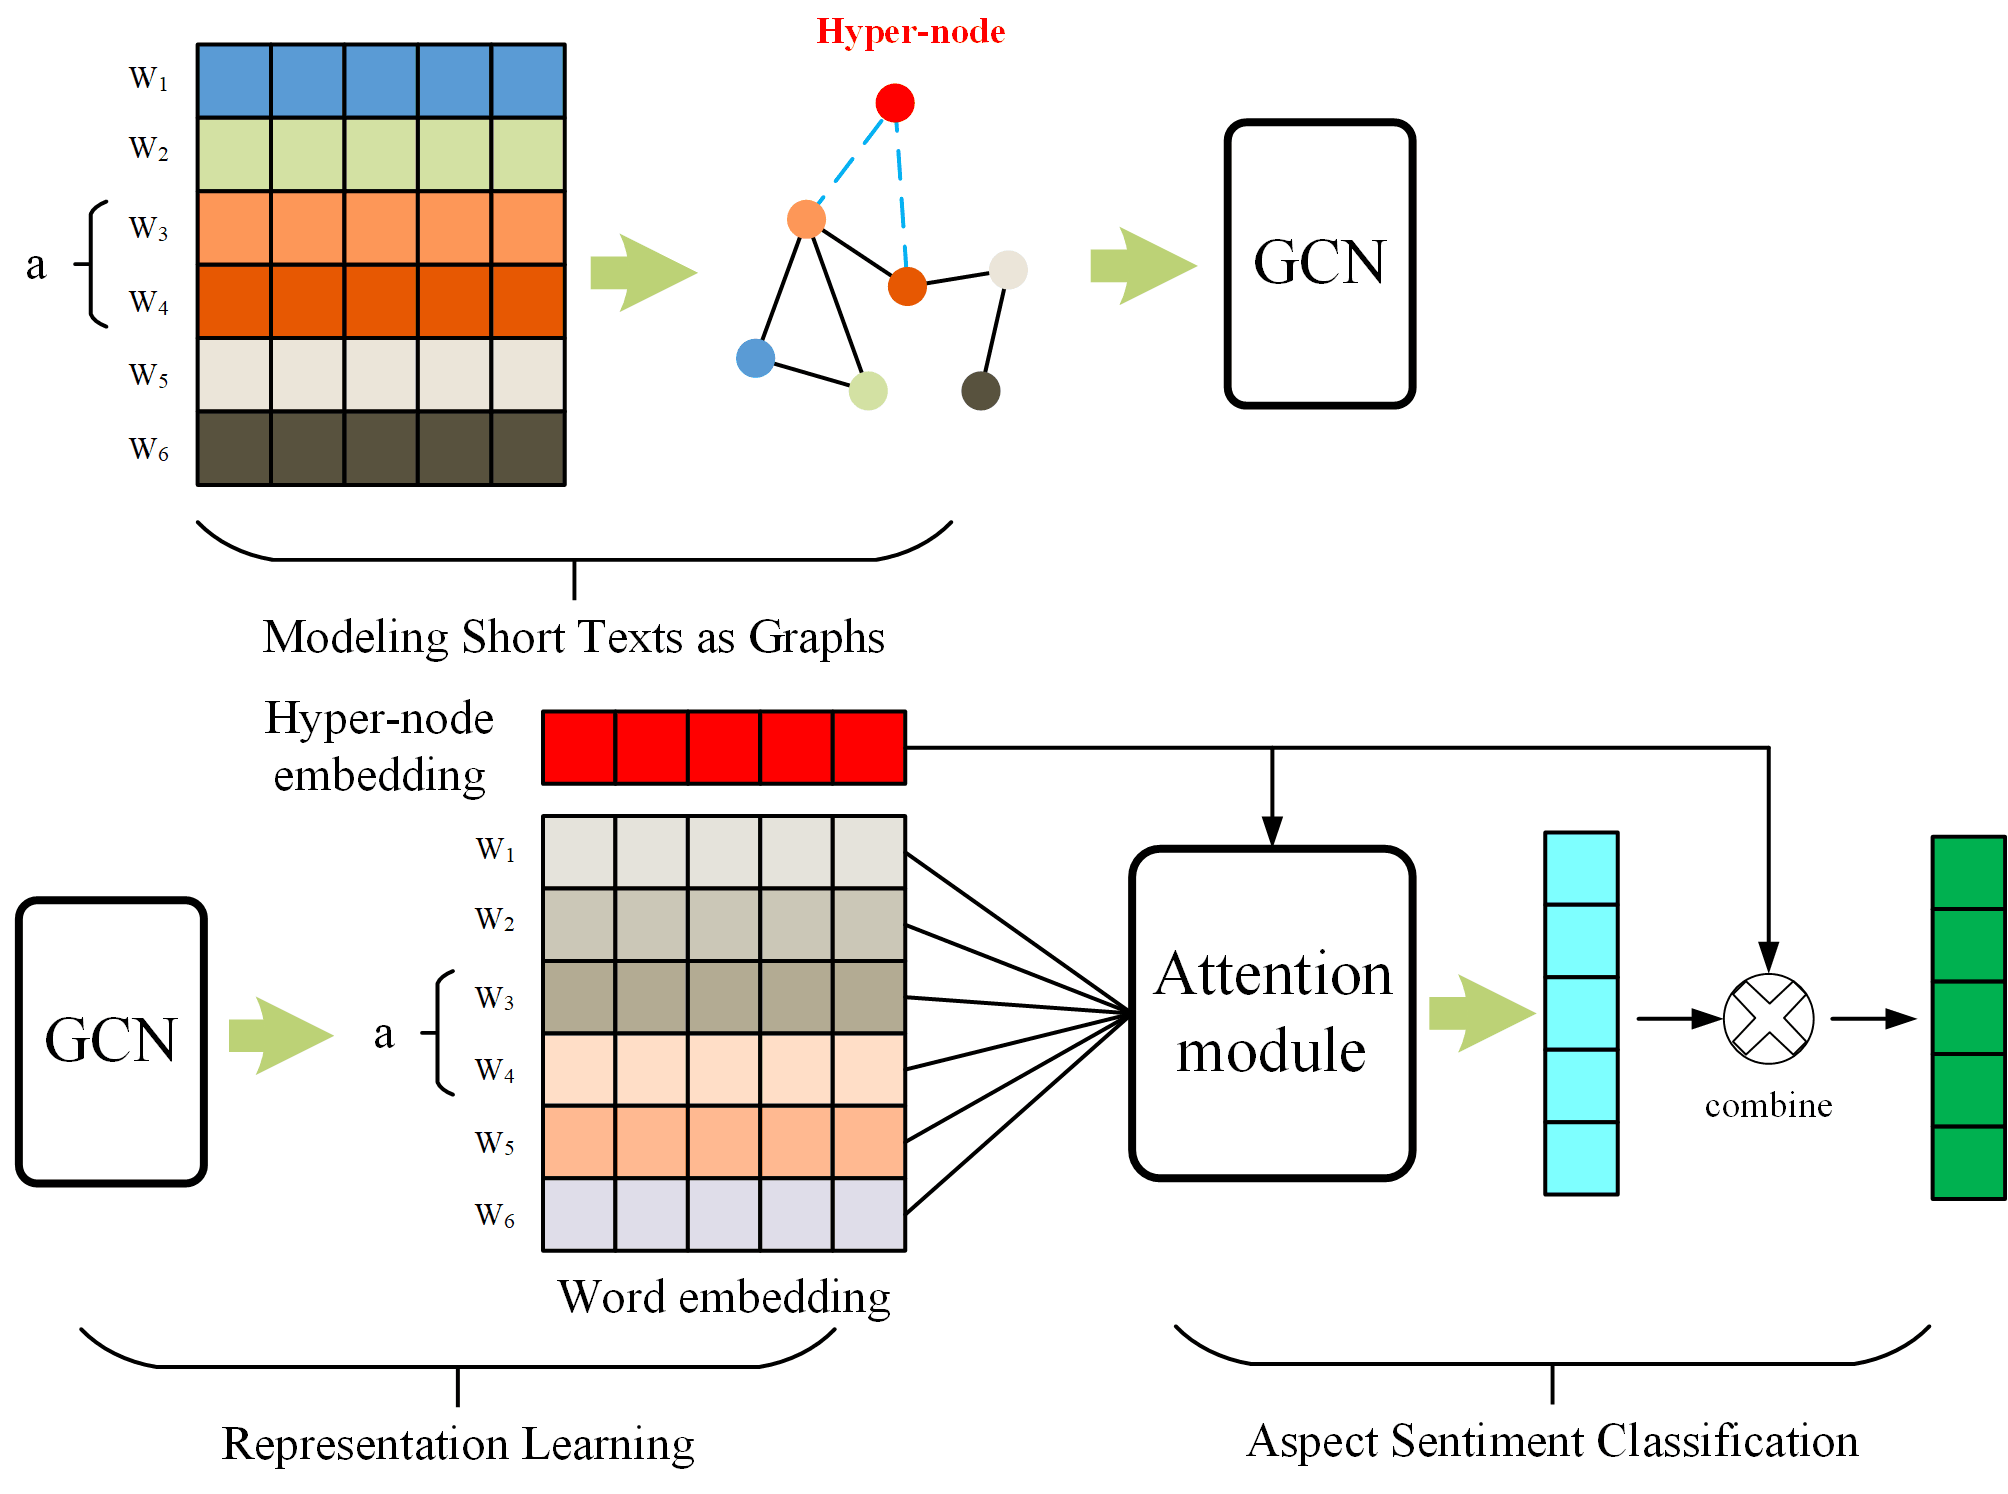
\includegraphics[width=1\textwidth]{pic/asgraphart.png}
	\caption{方面级情感分析算法模型}
	\label{asgraphart}
\end{figure}

\subsection{文本图建模过程}
本章文本图的构建过程与第三章图构建过程一致,均是采用滑动窗口的方式构建单词与单词之间的图。但与第三章略有不同,第三章中每个单词在图中仅有一个节点,即使一个单词在同一个文本中只出现了一次,
也仅仅视作一个节点。而本章中因为同时还要采用BERT预训练模型,因此构图过程中,为文本中每一个单词都构建一个节点,即使是同一个单词只要出现的位置不同,均构建一个不同的节点。单词与单词之间的边如
第三章公式\ref{weightGraph}所示。超节点不再使用TF-IDF的方式计算,构建的超节点依然是一个双向边,一向由方面词节点连向超节点,一向由超节点连接方面词。如图\ref{asgraphart}所示,图中$w_3$$w_4$是
属于方面词$a$的两个单词,超节点分别构建一条连接这两个单词节点的边,如图中虚线所示。构建时边的权重为固定值1,在图卷积计算过程中会由注意力机制更新权重,着重关注于方面词中重要的词汇。
超节点中双向边的构建有助于超节点向量传递给方面词中的每个单词,超节点向量可以视作整个方面词的信息,通过把完整的信息传递给其中的每个单词节点,有助于方面词中单词信息理解的完整度。其次,在多层的图卷积
过程中,超节点信息也能进一步传递给其他单词节点,使得其他节点也能获得方面词向量信息。这样有助于整个文本向量理解任务目标,明确需要分类的具体方面词,进而有目的性的去学习有用的词向量。


\subsection{词向量与超节点向量表示学习}
表示学习过程依然采用图卷积神经网络进行。相比于第三章提出的方法,在注意力机制计算过程进行了改进,同时还提出一个门控机制对每层传递的信息进行控制。如图\ref{attgcn}所示,假设在
每一层GCN网络中,当前需要计算的
\begin{figure}[htb]
	\setlength{\belowcaptionskip}{0pt}
	\centering
	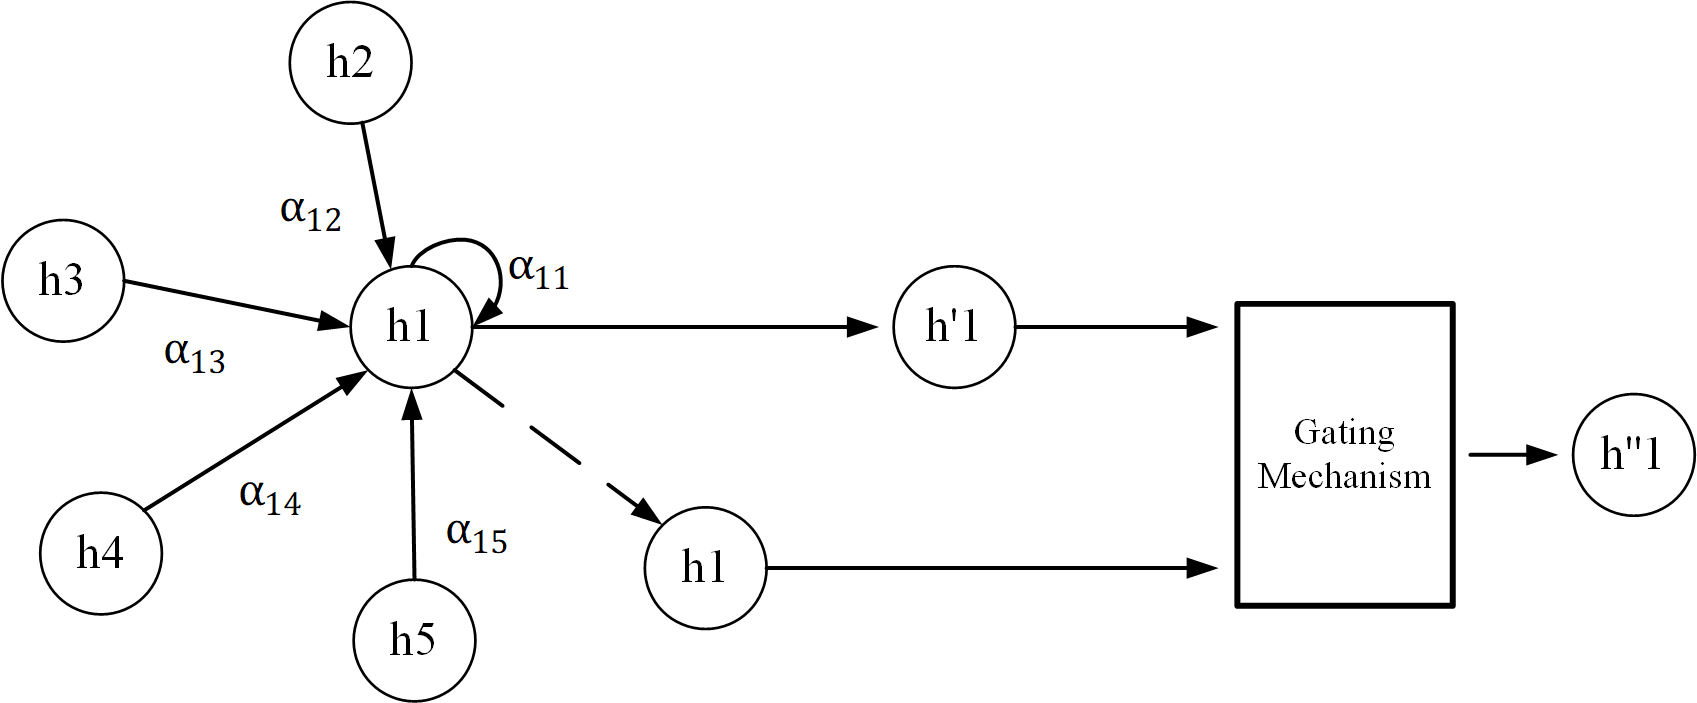
\includegraphics[width=1\textwidth]{pic/attgcn.png}
	\caption{方面级情感分析算法模型}
	\label{attgcn}
\end{figure}
节点向量为$h1$,它的邻居节点向量分别是$h2$、$h3$、$h4$、$h5$。为了选择最当前节点最重要的邻居节点,本章中采用多头注意力机制去计算,获取不同邻居节点对当前节点的权重。首先,
当前节点的向量及其邻居节点向量经过一个线性变化得到注意力机制中的q、k向量,每个向量的计算过程如公式\ref{4attQ}和公式\ref{4attK}所示。其中$W_Q$和$W_K$均是一个维度大小$d\times n$的参数矩阵。
\begin{equation}\label{4attQ}
    q = W_Qh_i, W_Q\in \mathbb{R}^{d\times n}
\end{equation}
\begin{equation}\label{4attK}
    k_i = W_Kh_i, W_K\in \mathbb{R}^{d\times n}
\end{equation}

本章计算方式中查询向量q是指当前节点向量$h1$变换后得到,而对于k向量是当前节点以及当前节点的所有邻居节点的线性变换,因此对于这些节点得到一个
$d*m$的矩阵K,其中$d$为向量维度大小,$m$是指节点个数,如图\ref{attgcn}所示,$m$为5。于是可以得到每个节点对应的注意力分数$\alpha_i$,计算公式如\ref{4attscore}所示。其中$leakyRelu$是一种激活函数。
计算方式如公式\ref{4attleakyRelu}所示,$c$是一个超参数,通常取0.001。
\begin{equation}\label{4attscore}
    \alpha_i = \frac{exp(leakyRelu(\mathbf{q}^\mathsf{T}k))}{\sum_{j}exp(leakyRelu(\mathbf{q}^\mathsf{T}k))}
\end{equation}

\begin{equation}\label{4attleakyRelu}
y_i =
\begin{cases}
x_i & \text{$x_i>=0$} \\
\frac{x_i}{c} & \text{$x_i<0$}
\end{cases}
\end{equation}

再将所有节点的向量输入一个线性变换得到v值,计算方式如公式\ref{4attV}所示,其中$W_K$是一个$d\times n$大小的参数矩阵。$tanh$为激活函数。
因此经过注意力机制更新后得到当前节点新的向量表示为$v'$,如公式\ref{4atth}所示。因为本章使用多头注意力机制,因此有多个注意力计算参与,其中
线性变换参数均有不同,因此最终该节点的向量表示应该为$h'= concat(v'_1,v'_2,...,v'_t)$,其中$t$代表$t$头注意力机制。
\begin{equation}\label{4attV}
    v_i = tanh(W_Vh_i), W_V\in \mathbb{R}^{d\times n}
\end{equation}

\begin{equation}\label{4atth}
    v' = \sum_{j}v_j* \alpha_j
\end{equation}

考虑到多层的GCN网络,每增加一层的计算,当前节点便会获取到更远邻居的信息,而远处节点的信息不一定对当前节点有用,同时还可能导致信息平滑问题,即
当层数深且图较小时,同一连通分量内的节点的表征会趋向于收敛到同一个值\citing{kipf2016semi}。这是由于一方面当前节点容易过多的吸收其他邻居节点的信息而损失了自身节点信息,
另一方面层数加深后,当前节点会获取到更广泛的其他节点信息,这就导致不同节点可能会收到相同的一组邻居节点的信息,使得信息趋于相同。已有部分工作用以解决
这种问题\citing{2018arXiv180603536X,Li_2019_ICCV}。本章采用门控机制,利用GRU中的一个更新门和一个重置门去处理这种问题。首先将GCN网络每一层中
当前节点经过注意力机制更新后的向量$h'$即如图\ref{attgcn}中的向量$h'1$和当前节点处理前的向量$h$即如图\ref{attgcn}中的向量$h1$进行拼接,得到$h_c$,如公式\ref{hconcat}所示。
\begin{equation}\label{hconcat}
    h_c = concat(h',h)
\end{equation}

之后将这个向量分别输入到更新门和重置门,计算过程如公式\ref{ztformul}和公式\ref{rtformul}所示。其中$z_t$和$r_t$分别表示更新门和重置门。$W_{zt}$、$W_{rt}$分别为
更新门和重置门的参数矩阵。$sigmoid$为激活函数,取值为0-1之间,计算如公式\ref{sigmoid}所示。
\begin{equation}\label{ztformul}
    z_t = sigmoid(W_{zt}h_c)
\end{equation}

\begin{equation}\label{rtformul}
    r_t = sigmoid(W_{rt}h_c)
\end{equation}

\begin{equation}\label{sigmoid}
    s = \frac{1}{1+exp(-x)}
\end{equation}

其中更新门用于控制前一层的节点信息被带入到当前层中的程度,更新门的值越大说明前一层的状态信息带入越多,因此得到当前节点的候选集$\tilde{h_t}$,计算如公式\ref{sht}所示。
其中$W_h$为参数矩阵,$concat$为拼接函数。
重置门控制前一层有多少信息被写入到当前的层节点信息候选集上$\tilde{h_t}$,重置门越小,前一状态的信息被写入的越少,因此可以得到最终的节点向量表示$h_t$,如公式\ref{shtt}所示。

\begin{equation}\label{sht}
    \tilde{h_t} = tanh(W_hconcat(z_t*h,h'))
\end{equation}

\begin{equation}\label{shtt}
    h_t = (1-r_t)*h'+r_t*\tilde{h_t}
\end{equation}

$h_t$即为每一层GCN的输出,经过最后一层GCN网络,将会得到一个超节点向量$e_c$和文本中的所有单词向量矩阵$E_w$,其中第i个单词的输出向量为$e_i$。

\subsection{向量融合及分类}
超节点向量$e_c$可以视作是方面词的信息向量,一段文本中对于某个方面词的情感倾向应该取决于文本中的某个词或者多个词,而方面词本身大多数仅仅是一个名词,而没有情感色彩。因此
需要通过方面词的信息从上下文中找出能代表这个方面词情感的词汇。故而本节依然采用一个多头注意力机制进行查找。通过方面词向量关注对这个词具有感情描述的其他的词汇。因此通过
注意力机制可以最终得到表示整个文本情感色彩的向量$e_a$,计算过程如公式\ref{a1},\ref{a2},\ref{a3}所示。其中$W'_q$、$W'_k$、$W'_v$均为用以线性变换的参数矩阵。
\begin{equation}\label{a1}
    a_i = \frac{(W'_qe_c)^\mathrm{T}(W'_ke_i)}{\sqrt{n}}
\end{equation}

\begin{equation}\label{a2}
    \alpha_i = \frac{a_i}{\sum_{j}exp(a_j)}
\end{equation}

\begin{equation}\label{a3}
    e_a = \sum_{j}tanh(W'_vv_j)* \alpha_j
\end{equation}

最终将超节点向量$e_c$和向量$e_a$进行拼接输入到线性变化层以及一个softmax函数得到最终输出向量,其中每一维的数值代表预测归属于某一类别标签的概率,本章算法中选择预测概率
最高的标签作为预测标签,以实现方面级情感分类任务。计算过程如公式\ref{eo},\ref{output}所示。其中$W_o$为输出层的权重矩阵,$b_o$为偏置。
\begin{equation}\label{eo}
    e_o = concat(e_c,e_a)
\end{equation}
\begin{equation}\label{output}
    O = softmax(W_oe_o+b_o)
\end{equation}

该模型利用反向传播(BP)算法进行参数更新,同时使用了Dropout防止模型过拟合。模型迭代N次,直至收敛,最终模型即可在测试集上验证分类效果,实现方面级情感分析任务。

\section{实验设置}
\subsection{数据集描述及数据处理}
本章使用方面级情感分析任务中常用的数据集,包括Twitter数据集,其由Dong等人构建而来\citing{dong-etal-2014-adaptive},以及另外三种数据集,LAP 14,Rest 14,Rest 15。
LAP 14和Rest 14来自于SemEval 2014 task 4\citing{pontiki-etal-2014-semeval},Rest 15来自于SemEval 2015 task 12\citing{pontiki-etal-2015-semeval},这四种数据集
均为英文数据集。本章分别在这四种数据集上进行验证模型及与其他模型进行对比。

\textbf{Twitter}数据集来自于Twitter上的一些关于名人、产品和公司等评论。总共有6940个文本,其中训练集包含6248段文本以及692个测试集。
该数据集共有三种类别,分别是正向情感,负面情感以及无情感倾向。以文本“i love my kindle , i really do .”为例,在这个数据集中,对应的方面词为“kindle”,
对应的标签为“1”,即正面情感。该数据集即需要根据给出的方面词,判断这个方面词在这段文本中所包含的情感色彩。

\textbf{LAP 14}数据集主要是关于电脑方面的一些评价。总共有2966个文本,其中测试集638个,2328个训练集。与twitter数据集一致,依然是正向、负面以及
无情感三种类别。以句子“it is the perfect size and speed for me”为例,其中“perfect”为方面词,其对应的标签为“1”,即正面情感,可以从单词“perfect”得出
这个结论。

\textbf{Rest 14和Rest 15}两种数据集来自于不同的年份的关于餐厅的评论。Rest 14包含4728个样本,其中共计3608个训练集以及1120个测试集。
Rest 15包含1746个样本,其中包括1204个训练集以及542个测试集,两者均与上类似为3类标签。数据集中的样本如句子“i recommend this place to everyone”为例,这个句子中给定的方面词为“place”,
从整个句子可以分析出,对于这个方面词给予的是正面评价,这从给定的标签为“1”得到验证。

数据集中详细统计如表\ref{summaryAspect}所示。
\begin{table*}[htb]
	\centering
	\caption{数据集数据统计}
	\setlength{\tabcolsep}{4mm}{
		\begin{tabular}{c|c|c|c|c}
			\hline 
			{数据集} & {划分} & {正向}& {负向} & {无倾向}   \\
			\hline 
			\multirow{2}*{$ \text{Twitter} $}
			& 训练集 & $  1561$ & $  1560 $& $ 3127 $    \\ 
			~ & 测试集 & $   173$ & $  173 $& $ 346 $    \\ \hline
			\multirow{2}*{$ \text{LAP14} $}
			& 训练集 & $  994$ & $   870 $& $ 464 $    \\ 
			~ & 测试集 & $   341$ & $   128 $& $ 169 $    \\ \hline
			\multirow{2}*{$ \text{Rest 14} $}
			& 训练集 & $  2164$ & $  807 $& $ 637 $    \\ 
			~ & 测试集 & $   728$ & $  196 $& $ 196 $    \\ \hline
			\multirow{2}*{$ \text{Rest 15} $}
			& 训练集 & $  912$ & $  256 $& $ 36 $    \\ 
			~ & 测试集 & $   326$ & $   34 $& $ 182 $    \\ \hline
		\end{tabular}%
		\label{summaryAspect}%
	}
\end{table*}

本章使用的文本预处理方式与第三章中采用用的方式一致。如果使用Glove作为单词初始化向量时,会对数据集中的所有的单词进行一个唯一编号,同时将文本按照“空格”分词后,按照单词索引找出对应的单词向量。
文本就由一组单词向量组成。同时超节点的向量采用零向量进行初始化。如果采用BERT的预训练模型,则输入到GCN中的单词向量为BERT模型最后一层的输出,并且超节点向量依然采用零向量进行初始化。

\subsection{对比方法介绍}
本章提出的方法是针对于方面级情感分析任务。因此对比的方法均是近些年常用于比较的模型,且同时比较了采用例如word2vec或glove作为词向量初始化的模型以及采用基于BERT预训练模型的方法。主要比较模型如下:

\textbf{SVM:}Kiritchenko等人\citing{Kiritchenko-svm}提出的一种基于支持向量机的方面级情感分析算法。

\textbf{LSTM:}Tang等人\citing{tang2015effective}提出的一种基于LSTM模型的算法,该算法使用了LSTM模型的最后一层的隐藏状态向量作为分类向量实现情感极性判断。

\textbf{MemNet:}Tang等人\citing{tang-etal-2016-aspect}提出采用一个深层注意力机制捕捉方面词与文本单词之间的关系。相比于基于特征工程的SVM和基于序列单元的LSTM,它们提出的模型
在推断一个方面词的情感极性时,更能明确地抓住每个重要的上下文单词。

\textbf{AOA:}Huang等人提出了一个AOA(Attention-over-Attention)模型,该模型采用Bi-LSTM模型以及注意力机制进行捕捉到方面目标词与文本内容之间的关系信息,从而推断那些词对于方面词情感分析有帮助。

\textbf{IAN:}Ma等人\citing{Ma2017Interactive}提出的基于注意力机制的方法将方面词以及文本上下文内容共同建模,将两者信息交互起来学习,实现多层次语义分析。

\textbf{Tnet-LF:}Li等人\citing{li2018transformation}提出了一个上下文持久化持变换(Context-Preserving Transformation,CPT)的概念,保留和加强部分上下文信息。
每个CPT层包含一个Bi-LSTM模型,该模型用以处理方面级的目标词,获取目标词的向量表示。然后将这个向量表示与输入的单词向量进行拼接输入到一个全连接层,最终生成一个新的向量表示,
该向量体现了每个单词与目标词之间的关系信息。随后再对CPT输出的这组向量表示采用CNN模型卷积处理,捕捉关键信息,生成表示文本的向量。

\textbf{ASGCN-DT:}Zhang等人\citing{zhang2019aspect}提出采用解析树的方式构建文本图,以利用句法信息和单词依存关系,并使用图卷积神经网络(GCN)用以学习方面目标单词与文本内容单词之间的关系。

\textbf{TG-BERT:}Gao等人\citing{Gao2019Target}提出的一种基于BERT的模型。该模型将BERT模型中输出的方面词向量采用最大池化的方式挑选最重要的特征生成一个向量,然后结合BERT模型中的
cls向量输入到一个全连接层实现分类任务。

\textbf{DGEDT(BiGCN):} Tang等人\citing{tang2020dependency}提出的一种基于双向GCN的模型。该模型采用语法解析树的方式构建图,解析树生成的单词之间联系有着前后关系,因此考虑到这种关系,
采用了一种双向GCN提取信息。通过GCN学习单词向量表示以及方面词向量表示,再结合一个注意力机制提出关键信息,实现情感分类任务。

\textbf{DGEDT-BERT:}相比于DGEDT(BiGCN)模型,该模型结合了一个transformer结构,即一方面采用transformer结构学习单词向量表示,另一方面再采用一个双向GCN模型学习单词向量表示,接着采用
他们提出的一个BiAffine模块,将两种方式学到的单词向量融合起来,得到更加具有丰富表示的单词向量。同时,该模型还结合了BERT预训练模型,将BERT模型的单词输出作为transformer结构和GCN结构的
输入,进一步提升模型分类性能。

\textbf{GAGCN及GAGCN-BERT:}GAGCN即为本章提出的算法模型,GAGCN-BERT代表使用了BERT模型的单词输出作为GAGCN模型中的单词输入,其他结构不变。

各类模型详细统计如表\ref{summaryMethod}所示。
\begin{table*}[htb]
	\centering
	\caption{算法模型统计}
	\setlength{\tabcolsep}{4mm}{
		\begin{tabular}{c|c|c|c|c}
			\hline 
			{模型} & {使用LSTM} & {使用GCN}& {使用注意力机制} & {使用BERT}   \\
			\hline 
			$ \text{SVM} $ &  $\times$  &  $\times$ &  $\times$  &  $\times$   \\ \hline
			$ \text{LSTM} $&  $\checkmark$ &  $\times$  &  $\times$  &  $\times$   \\\hline
          	$ \text{MemNet} $& $\times$  &  $\times$  &  $\checkmark$  &  $\times$   \\\hline 
			$ \text{AOA} $& $\checkmark$ &  $\times$  &  $\checkmark$  &  $\times$    \\\hline 
			$ \text{IAN} $ &  $\checkmark$  &  $\times$ &  $\checkmark$  &  $\times$   \\ \hline
			$ \text{Tnet-LF} $&  $\checkmark$ &  $\times$  & $\checkmark$  &  $\times$ \\\hline
			$ \text{ASGCN-DT} $& $\checkmark$ &  $\checkmark$ &  $\checkmark$  &  $\times$   \\\hline 
			$ \text{TG-BERT} $& $\times$  &  $\times$  &  $\times$   &  $\checkmark$   \\\hline 
			$ \text{DGEDT(BiGCN)} $& $\checkmark$ &  $\checkmark$ & $\checkmark$ &  $\times$   \\ \hline 
			$ \text{DGEDT-BERT} $& $\times$ &  $\checkmark$ &  $\checkmark$  &  $\checkmark$   \\\hline 
			$ \text{GAGCN} $& $\times$ &  $\checkmark$ &  $\checkmark$  &  $\times$   \\\hline 
			$ \text{GAGCN-BERT} $& $\times$ &  $\checkmark$ &  $\checkmark$  &  $\checkmark$   \\\hline 
		\end{tabular}%
		\label{summaryMethod}%
	}
\end{table*}

\subsection{模型参数设置及评价指标}
对于本章提出的算法GAGCN未使用BERT模型输出的词向量,因此采用了300维的Glove词向量作为单词的初始化。对于使用了BERT模型的GAGCN-BERT,将BERT模型的最后一层词向量作为GAGCN词向量的
输入。BERT模型本章与GAGCN结合,训练过程中进行微调,BERT参数的学习率为0.00002。而GAGCN模型的参数学习率为0.0001,且训练过程中Dropout为0.5。文本建模图过程中的滑动窗口大小定为5,滑动窗口中
每组单词权重设置为0.2。GCN层数采用2层。其他模型均使用各自论文中的实验结果。

为了测试模型之间的性能,所有数据集均按照标准的划分方式划分为训练集和测试集,模型在训练集上进行训练,在测试集上进行验证。

为验证模型参数的影响,实验中设置了不同大小的网络神经元个数进行方法的对比实验,分别设置了64,128,256,512,768个神经元个数。此外,本章算法中提出使用了一个特别的训练技巧,即数据扩充。因为训练样本有限,数据扩充能一定程度上使模型泛化能力更强,进而提升分类性能。
方面词本身并不包含情感色彩,而影响对方面词情感极性判断的决定性因素是文本中的其他词汇。因此方面词所处在的文本位置决定了这个方面词的情感。基于这种思想,该数据扩充方式的实现为,将一段文本
中的方面词替换成另外一个文本中的方面词,保证替换后所处的文本位置不变。为验证这种思想的正确性,实验对比了采用数据扩充以及未使用数据扩充的模型。

对于实验效果的评估,与第三章一致,使用准确率(accuracy)和macro-F1分数来验证模型的分类性能。

\section{实验结果及分析}
\subsection{模型分类性能分析}
本小结对于未使用BERT模型的GAGCN采用Glove词向量作为单词向量初始化,其他对比方法使用论文中的实验数据。

\begin{table*}[htb]
    \centering
    \caption{各模型分类性能比较}
    \renewcommand\arraystretch{1}
    \renewcommand\tabcolsep{2mm}
    \label{tab:gagcn-result}
    \arrayrulecolor{black}
    \begin{tabular}{lcccccccc}
    \hline
    \multirow{2}{*}{\textbf{Models}} & \multicolumn{2}{c}{\textbf{TWITTER}} & \multicolumn{2}{c}{\textbf{LAP14}} & \multicolumn{2}{c}{\textbf{REST14}} & \multicolumn{2}{c}{\textbf{REST15}}  \\
    \cline{2-9}
                            & ACC   & F1-score       & ACC   & F1-score        & ACC   & F1-score       & ACC   & F1-score          \\
    \hline
    SVM                 & 63.4 & 63.3         & 70.49 & -          & 80.16 & -         & -     & -                 \\
    LSTM                 & 69.56 & 67.7         & 69.28 & 63.09 & 78.13 & 67.47         & 77.37 & 55.17           \\
    AOA                     & 72.3 & 70.2         & 72.62 & 67.52          & 79.97 & 70.42         & 78.17 & 57.02            \\
    IAN                    & 72.5 & 70.81         & 72.05 & 67.38          & 79.26 & 70.09         & 78.54 & 52.65            \\
    Tnet-LF                 &72.98  & 71.43         & 74.61 & 70.14          & 80.42 & 71.03         & 78.47 & 59.47            \\
	ASGCN-DT                   & 72.15 & 70.4         & 75.55 & 71.05          & 80.77 & 72.02          & 79.89 & 61.89            \\
	MemNet                   & 71.48 & 69.9         & 70.64 & 65.17          & 79.61 & 69.64          & 77.31 & 58.28            \\
	DGEDT(BiGCN)                     & 72.8 & 71         & 76.2 & 71.8           & 81.8 & 72.5        & 80.4  & 62.9            \\
	GAGCN                     & 73.22 & 71.66         & 76.12 & 71.46           & 81.61 & 73.29         & 80.63  & 61.45           \\
    \hline
	TG-BERT                   & 76.7 & 74.3         & 78.9 & 74.4          & 85.1 & 78.4         & - & -            \\
	DGEDT-BERT                   & \textbf{77.9} & \textbf{75.4}         & \textbf{79.8} & 75.6          & \textbf{86.3} & 80         & 84 & 71            \\
	GAGCN-BERT                   & 76.45 & 74.89         & 79.6 & \textbf{75.86}         & 86.25 & \textbf{80.14}         & \textbf{85.23} & \textbf{72.25} \\
    \hline
    \end{tabular}
    \arrayrulecolor{black}
	\end{table*}
	
如表\ref{tab:gagcn-result}所示,展示了不同模型之间的准确率(ACC)和 F1 分数(F1-score)。此表中GAGCN和GAGCN-BERT方法隐藏层中采用的神经元数为768,注意力机制头数为8。

如表\ref{tab:gagcn-result}所示,对于采用了BERT预训练模型的方法明显在准确率以及F1分数上高于其他未使用BERT模型的方法。说明BERT预训练模型的使用能极大地提升方法的性能。
这是由于BERT模型采用了大量的数据进行预训练,配合下游任务可以实现更快的收敛速度,从而能够有效地提高模型性能。同时BERT模型对于每个单词对应都会生成一个词向量,即使一个文本中
同一个单词出现在不同的位置,那么这个单词就会有多个词向量,体现了单词在文本上下文中位置的不同而产生的不同含义,而Glove每个单词仅有唯一的一个词向量,忽略了一个单词可能在不同语境下
具有不同的含义。例如“apple”一词,可能指一种水果,也可能指的是公司名。含义取决于上下文,而BERT模型就考虑了上下文关系。此外,从表中可以看出,对于使用GCN模型的方法,如ASGCN-DT、DGEDT(BiGCN)
和GAGCN实验效果均表现不错,
这是由于这几种方法中通过构建文本图的过程就建立了一种上下文关系,无论是使用滑动窗口构图,或是依赖解析树构图,均展现了单词之间的上下文关系。再通过GCN网络节点之间的信息传递,单词之间的
信息进行流动,将这种上下文关系融入至单词词向量中,学得更加丰富的单词向量表示。有利于提升模型性能。

对于未采用BERT模型,而使用了GCN的模型来看,本章提出的GAGCN展现了较为优异的性能。相比于ASGCN-DT,基本在所有数据集上的准确率和F1分数都更为优秀,尤其是在Twitter数据集上,准确率提升了1.07\%。
但是在REST15数据集上,F1分数相对较低。对比DGEDT(BiGCN)模型,GAGCN互有优势,在Twitter和REST15数据集的准确率上,GAGCN表现更好,但是其他数据集略微不足,不过差距都不大。相比于其他模型,这三种使用
GCN的方法无论是准确率或是F1分数,均有明显的优势。而DGEDT(BiGCN)和ASGCN-DT均使用了LSTM模型提取单词的隐藏向量表示,LSTM是序列模型,在计算中无法实现并行运算,这将影响运算性能,而GAGCN未使用LSTM架构,
故在不影响过多分类性能的情况下展现了更好的计算效率。

对于TG-BERT、DGEDT-BERT和GAGCN-BERT这三种使用BERT预训练模型的方法来说,DGEDT-BERT和GAGCN-BERT分类性能更具优势,基本都高于TG-BERT,尤其是在REST14数据集上,这两个方法的准确率高于TG-BERT接近1.2\%。
由于TG-BERT只是简单地将BERT模型输出的方面词向量进行了池化以及与cls向量拼接进行分类,一定程度上忽略了方面词与文本中的其他词汇的关系。而DGEDT-BERT和GAGCN-BERT不仅通过GCN网络学习到了更加
丰富的词向量表示,还采用了注意力机制,挖掘对方面词具有分类帮助的词汇。DGEDT-BERT相比于GAGCN-BERT多了一个transformer结构,这将明显增加计算资源消耗,当计算资源较为贫乏时,GAGCN更具优势。此外
DGEDT-BERT采用语法依赖解析树的方式进行文本构图,构图的效果取决于使用的语法解析方法的好坏,而GAGCN-BERT采用的是滑动窗口方式构图。GAGCN也采用过语法解析树的方式生成图,但实际效果远不如
滑动窗口的方式,因此对于这两种构图的方式呈现的效果可能取决于具体的模型架构。

\subsection{GAGCN中使用的GCN与普通GCN对比}
GAGCN方法中使用的GCN包含了注意力机制以及一个门控机制,为对比这两个机制对模型性能的提升,本节实验与普通的未使用注意力机制和门控机制的GCN进行对比。这两个对比方法,均未
使用BERT预训练模型,仅在GCN模型上有差异,即是否使用了注意力机制和门控机制,算法的其他部分一致——即采用了相同的文本处理方法、构图方式以及最终的向量融合方式和分类方法。
% \begin{figure*}[htb]
%     \begin{minipage}[t]{0.5\linewidth}
%     \centering
%     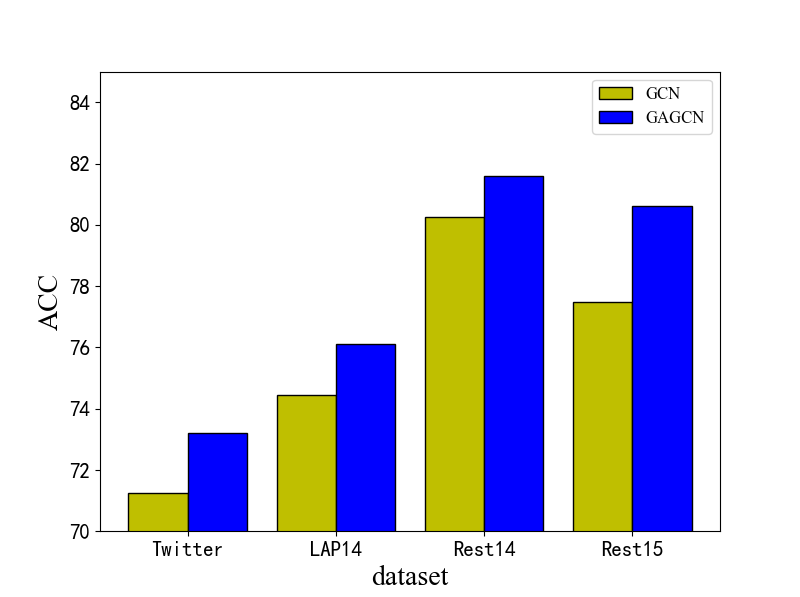
\includegraphics[width=1\textwidth]{pic/gcn-gagcnAcc.png}
%     \caption{分类准确率(ACC)}
%     \label{gcn_gagcn_acc}
%     \end{minipage}
%     \quad
%     \begin{minipage}[t]{0.5\linewidth}
%     \centering
%     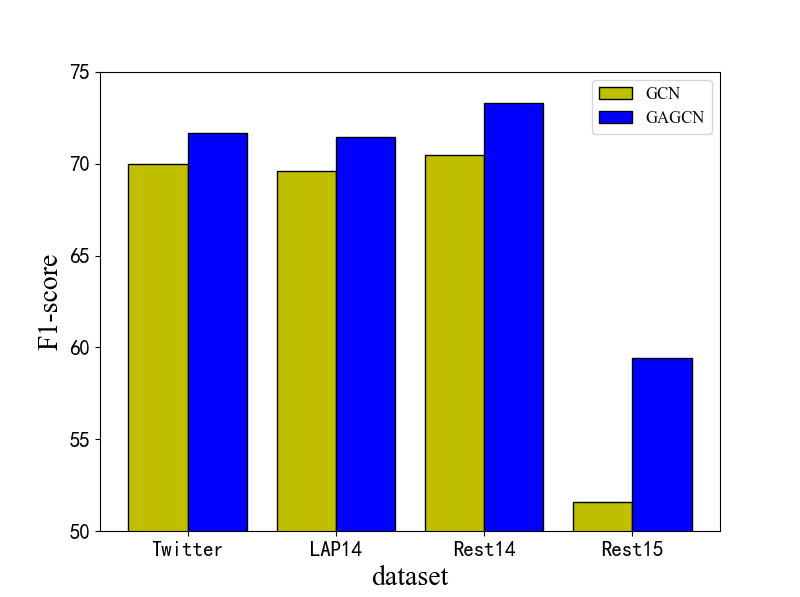
\includegraphics[width=1\textwidth]{pic/gcn-gagcnF1.png}
%     \caption{分类F1分数(F1-score)}
%     \label{gcn_gagcn_f1}
%     \end{minipage}
% \end{figure*}

\begin{figure}[htb]
    \setlength{\belowcaptionskip}{0pt}
    \centering
    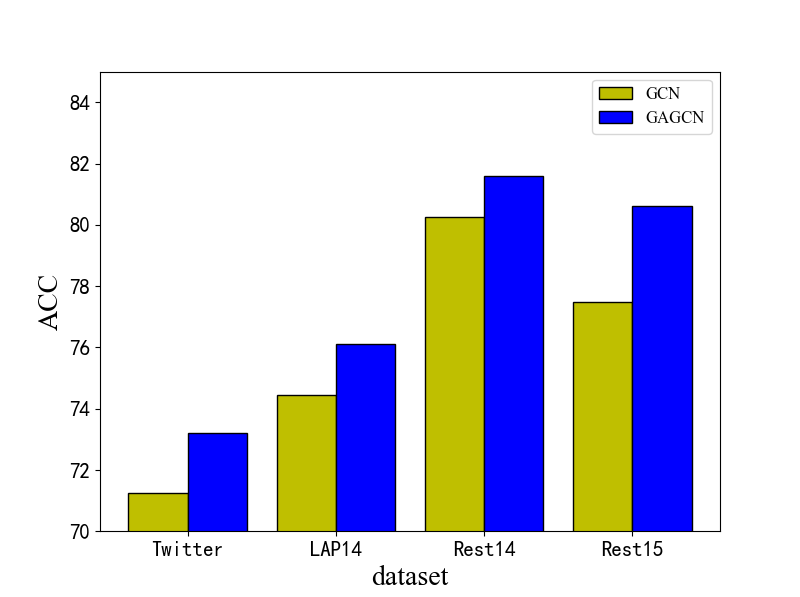
\includegraphics[width=0.8\textwidth]{pic/gcn-gagcnAcc.png}
    \caption{分类准确率(ACC)}
    \label{gcn_gagcn_acc}
\end{figure}

\begin{figure}[htb]
    \setlength{\belowcaptionskip}{0pt}
    \centering
    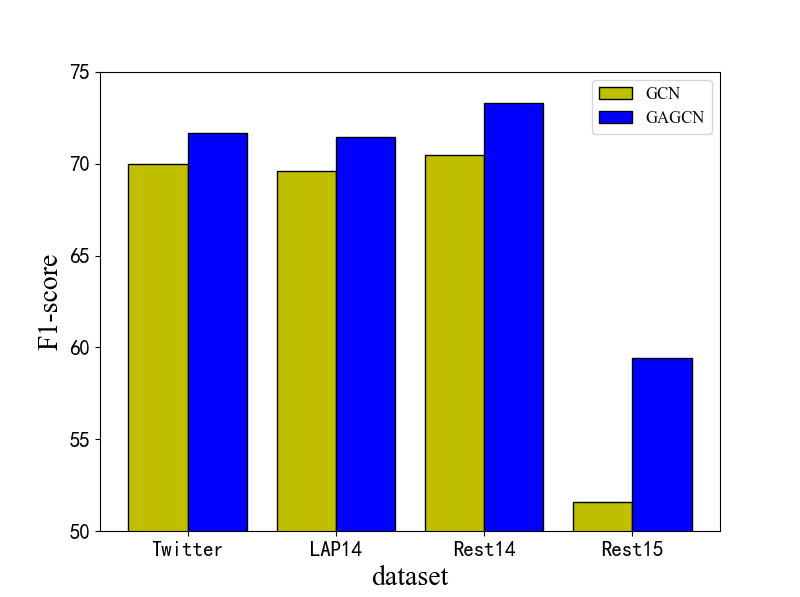
\includegraphics[width=0.8\textwidth]{pic/gcn-gagcnF1.png}
    \caption{分类F1分数(F1-score)}
    \label{gcn_gagcn_f1}
\end{figure}

如图\ref{gcn_gagcn_acc}所示,展示了GAGCN与普通GCN方法的准确率。从图可以看出,在所有的数据集的结果中,GAGCN都明显高于普通的GCN,尤其是在Rest15数据集上高出了3.14个百分点。
说明GAGCN的注意力机制能够辅助模型找到对当前节点贡献度较高的邻居节点,并更多的获取来自这个邻居节点的信息,同时门控机制控制了当前层与上一层节点信息的选取,自适应选择机制可以
帮助模型选择每一层网络中重要的节点信息。F1分数的结果如图\ref{gcn_gagcn_f1},与准确率的结果一致,GAGCN显著高于普通的GCN,
且在Rest15数据集上高出了7.87\%。因此这两个图结果都能证明GAGCN注意力机制和门控机制的有效性。在图节点信息的传播过程中,通过注意力机制挖掘邻居节点之间的关联程度,辅助节点获取到更关键的信息,有助于提升模型性能。

\subsection{数据增扩效果验证}
本节对GAGCN-BERT中提出的数据增扩方法进行了验证。两种形式的参数设置一致,仅有的差异即是在训练过程中是否使用了数据增扩。数据增扩的实现以LAP数据集中的句子“it's color is even cool”为例,这里的
方面词为“color”,在训练的过程中,这句话的方面词有50\%的几率被替换成另一个句子中的方面词,比如“service”,但标签依然维持不变。训练集中的所有句子均有50\%被替换成另一个方面词,而测试集不做替换。
% \begin{figure*}[htb]
%     \begin{minipage}[t]{0.5\linewidth}
%     \centering
%     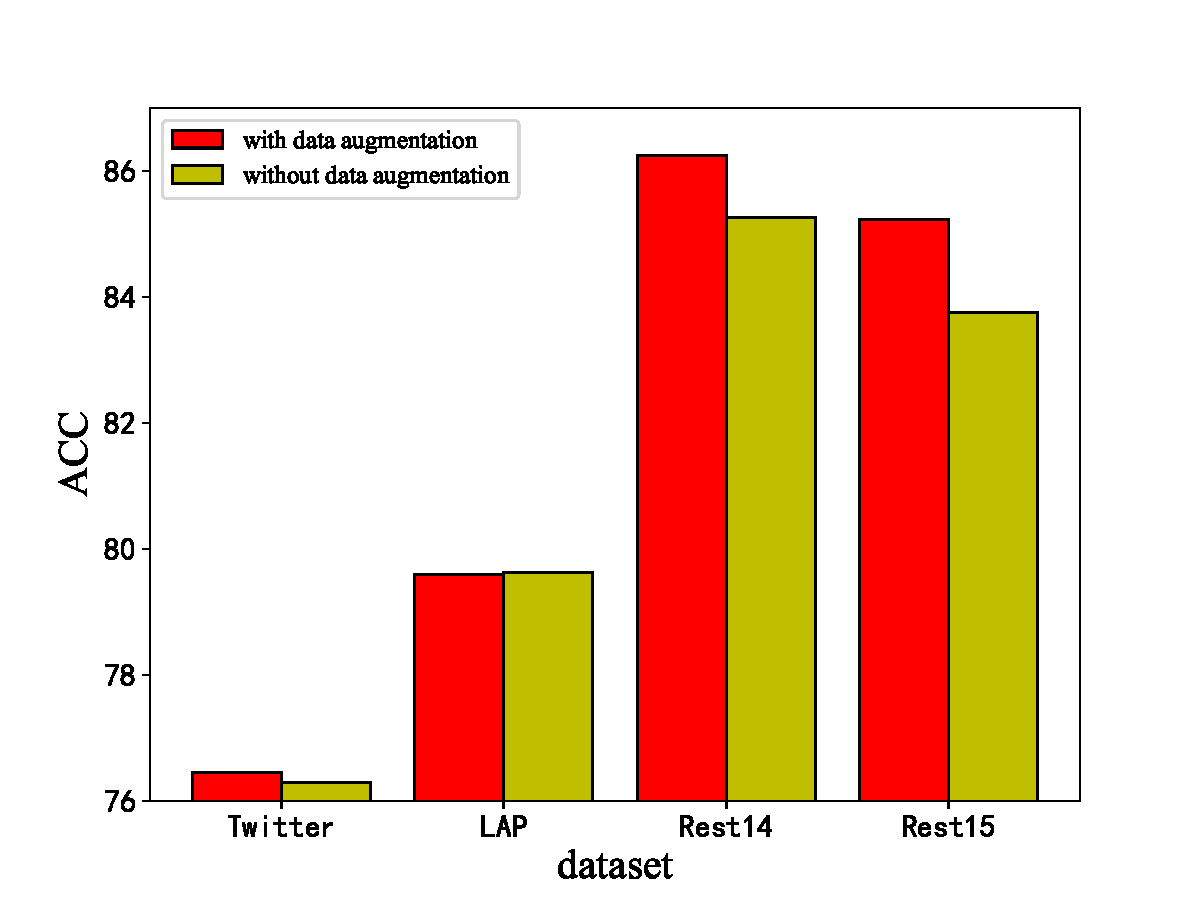
\includegraphics[width=1\textwidth]{pic/DAACC.pdf}
%     \caption{分类准确率(ACC)}
%     \label{DAACC}
%     \end{minipage}
%     \quad
%     \begin{minipage}[t]{0.5\linewidth}
%     \centering
%     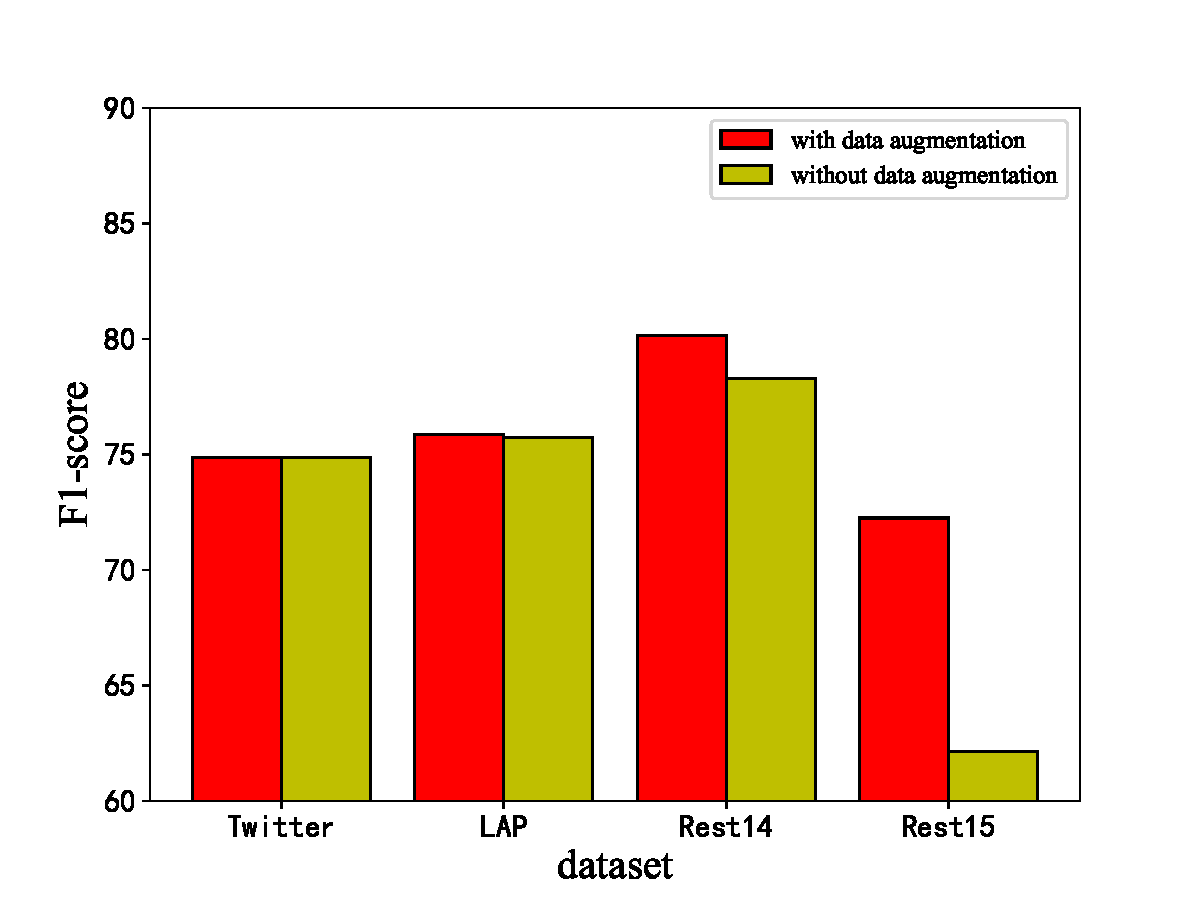
\includegraphics[width=1\textwidth]{pic/DAF1.pdf}
%     \caption{分类F1分数(F1-score)}
%     \label{DAF1}
%     \end{minipage}
% \end{figure*}

\begin{figure}[htb]
    \setlength{\belowcaptionskip}{0pt}
    \centering
    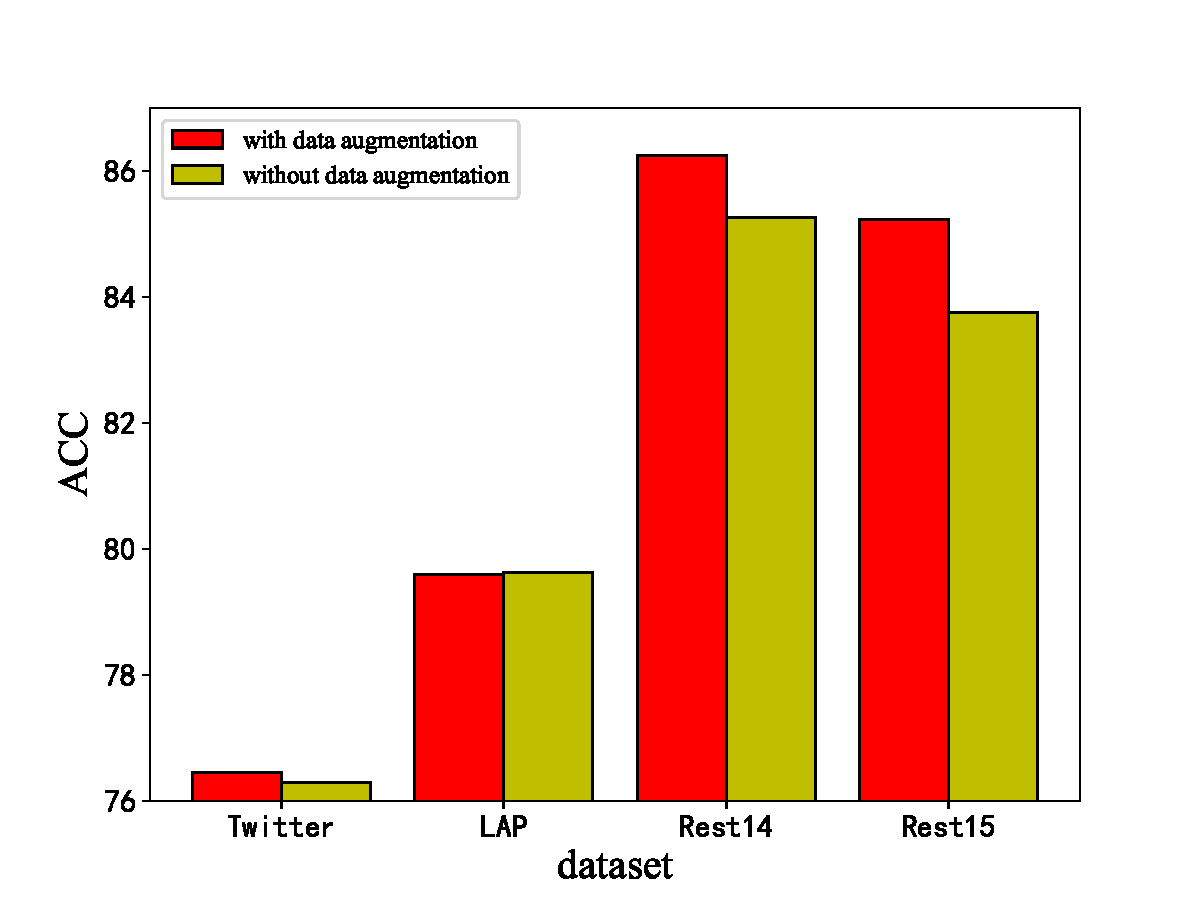
\includegraphics[width=0.6\textwidth]{pic/DAACC.pdf}
    \caption{分类准确率(ACC)}
    \label{DAACC}
\end{figure}

\begin{figure}[htb]
    \setlength{\belowcaptionskip}{0pt}
    \centering
    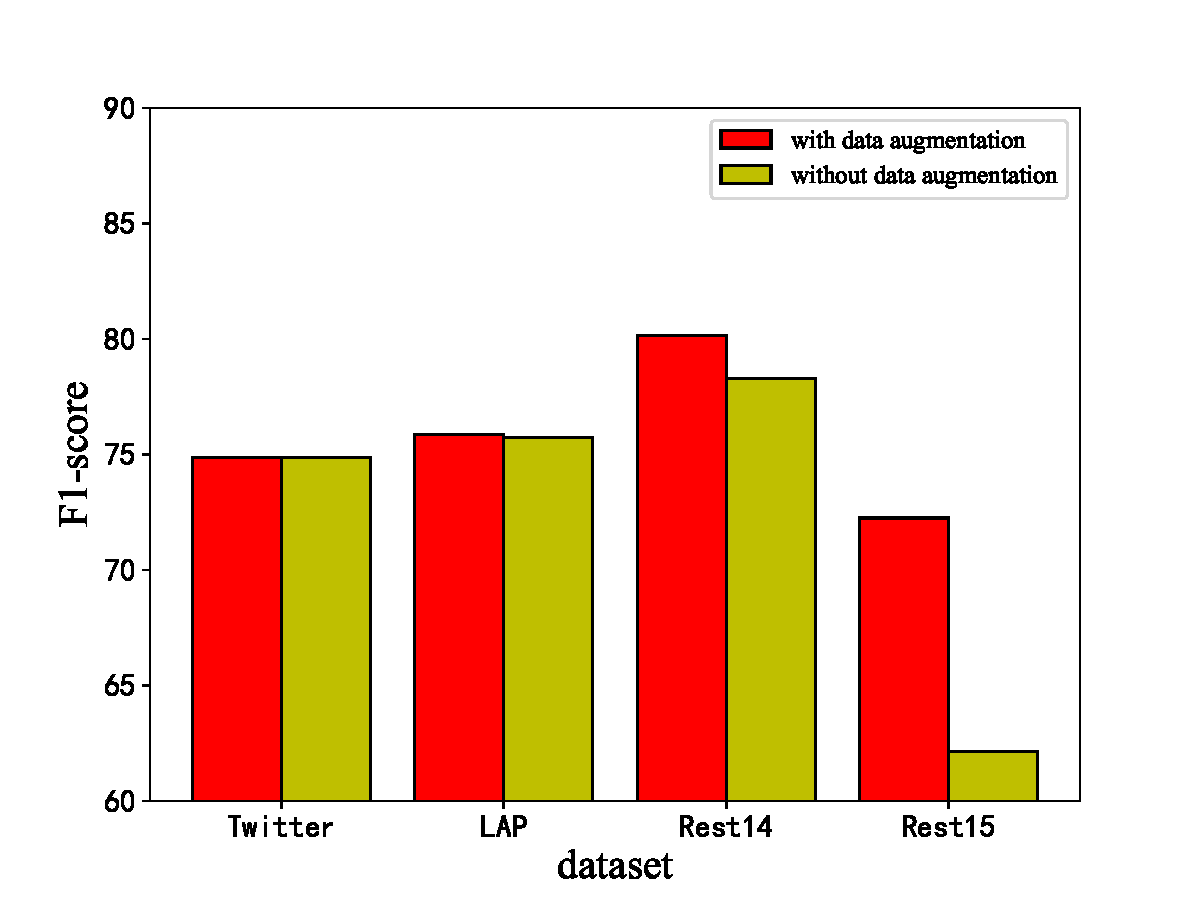
\includegraphics[width=0.6\textwidth]{pic/DAF1.pdf}
    \caption{分类F1分数(F1-score)}
    \label{DAF1}
\end{figure}

如图\ref{DAACC}所示,展示了两种训练方式的分类准确率,从图中可以看出,使用了数据增扩的模型在这四种数据集上基本都高于未使用数据增扩的方法,尤其是在Rest15数据集上,提升了1.47\%。
这可能是由于Rest15数据集相比于其他数据集训练样本更少,模型训练样本不足,容易产生过拟合,故采用数据增扩的方式补充一定量的训练样本,有利于提升模型的泛化能力,提升分类性能。

如图\ref{DAF1}所示,
展示了F1-score的对比差异,与准确率结果类似,使用了数据增扩的方法分类性能优于未使用数据增扩的模型,并且在Rest15数据集上提升了10.1个百分点。差距十分明显。从准确率和F1分数的
结果来看,本章提出的数据增扩方式对模型性能有一定提升,尤其是在仅有少量训练样本的数据集下表现突出。因为这种数据增扩的方式通过替换方面词,让模型学习过程中不过多依赖方面词本身的含义,而去
捕捉语法信息,即方面词所处的上下文位置才是决定情感极性的关键。因此从某种角度上来看这种数据增扩方式一方面增加了训练样本,另一方面引入了人为定义的规则,即让模型不要过多关注于方面词的自身
语义,而去关注于单词间的关系以及语法信息。

\subsection{实验参数比较}
本节比较了不同参数设置条件下模型的分类性能。如图\ref{paraunitacc}所示,比较了设置不同大小神经元个数的GAGCN-BERT模型。由于BERT模型采用的是预训练模型,故未更改BERT中每层网络的神经元个数,而是修改
GAGCN-BERT中GCN每层网络中的神经元个数。

\begin{figure}[htb]
    \setlength{\belowcaptionskip}{0pt}
    \centering
    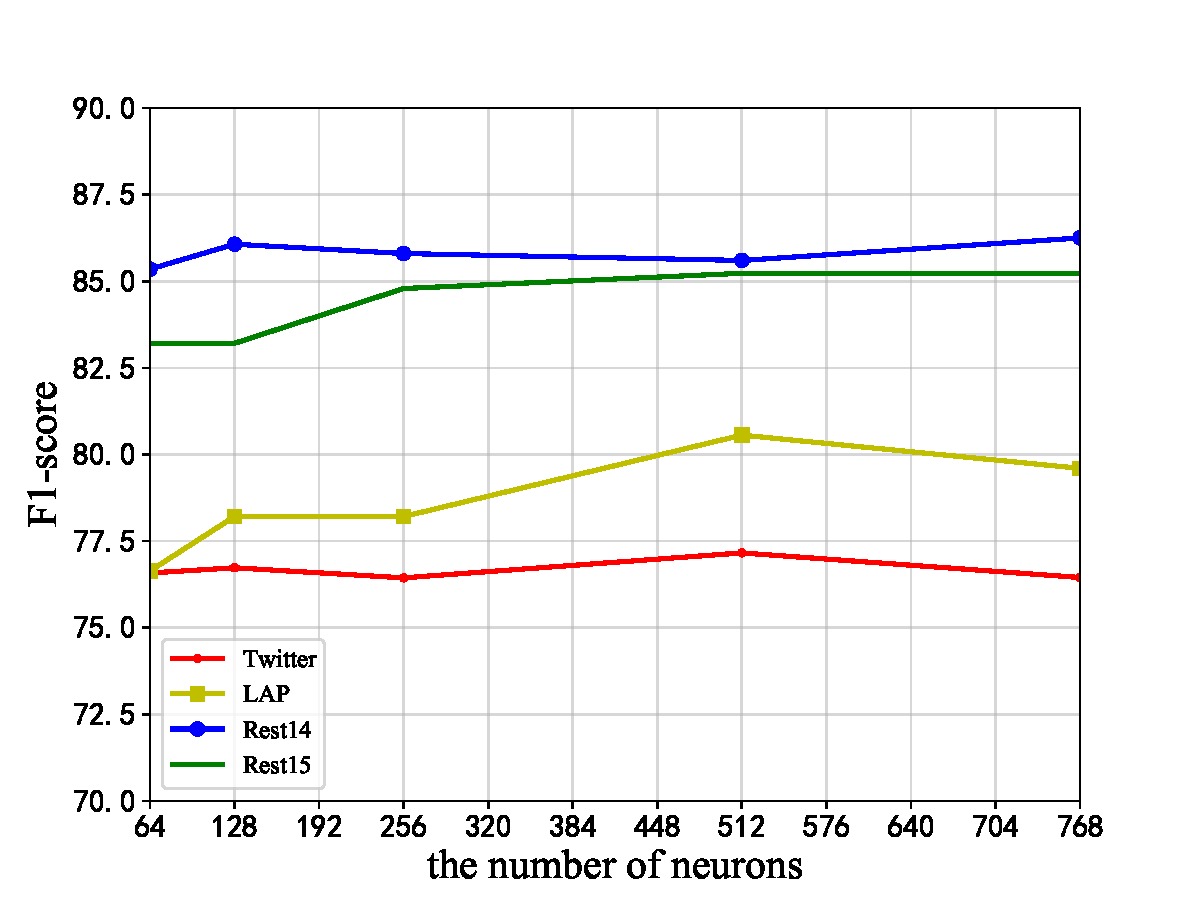
\includegraphics[width=0.6\textwidth]{pic/unitACC.pdf}
    \caption{不同神经元个数比较}
    \label{paraunitacc}
\end{figure}

\begin{figure}[htb]
    \setlength{\belowcaptionskip}{0pt}
    \centering
    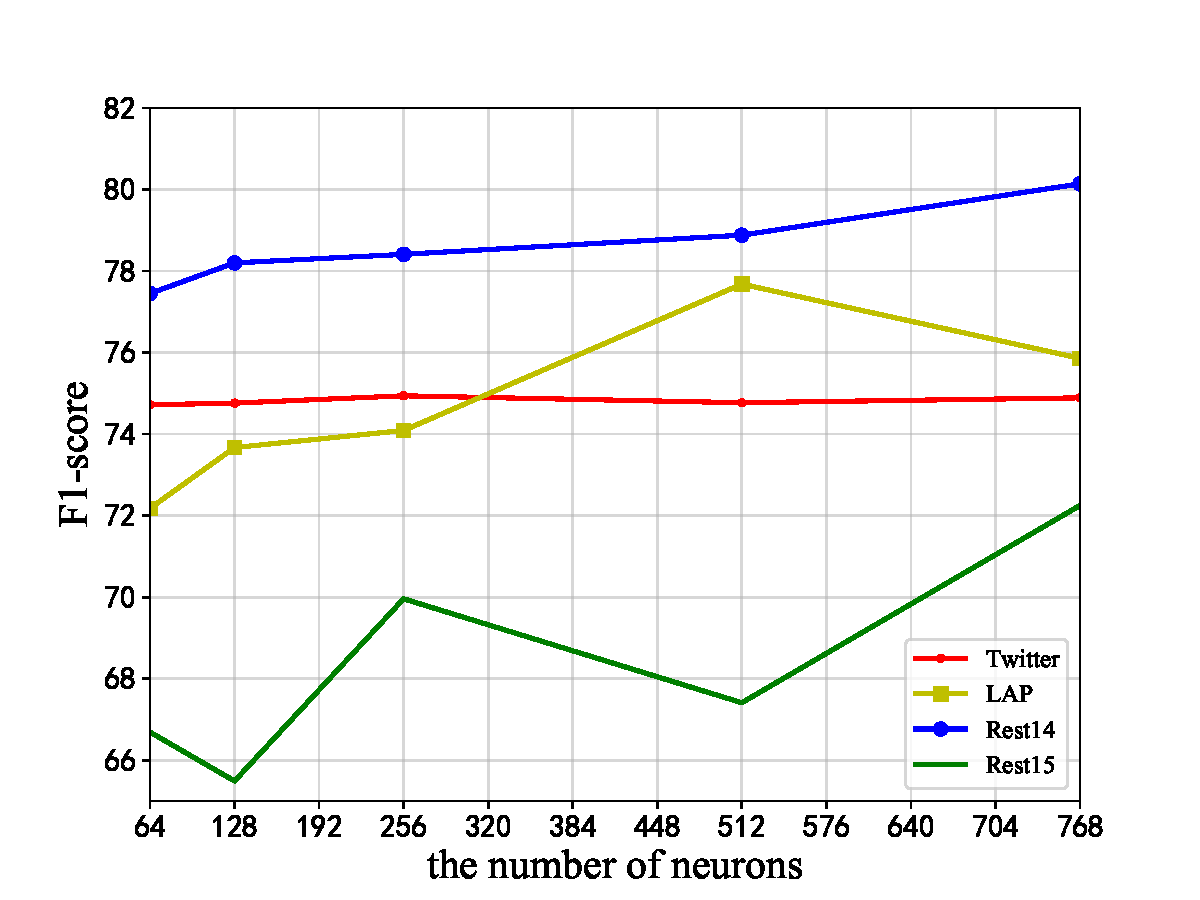
\includegraphics[width=0.6\textwidth]{pic/unitF1.pdf}
    \caption{不同神经元个数比较}
    \label{paraunitf1}
\end{figure}

从图\ref{paraunitacc}中结果来看,该模型的分类准确率对神经元个数不是特别敏感,整体的趋势是随着神经元个数的增加而增加。当神经元个数低于64时分类性能则表现最差,如在LAP数据集上
相比效果最好的模型相差3.92个百分点。这是由于神经元个数非常低时,则所能容纳的信息量将会大幅压缩,从而导致产生的向量信息量较少,无法展现文本数据集
内容信息,故低神经元个数情况下分类性能较差。整体来看,模型在512和768个神经元时表现相对最好。模型F1分数结果如图\ref{paraunitf1}所示。与准确率的趋势一致,整体情况是随着神经元个数的
增加,模型性能也能得到提升。在64个神经元个数时效果最差。

\section{本章小结}
本章介绍了方面级情感分析算法,主要是基于图卷积神经网络以及对第三章算法的延续。建立一个超节点连接方面词中的所有单词,通过GCN网络中节点的信息传递,将方面词中的各个单词进行交互,同时随着
网络层数的加深,也能将超节点的信息传递给文本其他单词,建立超节点与文本上下文中单词之间的联系。注意力机制与门控机制的应用保证节点之间信息的流动具有选择性,即当前节点着重关注于重要的邻居节点,
并从这类节点中获取更多的信息。从结果来看,本章提出的方法在准确率和F1分数上均取得了不错的效果,相比于大多数对比方法均有提升,虽然在部分数据集上不如DGEDT(BiGCN),但是差距细微,且相比之下本章
提出的方法具有更高的计算效率。此外融入了BERT模型进一步提升模型性能,展现了不俗的分类性能。本章还提出了一种数据增扩方式,相比未使用该方法的模型,分类性能有一定的提升。
% \chapter{总结与展望}
\section{本文工作总结}
随着互联网的飞速发展,网络中充斥着大量的文本数据。例如网站论坛上包含了丰富类别的文本数据,如娱乐类信息,政治类新闻,人物描述等。这些文本数据的产生必然伴随着对数据的归类,如何提升分类
效率,减少人工成本,这便是文本数据分类的研究方向。此外在美团、大众点评等网站上具有用户发表的含有感情色彩的评论。从这些海量数据中挖掘出用户的情感,有助于精准地刻画用户,从而辅助平台进行针对性的提供服务。
同时,用户对某一事项的不同方面进行评价,有利于针对这些方面的不足之处进行改进以提升用户感知。方面级情感分类研究便呼之而出。传统的机器学习方法需要大量的手工提取特征的方式,增加了研究者的负担。而一些采用深度学习的方式在文本处理领域略有不足,
例如很多算法忽略了文本的整体信息以及文本在语料库中的统计信息。尤其是在对于方面级目标词与文本内容之间关系的捕捉之上,很多模型都具有改进空间。

基于上述问题,本文提出了一个基于图卷积神经网络的整体文本分类算法和方面级情感分析算法。整体文本分类算法即是对一段文本所属的类别进行归纳,一段文本对应一个标签。方面级
情感分析任务关注于文本中的部分词的情感信息,即一段文本根据目标词汇的不同,可能具有多种情感标签。本文提出的方法采用图模型将单词之间建立联系,并通过这些联系深层次的挖掘
文本语义信息,进而提升模型分类性能。以下是本文的工作内容总结:

(1)对于整体文本分类任务而言,关注的是整体句子的含义。本文提出一种滑动窗口构图的方式,将文本中的不同单词之间建立联系。此外引入了一个超节点,用以连接文本中所有单词,而超节点与
其他节点的边的信息依赖于语料库中文本与单词之间的联系。超节点的创建用以捕获文本整体信息。通过图模型的信息传递机制,将单词节点之间的信息进行交互,并通过一个注意力机制确保节点关注于重要信息。
经过图卷积神经网络的学习后,每个单词节点获得了更加丰富的向量表示,节点之间包含了上下文信息,而超节点通过图模型也获得了整个文本内容的信息。将单词向量构成文本矩阵,再采用CNN网络提取文本中的
关键信息,最后与超节点代表的文本整体信息进行结合,实现文本分类任务。从实验结果来看,本文提出的基于图卷积的整体文本分类算法在准确率和F1分数上均高于对比方法。准确率上在MR数据集上高于第二优的Bi-LSTM模型
1.64个百分点,并远高于MLP7.97\%。对比与同样采用了CNN结构的TextCNN模型来说,准确率和F1分数分别在R52数据集上高出1.43\%和11.18\%,即使是未使用超节点向量的TextGraph-CNN,在R52数据集上准确率高出TextCNN模型
0.8\%,F1分数高出7.27\%,说明本文提出的采用图网络方式学习到的单词向量表示更具有意义。此外,该算法在低比例训练集下展现了不错的分类效果,这种结论与同样采用GCN结构的方法TextGCN类似。超节点向量
和CNN结构提取出的关键信息向量,从两个角度描述了文本信息,因此,从结果来看,两者的结合丰富了文本向量表示,提升了模型分类性能。

(2)对于方面级情感分类任务而言,关注的是当前方面词在文本中的情感色彩。本文依然采用滑动窗口的方式构建文本单词图。不同于整体文本分类算法,超节点不再与所有单词节点建立联系,而仅仅与
方面词建立连接。通过超节点的建立,将方面词中的各个单词融合起来,通过图模型将方面词整体信息传递给方面词中的每个单词,这样促使方面词中各个单词实现紧密联系。此外,随着网络中节点的向更远处
节点的信息传递,有助于将超节点信息传递给上下文中的其他单词,实现方面词与上下文之间的联系。本文还在图卷积神经网络中使用了注意力机制以及门控机制,辅助模型控制信息流动。对于重要的邻居节点
则从中获取更多的信息,对于不重要的节点则选择从中获得少量的信息。从实验结果来看,本文提出的算法在准确率和F1分数上高于绝大多数对比方法。如准确率在Twitter数据集上高于SVM接近9\%,比同样
采用了GCN结构的ASGCN-DT和DGEDT(BiGCN)分别高于1.07\%和0.4\%。尤其是对比未使用注意力机制和门控机制的GCN来说,所有数据集上的表现明显更优,例如在Rest15数据集上准确率和F1分数分别高出3.14\%,
7.87\%。证明本文提出的注意力机制和门控机制的有效性。另外,本文还结合了BERT预训练模型进一步提升模型性能。相比于同样采用了BERT模型的TG-BERT明显更好,如在Rest14数据集上准确率高出1.46\%。
和目前最优的模型之一DGEDT-BERT相比,各有优势。在Twitter数据集上本文的方法略低,但是同样在Rest15数据集上高出1.23\%。同时本文提出的方法相比DGEDT-BERT少了一个计算量较大的transformer结构,在
低计算资源情况下更具优势。最后,本文还提出了一个数据增扩的方式,实验结果表明,能够提升模型分类性能,如在Rest14数据集上提升了1.56\%。

\section{未来工作展望}
文本分类任务是自然语言处理中的关键任务之一。本文提出了基于图模型的文本分类算法,根据具体任务的不同,超节点构建方式具有差异。虽然在实验数据集上展示不错的效果,但仍有许多值得研究和深入的地方:

(1)文本构图方式仅仅采用滑动窗口是不足的,相邻的两个单词之间不一定具有高相关的联系。需要引入其他的构图方式,确保单词之间的边是有意义的。例如语法依赖解析树的方式构建图是一种方式。但是并不是
适用于所有模型,如语法解析树构图方式在本文提出的方法上效果并不好。采用何种构图方式是提升模型性能的关键之一。

(2)文本图生成后,用何种有效的图模型去学习节点之间的信息也值得研究。本文中采用带有注意力机制的图卷积神经网络学习节点信息,进而学到单词丰富的向量表示。但应用于学习图表示的方法不仅限于图卷积神经网络,
现如今已有大量关于图模型的相关研究,提出了多种多样的模型用以处理图结构。不同的模型致力于解决不同的问题,吸纳这些模型的优点可以找出适用于文本图的优秀的图模型。

(3)当引入BERT预训练模型后,算法性能能到很大提升。这是由于训练样本较少,模型难以完全拟合所有情况,因而一个经过大量语料库的预训练的模型有助于提升下游任务的性能。针对某一任务的
训练样本是有限的,因此,一个通用的预训练模型是值得研究的。



%\chapter{template}
This is the template of the chapter in split file.

\section{s1}
This is a section.

\subsection{sub1}
This is a subsection.

% misc

% \thesisacknowledgement
% 光阴似箭,岁月如梭,又到了莺飞草长,万物复苏的季节,三年研究生生涯至此也快要画上一个句号。回首这段时光,增加的不光是我的体重也有知识的厚重,还有研究生期间来自老师
% 和同学朋友之间的情谊。

% 首先最要感谢的是罗老师这段时间的帮助,无论是学习上还是生活上。刚入学校,我还是一个刚刚转业对计算机知识不太了解的学生。罗老师不断地鼓励我,也为了让我快速
% 进入计算机领域,精心为我挑选了许多入门的论文,辅助我学习。当自己对相关概念有一定基础后,引导怎么去我去思考,在学习的过程中还常与我进行相关讨论,指导我研究的方向。
% 回首这几年在教研室的日子过得非常愉快,离不开罗老师的和蔼的性格,真的很好进行交流,有什么问题都可以进行讨论,为人正派,深得我们几个学生私下偷偷拍马屁。同时还给予
% 我们在学习上非常大的自由度。可以凭借自己的兴趣爱好选择学习的方向,并不会给我们过多的限制,反而还会给出相关的指导意见。

% 其次还要感谢教研室的同届同学李光原、彭愈翔。感谢这几年在学习上的互相帮助,通过与他们的交流以及遇到问题时的相互讨论,让我提升很多;感谢唐子超、董又铭等学弟以及隔壁教研室的学霸李家兴在科研上和生活上的帮助,教研室
% 的友好氛围离不开这些同学;感谢室友们在生活中给我带来的无尽的关心和快乐。感谢这些所有人给我这三年的研究生生涯留下了美好的记忆。

% 最后我要感谢我的父母支持我进行转业,对我生活上的关心与帮助,才有了今天的我;感谢科研过程中给予我帮助的朋友老师们和能容纳我的电子科大,以及辛勤工作的审稿老师们。


\thesisappendix

\chapter{中心极限定理的证明}

\section{高斯分布和伯努利实验}

% Uncomment to list all the entries of the database.
% \nocite{*}

\thesisbibliography{reference}

%
% Uncomment the following code to load bibliography database with native
% \bibliography command.
%
% \nocite{*}
% \bibliographystyle{thesis-uestc}
% \bibliography{reference}
%

\thesisaccomplish{publications}

\thesistranslationoriginal
\section{The OFDM Model of Multiple Carrier Waves}



\thesistranslationchinese
\section{基于多载波索引键控的正交频分多路复用系统模型}



\end{document}
